\documentclass{tstextbook}

\begin{document}
\sloppy %added by me to decrease the spillage of words over the right margin of paragraphs.
\tsbook{Μαγνητικές Μελανές Οπές}
       {Χρίστος Σιακάς}
       {Τμήμα Φυσικής}
       {Διατριβή Master}
       {Νικόλαος Τούμπας}
%       {Cover Designer}
%       {2017}
%       {xxxxx}{xxx--xx--xxxx--xx--x}{0.0}
%       {Publisher}
%       {Βόλος}

%---------------------------------------------------------------------------
% Chapters
%---------------------------------------------------------------------------

%---------------------------------------------------------------------------
\chapter{Εισαγωγή}
%\epigraph{}
%Η διατριβή αναφέρεται στην γενίκευση των Schwarzschild μελανών οπών με την ένταξη μαγνητικού μονοπολικού φορτίου. 
\par Η σύζευξη βαρύτητας και ηλεκτρομαγνητισμού
%, εδραιώνεται με τη γενίκευση της γεωμετρίας Schwarzschild. Η %λύση, για σφαιρικώς συμμετρικά σώματα, οδηγεί στη μετρική της  Η %γεωμετρία 
προβλέπει την ύπαρξη φορτισμένων μελανών οπών που περιγράφονται από τη γεωμετρίας Reissner–Nordström.  
%ανωμαλίες με 
Οι φορτισμένες μελανές οπές έχουν κοινά χαραχτηριστικά με τις αφόρτιστες μελανές οπές Schwarzschild 
%μελανών οπών, 
όπως, ορίζοντα, μη μηδενική θερμοκρασία και εντροπία, και εξαϋλώνονται μέσω εκπομπής ακτινοβολίας. 
%η μελανή οπή. 
Σημαντική διαφορά με τις αφόρτιστες μαύρες τρύπες 
%οπές χωρίς φορτίο 
είναι το γεγονός ότι η εξαΰλωση παύει να υφίσταται 
%της εξάτμισης τους, 
όταν η μάζα και το φορτίο ικανοποιούν την ισότητα $GM\superscr{2}=\frac{\pi Q\superscr{2}}{e\superscr{2}}$. Σε αυτή την οριακή περίπτωση, η θερμοκρασία Hawking μηδενίζεται. \\

\par Η διατριβή επικεντρώνεται στη μελέτη μαγνητικά φορτισμένων μαύρων οπών \cite{Maldacena_2021}, λόγω της ευστάθειας τους σε σχέση με τις ηλεκτρικά φορτισμένες. Η μεγάλη μάζα των μαγνητικών μονοπόλων, καταστέλλει τη δημιουργία ζευγών σωματιδίων με θετικό και αρνητικό μαγνητικό φορτίο εντός σχετικά ισχυρών μαγνητικών πεδίων. Σε αντίθεση, η ευστάθεια των ηλεκτρικά φορτισμένων σωμάτων περιορίζεται από το κατώφλι $E\sim 2m\subscr{e}\superscr{2}$ ($\sim 10\superscr{18}V/m$), που προβλέπεται από τη δίδυμο γένεση Schwinger. Κοντά στον ορίζοντα μιας φορτισμένης μελανής οπής ($r\sim MG$), η τιμή του πεδίου είναι $\frac{Q}{M\superscr{2}G\superscr{2}}$. Ηλεκτρικά φορτισμένες οπές με φορτίο και μάζα που ικανοποιούν την ανισότητα $Q\,{\scriptscriptstyle\gtrsim}\,m\subscr{e}\superscr{2}M\superscr{2}G\superscr{2}$
αποφορτίζονται από τα σωματίδια με αντίθετο ηλεκτρικό φορτίο, που δημιουργούνται κατά τη δίδυμο γένεση. Η αποφόρτιση επιτυγχάνεται σε σχετικά σύντομο χρονικό διάστημα, καθιστώντας τις μη ευσταθείς.\\

\par Η ευστάθεια των μαγνητικών πεδίων όμως, δεν παραμένει χωρίς κατώφλι. Για συγκεκριμένες τιμές του μαγνητικού φορτίου και της μάζας δημιουργούν στην εξωτερική περιοχή του ορίζοντα μαγνητικό πεδίο με ένταση ίση με τη μάζα στο τετράγωνο των μποζονίων $W$ της ασθενούς αλληλεπίδρασης. Στην παρουσία τέτοιων μαγνητικών πεδίων λαμβάνουν χώρα διάφορα κβαντικά φαινομένα που οδηγούν σε μια νέα ευσταθή κατάσταση με μη μηδενικό μαγνητικό πεδίο. Τα φαινόμενα εκδηλώνονται σε ακτίνα της τάξης $r\,{\scriptstyle\sim}\,m\subscr{w}\superscr{-1}$ και ενισχύονται εντός της "ηλεκτρασθενούς κορώνας", $m\subscr{h}\superscr{-1}\,{\scriptscriptstyle<}\,r\,{\scriptscriptstyle<}\,m\subscr{w}\superscr{-1}$. Σε ακτίνα $r\,{\scriptstyle\sim}\,m\subscr{h}\superscr{-1}\,{\scriptscriptstyle<}\,m\subscr{w}\superscr{-1}\,$, όπου $h$ to σωματίδιο Higgs, η μη αβελιανή $SU(2)$ συνιστώσα του μαγνητικού πεδίου θωρακίζεται πλήρως, και μένει μόνο η συνιστώσα του αβελιανού $U(1)\subscr{Y}$ υπερφορτίου. 
%πεδίο φτάνει στην ευσταθή κατάσταση. Για μικρότερες ακτίνες το %πεδίο δεν είναι πλέον ο γραμμικός συνδυασμός των συνιστωσών %SU(2) και , αλλά γίνεται ένα εξολοκλήρου υπερμαγνητικό αβελιανό %πεδίο U(1)$\subscr{Y}$. 
Αυτό οφείλεται στη συμπύκνωση ηλεκτρικά φορτισμένων μποζονίων $W$. 
%γεννιούνται κατά τις κβαντικές διακυμάνσεις του κενού, και %αλληλεπιδρούν με το συμβατικό μαγνητικό πεδίο U(1)$\subscr{EM}$. %Η αλληλεπίδραση, οδηγεί σε αστάθειες των μποζονικών πεδίων και %προκαλεί τη δημιουργία συμπυκνώματος W. 
Οι Ambjorn και Olesen βρίσκουν (προσεγγιστικές) λύσεις που περιγράφουν το συμπύκνωμα των μποζονίων $W$, ως ένα περιοδικό πλέγμα κβαντικών δινών στο κάθετο στο μαγνητικό πεδίο επίπεδο \cite{AMBJORN1990193}. 
%διευθύνσεις ως προς το μαγνητικό πεδίο. 
Ένα τέτοιο συμπύκνωμα δημιουργείται στην εξωτερική περιοχή του ορίζοντα μιας σφαιρικά συμμετρικής μαγνητικής μελανής οπής. 
Το συμπύκνωμα αυτό ελαττώνει την ένταση της $SU(2)$ συνιστώσασ του μαγνητικού πεδίου μέχρι την πλήρη θωράκιση του.\\
%μέχρι η ένταση του να φτάσει σε τάξη μεγέθους %${\scriptstyle\sim\,\,m\superscr{2}\subscr{h}/e}$, όπου και %θωρακίζεται εντελώς. 

Το υπερμαγνητικό πεδίο που παραμένει, συζεύγνυται με το υπερφορτίο του Higgs και συνεισφέρει θετικά στην ενεργό μάζα του βαθμωτού πεδίου. Η θετική αυτή συνεισφορά 
%ορίζεται από τα επίπεδα Landau, είναι ανάλογη της έντασης του %υπερπεδίου και 
αναιρεί τη συνεισφορά του αρνητικού όρου μάζας στο δυναμικό του πεδίου Higgs. Η αναίρεση αυτή, καθιστά τη μηδενική τιμή του Higgs ως το μόνο ευσταθές ακρότατο του νέου ενεργού δυναμικού. Στην κατάσταση αυτή, το Higgs έχει μηδενική αναμενόμενη τιμή, η οποία είναι συμμετρική ως προς τους ηλεκτρασθενείς μετασχηματισμούς βαθμίδας $SU(2)\times U(1)\subscr{Y}$, και έτσι παύει η ρήξη της ηλεκτρασθενούς συμμετρίας.\\

\par Η επαναφορά της συμμετρίας εντός της ηλεκτρασθενούς κορώνας επιφέρει την καταστολή του μηχανισμού Higgs. Τα φερμιονικά πεδία καθιστώνται άμαζα και συνεισφέρουν στην ακτινοβολία Hawking. Οι λύσεις της βαρυτικής εξίσωσης Dirac εκδηλώνουν 
%τα απορρέοντα από την οπή, με συνολικό 
εκφυλισμό που είναι ανάλογος του μαγνητικού φορτίου $Q$ της μελανής οπής. Ο εκφυλισμός υπολογίζεται με βάση την ανάλυση του Haldane για το ανάλογο πρόβλημα Landau μη σχετικιστικών σωματιδίων σε σφαιρικά συμμετρικό μονοπολικό μαγνητικό πεδίο. Η ισχύς της ακτινοβολίας Hawking είναι ανάλογη του μαγνητικού φορτίου Q${\scriptstyle>>}$1. Επομένως αποτελεί ένα δραματικά αυξημένο ρυθμό εξάτμισης. 


%---------------------------------------------------------------------------
\chapter{Μαγνητικό Μονόπολο}
\section{Εισαγωγή μαγνητικού μονοπόλου}
\subsection{Ηλεκτρομαγνητισμός Maxwell}
Η κλασική θεωρία Maxwell του ηλεκτρομαγνητισμού περιγράφεται από τις 8 εξισώσεις
\begin{equation}\begin{array}{ll}
        \Vec{\nabla} \cdot \Vec{E} = 4\pi \rho, & \Vec{\nabla} \cdot \Vec{B} = 0 \\
        \Vec{\nabla} \times \Vec{E} = - \frac{\partial \Vec{B}}{\partial t}, & \Vec{\nabla} \times \Vec{B} = 4\pi \Vec{J} + \frac{\partial \Vec{E}}{\partial t}
    \end{array}
\end{equation}

\noindent Σύμφωνα με το νόμο του Gauss περί μαγνητικής ροής, $\Vec{\nabla} \cdot \vec{B} = 0$, μπορούμε να ορίσουμε ένα διανυσματικό πεδίο $\vec{A}$, το οποίο ικανοποιεί 
\begin{equation}\label{curl}
    \vec{B} = \vec{\nabla} \times \vec{A}
\end{equation}

\noindent Το διανυσματικό δυναμικό δεν περιορίζεται απλά σε ένα μαθηματικό "κόλπο", αλλά μαζί με το βαθμωτό ηλεκτρικό δυναμικό συνδυάζονται σε ένα τετραδιάνυσμα, $A_{\mu}$, το οποίο οδηγεί άμεσα στον προσδιορισμό βαθμωτών ποσοτήτων, αναλλοίωτων ως προς μετασχηματισμούς Lorentz. 
Τέτοιες ποσότητες μπορούν με τη σειρά τους να ενταχθούν στη δράση από την οποία εξάγονται οι εξισώσεις κίνησης. \\


\subsection{Ηλεκτρομαγνητισμός στην παρουσία μαγνητικού μονοπόλου}
\noindent Η ύπαρξη μαγνητικών μονοπόλων είναι θεωρητικά αποδεχτή υπό την προϋπόθεση ότι το μαγνητικό φορτίο είναι κβαντωμένο βάση της συνθήκης Dirac, της οποίας η απόδειξη παρουσιάζεται στην επόμενη ενότητα. Το πεδίο ενός τέτοιου φορτίου περιμένουμε να συμπεριφέρεται σε συμφωνία με το πεδίο ενός ηλεκτρικού φορτίου, να φθίνει δηλαδή με το τετράγωνο της απόστασης από την πηγή και να είναι ανάλογο του μαγνητικού φορτίου, το οποίο συμβολίζουμε ως $q_m$. 
\begin{equation}\label{centralB}
    \vec{B} = \frac{q_m \vec{r}}{r^3}
\end{equation}

\noindent Η πυκνότητα του μαγνητικού φορτίου και το αντίστοιχο ρεύμα πρέπει να εισαχθούν στις εξισώσεις του Maxwell. Η κατάλληλη μετατροπή των εξισώσεων οδηγεί στο ακόλουθο συμμετρικό   αποτέλεσμα:

\begin{equation}\label{monem}
    \begin{array}{ll}
        \vec{\nabla} \cdot \Vec{E} = 4\pi \rho_e, & \vec{\nabla} \cdot \Vec{B} = 4\pi \rho_m \\
        \vec{\nabla} \times \vec{E} = - 4\pi \Vec{J}_m - \frac{\partial \Vec{B}}{\partial t}, & \vec{\nabla} \times \vec{B} = 4\pi \Vec{J}_e + \frac{\partial \Vec{E}}{\partial t}
    \end{array}
\end{equation}

\noindent Η μορφή αυτή των εξισώσεων \eqref{monem} απαιτεί περαιτέρω διερεύνηση, όπως φαίνεται από την άμεση σύγκρουση του νόμου $\vec{\nabla}\cdot\vec{B = 4\pi\rho_m}$ με την ύπαρξη ενός διανυσματικού δυναμικού, $\vec{A}$, που να ικανοποιεί την εξίσωση \eqref{curl}. Η σύγκρουση οφείλεται στο γενικό μηδενισμό της απόκλισης του στροβιλισμού ενός καλά ορισμένου διανύσματος
\begin{equation*}
    \vec{\nabla}\cdot\left(\vec{\nabla}\times\vec{A}\right) = 0
\end{equation*}
'Οπως θα δούμε στην επόμενη ενότητα, μπορούμε να ορίσουμε δυναμικό - το οποίο όμως δεν είναι πεπερασμένο παντού στο χώρο - που να αποτρέπει την πιο πάνω αντίφαση, και στη συνέχεια θα αποδείξουμε ότι, στο πλαίσιο της θεωρίας μετασχηματισμών βαθμίδας, ο απειρισμός του $\vec{A}$ είναι ασήμαντος. Θα ακολουθήσουμε την ανάλυση του \cite{Jackson:100964}.
%\newpage
\begin{figure}[t]
    \centering
    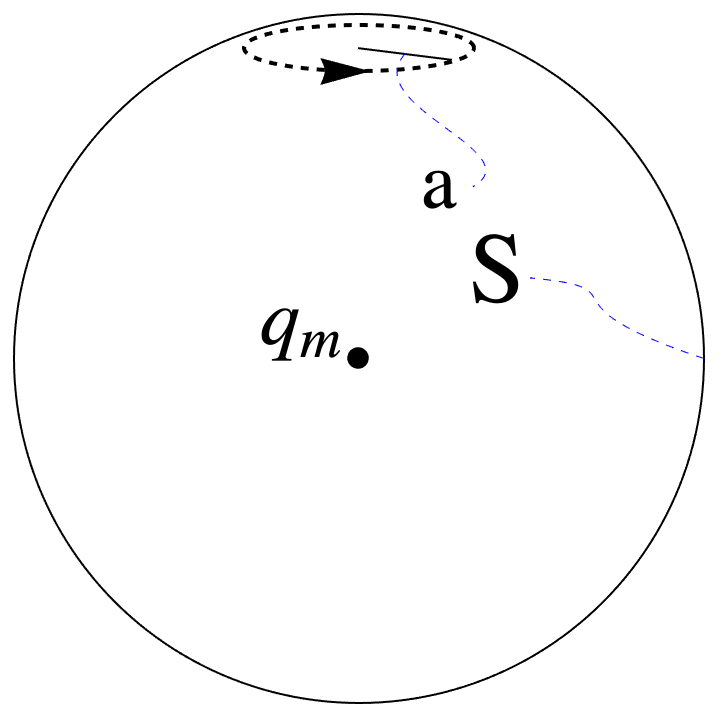
\includegraphics[width=3.5cm, height=3.5cm]{Magnetic Monopole Sketch.png}
    \caption{\textit{Ανοιχτή επιφάνεια $S$. Ο διακεκομμένος κύκλος ακτίνας $a$ είναι σύνορο της $S$}}
    \label{fig:opensurf}
\end{figure}
\section{Συνθήκη Κβάντωσης Dirac}
\noindent Οι συμμετρίες των εξισώσεων \eqref{monem} ωθούν προς την αναζήτηση κάποιου δυναμικού $\Vec{A}$, ικανού να μας δώσει  μέσω της \eqref{curl} ένα κεντρικό μαγνητικό πεδίο. Το μαγνητικό πεδίο $\vec{B}$ πρέπει - όντας ένα μετρήσιμο φυσικό μέγεθος - να είναι καλά ορισμένο παντού στο χώρο, εκτός από τη θέση του σημειακού μονοπόλου ($r = 0$). Η μαγνητική ροή τότε, δίνεται από τον ολοκληρωτικό νόμο Gauss 
\begin{equation}\label{intGauss}
    \int\limits_V \vec{\nabla} \cdot \Vec{B}\, dV = \oint\limits_{\partial V = S} \Vec{B} \cdot d\Vec{s} = 4\pi q_m
\end{equation}

\noindent όπου το επιφανειακό ολοκλήρωμα πραγματοποιείται ως προς την κλειστή επιφάνεια που περιβάλει το μαγνητικό μονόπολο. %- και πρέπει να ισούται με την συνολική μαγνητική ροή διαμέσου %της επιφάνειας. 
%Η 'αδυναμία' του δυναμικού $\vec{A}$ γίνεται εμφανής 
Εάν επιχειρήσουμε να αντικαταστήσουμε την \eqref{curl} στην \eqref{intGauss}, καταλήγοθμε σε μηδενική μαγνητική ροή διαμέσου της επιφάνειας
\begin{equation*}
    \int\limits_V \vec{\nabla} \cdot \left( \vec{\nabla} \times \vec{A} \right) \, dV = 0
\end{equation*}

\subsection{Διανυσματικό δυναμικό με απροσδιοριστίες}
 Για να αποφύγουμε τον μηδενισμό, θα αναθεωρήσουμε το κλειστό επιφανειακό ολοκλήρωμα \eqref{intGauss}. Το ολοκλήρωμα ως προς μια ανοιχτή επιφάνεια $S$ (σχήμα \ref{fig:opensurf}), με βάση το θεώρημα του Stokes, ανάγεται σε επικαμπύλιο και εκτελείται κατά μήκος του κλειστού βρόχου που αποτελεί το σύνορο της ανοιχτής επιφάνειας. Πρέπει να επισημάνουμε ότι αρχικά η διανυσματική συνάρτηση $\vec{A}$ θεωρείται καλά ορισμένη στην $S$:

\begin{equation}\label{lineint}
    \int\limits_{S}  \vec{B} \cdot d\vec{s} = \int\limits_{S}(\vec{\nabla}\times \vec{A} )\cdot d\vec{s} = \oint\limits_{\partial S} \vec{A} \cdot d\vec{\ell}
\end{equation}

Χωρίς βλάβη γενικότητας, επιλέγουμε την $S$ ώστε το σύνορο της να είναι ένας κύκλος με ακτίνα $a$ και άξονα συμμετρίας τον καρτεσιανό άξονα $z$. Το στοιχειώδες μήκος του επικαμπύλιου ολοκληρώματος \eqref{lineint} ισούται με $d\Vec{\ell} = a \,\, d\phi \,\, \hat{\phi}$. Στο όριο όπου η ακτίνα του κύκλου τείνει στο μηδέν, αναμένουμε ότι το επικαμπύλιο ολοκλήρωμα μηδενίζεται, εάν το διανυσματικό δυναμικό είναι παντού καλά ορισμένο, κάτι όμως που οδηγεί σε ασυμφωνία με τη ροή του μονοπόλου:
\begin{equation}\label{limofbound}
    \lim\limits_{a\rightarrow0}\oint\limits_{\partial S} \Vec{A} \cdot \left(  a \,\, d\phi \,\, \hat{\phi} \right) = 0 \quad \ne \oint\limits_{\partial V = S} \Vec{B} \cdot d\Vec{s} 
\end{equation}

\begin{figure}[t]
            \centering
            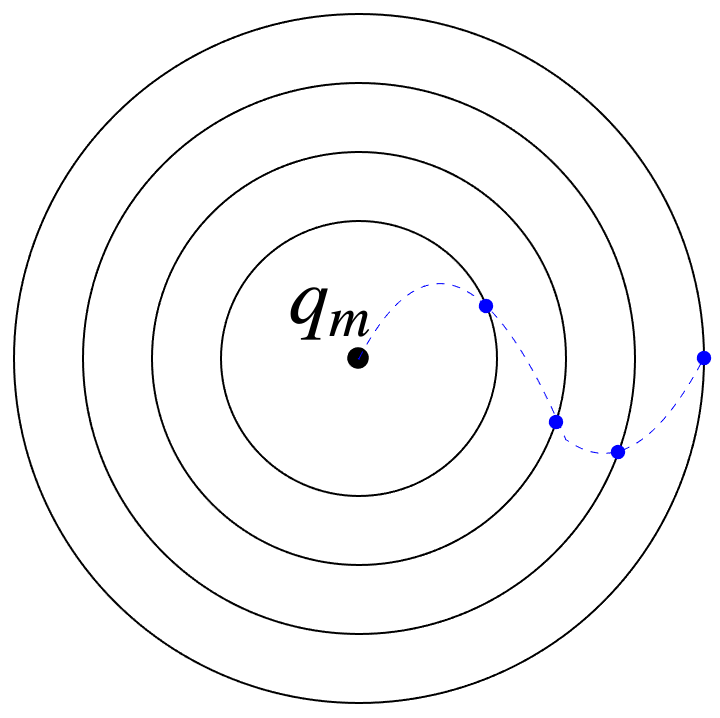
\includegraphics[width=4cm, height=4cm]{Magnetic Monopole String Sketch.png}
            \caption{\textit{Διαδοχικές ομόκεντρες επιφάνειες η κάθε μία από τις οποίες έχει ένα μοναδικό σημείο στο οποίο η συνάρτηση $\vec{A}$ δεν ορίζεται.}}
    \label{fig:diracstr}
\end{figure}
\subsection{Χορδή Dirac}
Για να αναιρέσουμε την ασυμφωνία της \eqref{limofbound}, θεωρούμε λοιπόν ότι το διανυσματικό πεδίο $\vec{A}$ είναι καλά ορισμένο παντού στην $S$, εκτός από ένα σημείο. Έτσι, το επικαμπύλιο ολοκλήρωμα \eqref{limofbound} μπορεί να είναι διάφορο από μηδέν, αλλά πεπερασμένο, ακόμα και στο όριο $a \rightarrow 0$:

\begin{equation*}
            \lim\limits_{a\rightarrow0}\oint\limits_{\partial S} \vec{A} \cdot d\vec{\ell} \ne 0
\end{equation*}
%Η αυθερεσία ως προς τις διαστάσεις της σφαιρικής επιφάνειας S - %που επιβάλλεται όπως περιλαμβάνει την κατανομή φορτίου - %αντικατοπτρίζει την ανεξαρτησία, του θεωρήματος Gauss, από την %επιφάνεια. 
Το θεώρημα Gauss ισχύει για κάθε επιφάνεια που περιβάλει το μαγνητικό μονόπολο, ανεξάρτητα από το σχήμα και το μέγεθος της. Στο σχήμα \ref{fig:diracstr} παρουσιάζονται τέτοιες ομόκεντρες σφαίρες των οποίων τα σημεία απροσδιοριστίας του $\vec{A}$ έχουν τεπιλεγεί και τοποθετηθεί με τέτοιο τρόπο, ώστε για αυθαίρετα μεγάλο αριθμό επιφανειών να σχηματίζουν μια συνεχή καμπύλη. Η καμπύλη αυτή αρχίζει από το σημειακό μονόπολο στο κέντρο και εκτείνεται στο άπειρο. Η καμπύλη ονομάζεται χορδή Dirac. 
%θα επιμείνω σε αυτή την ονομασία για το υπόλοιπο του κειμένου. 
Μια φυσική διάταξη η οποία μπορεί να αναπαραστήσει τη χορδή Dirac, \ref{fig:diracstr}, αποτελεί μια γραμμική κατανομή απειροστά μικρών μαγνητικών διπόλων κατά μήκος ημιευθείας. Η διάταξη αυτή παράγει ένα διανυσματικό δυναμικό με τις ιδιότητες του $\vec{A}$. 
%Αν και στην πραγματικότητα μια ημιάπειρη συνοχή από μαγνητικά %δίπολα δεν είναι υλοποιήσιμη 
Όπως θα δούμε, μετασχηματισμοί βαθμίδας προκαλούν παραμορφώσεις της χορδής Dirac στο χώρο και παράγουν διαφορές φάσεως σε ένα κβαντικό σύστημα.

\subsection{Xορδή Dirac από μαγνητικά δίπολα}
Ένα απειροστό μαγνητικό δίπολο το οποίο αποτελείται από δύο αντίθετα σημειακά μονόπολα $q_m$, $-q_m$, με τη μετατόπιση μεταξύ τους να ισούται με $d\vec{\ell}$, έχει μαγνητική διπολική ροπή
\begin{equation}
    d\vec{m} = q\subscr{m} d\vec{\ell}
\end{equation}
Η συνεισφορά στο διανυσματικό δυναμικό $d\vec{A}$ στη θέση $\vec{x}$ ενός τέτοιου μαγνητικού διπόλου $d\vec{m}$ στη θέση $\vec{x}'$ δίνεται από την έκφραση 
\begin{equation}\label{dipolecontr}
    d\vec{A}(x) \, = \, d\vec{m} \times \frac{(\vec{x}-\pvec{x}')}{|\vec{x}-\pvec{x}'|^3} \, = \, - d\vec{m}\times \vec{\nabla}\left( \frac{1}{|\vec{x}-\pvec{x}'|} \right)
\end{equation}
όπου στη δεύτερη εξίσωση έγινε χρήση της \eqref{apx_1}. 
%\newpage
\begin{figure}[t]
    \centering
    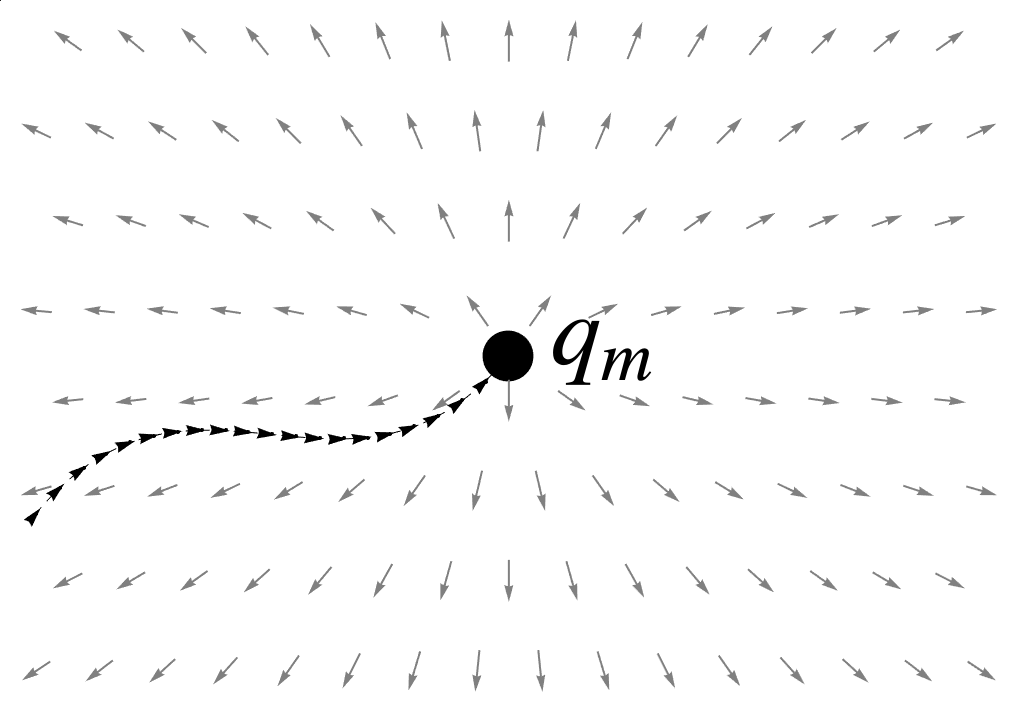
\includegraphics[width=7cm, height=5cm]{monopole field.png}
    \caption{\textit{Μαγνητικά δίπολα (μαύρα βέλη) συνιστούν χορδή Dirac η οποία καταλήγει στο μαγνητικό μονόπολο.}}
    \label{fig:monopfield}
\end{figure}
%Η σύνδεση των πολυάριθμων διπόλων είναι απλά το άθροισμα των %απειροελάχιστα μικρών ροπών που με τη σειρά του γράφεται ως 
Το συνολικό διανυσματικό δυναμικό δίδεται από το επικαμπύλιο ολοκλήρωμα \footnote{$\qquad- d\pvec{\ell}'\times \vec{\nabla}\left(\frac{1}{|\vec{x}-\pvec{x}'|}\right) \, = \, \vec{\nabla}\left(\frac{1}{|\vec{x}-\pvec{x}'|}\right) \times d\pvec{\ell}'\, = \, \vec{\nabla}\times\left(\frac{d\pvec{\ell}'}{|\vec{x}-\pvec{x}'|}\right)$
}
\begin{equation}\label{vectorpot}
    \vec{A}(\vec{x}) \, =  \, -q\subscr{m}\int\limits_L d\pvec{\ell}'\times \vec{\nabla}\left(\frac{1}{|\vec{x}-\pvec{x}'|}\right) \, = \, q\subscr{m}\,\vec{\nabla}\times \int\limits_L \frac{d\pvec{\ell}'}{|\vec{x}-\pvec{x}'|}
\end{equation}
κατά μήκος της χορδής Dirac και ο τελεστής κλίσης δρα στη μεταβλητή $\vec{x}$. Το μαγνητικό πεδίο 
%που αντιστοιχεί στο διανυσματικό δυναμικό της χορδής Dirac, 
%υπολογίζεται ανατρέχοντας πίσω στην εξίσωση 
δίδεται από τη σχέση \eqref{curl}:
%, όπου αντικαθιστούμε την \eqref{vectorpot}. 
\begin{equation}\label{fieldwstr}
\begin{split}
        \Vec{B} &= \vec{\nabla} \times \left( \vec{\nabla} \times \int\limits_L \frac{q\subscr{m}\,d\pvec{\ell}'}{|\vec{x}-\pvec{x}'|}\right)\\
        &= q\subscr{m}\,\vec{\nabla}\int\limits_L \vec{\nabla}\cdot\left(\frac{d\pvec{\ell}'}{|\vec{x}-\pvec{x}'|}\right) - q\subscr{m}\int\limits_L \vec{\nabla}^2\left(\frac{1}{|\vec{x}-\pvec{x}'|}\right)d\pvec{\ell}' \\
        &= \underbrace{q\subscr{m}\frac{\vec{x}-\pvec{x}\subscr{0}}{|\vec{x}-\pvec{x}\subscr{0}|^3}}_{B_{mon}} \, + \, \underbrace{4\pi q\subscr{m} \int\limits_L \delta^3\left(\vec{x}-\pvec{x}'\right)\,d\pvec{\ell}'}_{B_{χορδή}}
\end{split}
\end{equation}
Το άκρο της χορδής βρίσκεται στη θέση $\vec{x}\subscr{0}$. Για την εξαγωγή της δεύτερης ισότητας χρησιμοποιούμε την \eqref{apx_3}. Ο πρώτος όρος του τελικού αποτελέσματος ισούται με το πεδίο του μαγνητικού μονοπόλου. (Οι πράξεις παρουσιάζονται στην \eqref{apx_5}). Ο δεύτερος όρος, βάσει της ταυτότητας \eqref{apx_4}, δείνει το πεδίο της χορδής Dirac, το οποίο δεν προσδιορίζεται. Στο σχήμα \ref{fig:monopfield} αναπαρίσταται γραφικά το συνολικό αποτέλεσμα της \eqref{fieldwstr}. Εχουμε λοιπόν καταλήξει στο ζητούμενο πεδίο του μαγνητικού μονοπόλου, με μια όμως επιπρόσθετη ανεπιθύμητη απροσδιοριστία. Για την εγκυρότητα του πεδίου, επιβάλλεται όπως η απροσδιοριστία αυτή καταστεί μη παρατηρήσιμη. 

%\newpage

\subsection{Μετασχηματισμοί βαθμίδας και χορδή Dirac}
%Σκοπός της παρούσας ενότητας είναι αρχικά η μελέτη της σχέσης %μεταξύ διαμορφώσεων της χορδής Dirac. 
Παρατηρούμε ότι ο πρώτος όρος της \eqref{fieldwstr} είναι ανεξάρτητος του σχήματος της χορδής. Μπορούμε δηλαδή, να παραμορφώσουμε τη χορδή Dirac (αλλάζοντας την καμπύλη $L$), κρατώντας το άκρο της σταθερό, και παίρνουμε το ίδιο πεδίο μαγνητικού μονοπόλου με διαφορετική χορδή.\\

Αντιθέτως, αναμένουμε ότι το διανυσματικό δυναμικό  \eqref{vectorpot} θα μεταβληθεί. Στο πλαίσιο της κβαντικής θεωρίας, η μεταβολή μπορεί να αναπαραχθεί με έναν μετασχηματισμό βαθμίδας \cite{Sakurai:1167961}, ο οποίος μετασχηματίζει τις κυματοσυναρτήσεις
\begin{equation}\label{gtfun}
    \scafun{\Psi}{\vec{x}} \,=\, \scafun[0]{\Psi}{\vec{x}}e^{iq \scafun{\Lambda}{\vec{x}}}
\end{equation}
όπου το $\Lambda$ είναι μια βαθμωτή, μονότιμη και πραγματική συνάρτηση των (x,y,z) και $\Psi_0$ η αρχική κυματοσυνάρτηση. Η κλίση της συνάρτησης $\Lambda$ 
%συσχετίζεται με το αρχικό ($\vecfun[L]{A}{\vec{x}}$) και %μετασχηματισμένο ($\vecfun[L']{A}{\vec{x}}$) 
πρέπει να ισούται με τη μεταβολή του διανυσματικού δυναμικού ως εξής
\begin{equation}\label{gaugetransform}
    \vec{\nabla} \Lambda \,=\, \vecfun[L']{A}{\vec{x}} - \vecfun[L]{A}{\vec{x}}
\end{equation}
Στην περίπτωση της χορδής Dirac όμως, η μεταβολή στο δεξιό μέλος της \eqref{gaugetransform}, αν και μονότιμη συνάρτηση, δεν μπορεί να γραφτεί άμεσα ως η κλίση μιας βαθμωτής συνάρτησης $\Lambda$ εξαιτίας ενός επιπρόσθετου όρου. Στο επόμενο κεφάλαιο θα αποδείξουμε τη συνθήκη κβάντωσης 
%συνθήκη που αποδυκνύει περίτρανα 
του Dirac \cite{Dirac:1931kp}, η οποία καθιστά τις μεταβολές που προκύπτουν, λόγω των παραμορφώσεων της χορδής, μη 
παρατηρήσιμες.\\

Ας θεωρήσουμε λοιπόν δύο χορδές, τις $L$ και $L'$, όπως φαίνεται στο σχήμα \ref{fig:twostrconf}. Επειδή το διανυσματικό δυναμικό ενός μαγνητικού διπόλου
%\footnote{Στο όριο όπου η θέση του διπόλου, $\vec{x}'$ είναι %αρκετά μακριά από τη θέση εξέτασης δυναμικού, $\vec{x}$, έχουμε %\\
%\indent $|d\vec{A}(x)| \, \sim \, %\lim\limits\subscr{|\Vec{x}-\Vec{x}'|\rightarrow %\infty}\frac{1}{|\Vec{x}-\Vec{x}'|^2} \sim 0$ } %\eqref{dipolecontr}, 
φθίνει πολύ γρήγορα (με το τετράγωνο της απόστασης από τη θέση του διπόλου)
μπορούμε, χωρίς βλάβη γενικότητας, να ενώσουμε τις δύο χορδές στο άπειρο. \\

\begin{figure}[t]
    \centering
    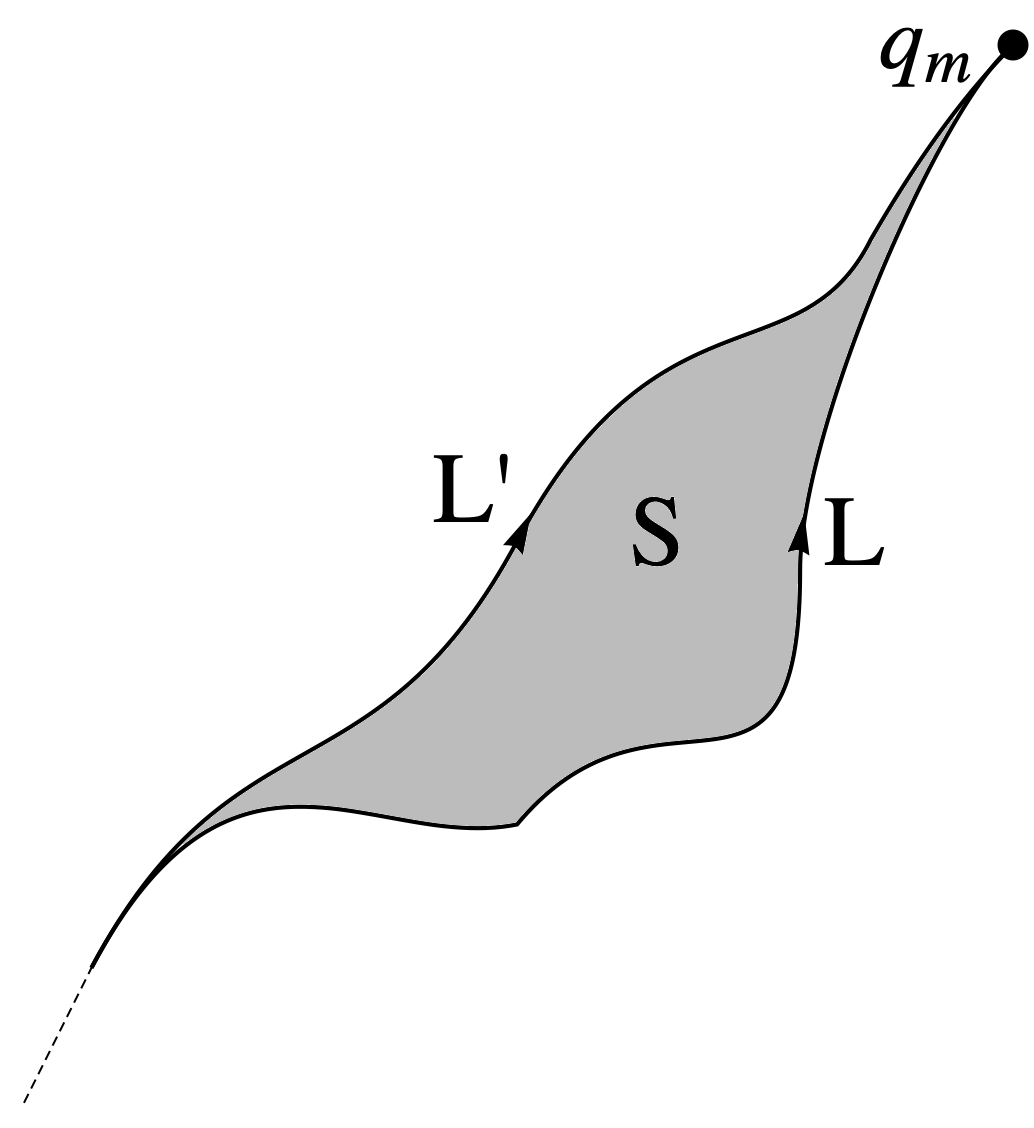
\includegraphics[width=4.5cm, height=4.5cm]{diracstrings}
    \caption{\textit{Δύο ημιάπειρες χορδές Dirac καταλήγουν στο ίδιο σημείο (μαγνητικό μονόπολο). Μακριά από το σημείο όπου απορρέει το μονοπολικό πεδίο, θεωρούμε ότι οι χορδές αλληλοεπικαλύπτονται.}}
    \label{fig:twostrconf}
\end{figure}
%\newpage

Όπως έχουμε ήδη αναφέρει, κάθε χορδή παράγει ένα συγκεκριμένο δυναμικό. Έτσι, για τις δύο χορδές $L$, $L'$ παίρνουμε τα δυναμικά $\vec{A}\subscr{L}$ και $\vec{A}\subscr{L'}$. Η κλειστή διαδρομή $C$, που σχηματίζουν οι δύο χορδές, καθορίζει τη διαφορά των δυναμικών ως εξής
\begin{equation}\label{vecpotdif1}
    \vecfun[L']{A}{\vec{x}} - \vecfun[L]{A}{\vec{x}} \, = \, q\subscr{m}\,\vec{\nabla}\times \left(\int\limits_{L'} \frac{d\pvec{\ell}'}{|\vec{x}-\pvec{x}'|} - \int\limits_L \frac{d\pvec{\ell}'}{|\Vec{x}-\pvec{x}'|} \right) \, = \, q\subscr{m}\,\vec{\nabla}\times \oint\limits_C \frac{d\pvec{\ell}'}{|\Vec{x}-\pvec{x}'|}
\end{equation}

Εφαρμόζουμε τώρα το θεώρημα του Stokes στο κλειστό επικαμπύλιο ολοκλήρωμα της \eqref{vecpotdif1} (παράρτημα \ref{apx22}) και παίρνουμε 
%το επιφανειακό ολοκλήρωμα
\begin{equation}\label{vecpotdif2}
    q\subscr{m}\,\vec{\nabla}\times \oint\limits_C \frac{d\pvec{\ell}'}{|\Vec{x}-\pvec{x}'|}\, =\, q\subscr{m} \, \vec{\nabla}\times\left(\vec{\nabla}\times\int\limits_S \frac{d\pvec{s}'}{|\vec{x}-\pvec{x}'|}\right)
\end{equation}

Με χρήση της ταυτότητας \eqref{apx_3} καταλήγουμε στους ακόλουθους δύο όρους 
\begin{equation}\label{vecpotdif3}
    \vecfun[L']{A}{\vec{x}} - \vecfun[L]{A}{\vec{x}} \,=\, \text{\scalebox{1.5}{$\vec{\nabla}$}} \Bigg(q\subscr{m}\underbrace{\int\limits_S \frac{\pvec{x}'-\vec{x}}{|\vec{x}-\pvec{x}'|^3}\cdot d\pvec{s}'}_{\scafun{\Omega}{\vec{x}}}\Bigg) \,\,\,+\,\,\, 4\pi q\subscr{m} \,\int\limits_S \scafun[][3]{\delta}{\vec{x}-\pvec{x}'} \, d\pvec{s}'
\end{equation}

όπου ο πρώτος όρος είναι η στερεά γωνία που σχηματίζει η επιφάνεια $S$ ως προς το σημείο $\vec{x}$. Ο δεύτερος όρος προκύπτει από την ταυτότητα \eqref{apx_4}. Η διαφορά δυναμικού \eqref{vecpotdif3} εξαρτάται από τη στερεά γωνία της επιφάνειας $S$ μεταξύ των χορδών και ενός απροσδιόριστου όρου - ο οποίος θα αποδειχθεί μη παρατηρήσιμος. \\

\subsection{Συνθήκη κβάντωσης Dirac}

Στο παράδειγμα του παραρτήματος \ref{apx23} γίνεται εφαρμογή των πιο πάνω αποτελεσμάτων και αποδεικνύεται ότι η \eqref{vecpotdif3} μπορεί να ταυτιστεί με ένα μετασχηματισμό βαθμίδας. Συνοπτικά γράφουμε

\begin{equation*}
    L\rightarrow L' \Rightarrow \vecfun[L]{A}{\vec{x}}\rightarrow \vecfun[L']{A}{\vec{x}} \Rightarrow \scafun[0]{\Psi}{\vec{x}} \rightarrow \scafun[0]{\Psi}{\vec{x}}\exp^{iq \scafun{\Lambda}{\vec{x}}}
\end{equation*}
Όταν η χορδή παραμορφώνεται (L$\rightarrow$L') αλλάζει το δυναμικό $\vecfun[L]{A}{\vec{x}}$ και μετασχηματίζονται οι κβαντικές κυματοσυναρτήσεις, βάσει μιας συνάρτησης $\Lambda$ που πρέπει να ικανοποιεί την \eqref{gaugetransform}.\\

Η συνάρτηση $\scafun{\Omega}{\vec{x}}$ στην \eqref{vecpotdif3} %δεν μπορεί να χρησιμοποιηθεί ως η $\Lambda$ λόγω της 
εκδηλώνει ασυνέχεια  διαμέσου της επιφάνειας $S$ του σχήματος \ref{fig:twostrconf}. Πιο συγκεκριμένα, η ασυνέχεια εκδηλώνεται και στη φάση της νέας κυματοσυνάρτησης, ως ακολούθως
\begin{equation}\label{multival}
    \Psi_{L'} = \left\{\begin{array}{cc}
        e^{i\,q\,q_m\Omega_1\Psi_L} & \quad\Vec{x}\rightarrow \vec{x}^{\,-}  \\ \\
        e^{i\,q\,q_m\Omega_2}\Psi_L & \quad\Vec{x}\rightarrow \vec{x}^{\,+}
    \end{array}\right.
\end{equation}
%η οποία συνεπάγεται πλειοτιμία του πλάτους πυκνότητας %πιθανότητας, κάτι που θα την καθιστούσε φυσικά ανυπόστατη. 
Τα σημεία $\vec{x}^{\,-}$ και  $\vec{x}^{\,+}$ απότελούν πλευρικά όρια σημείου της επιφάνειας $S$, καθώς το πλησιάζουμε από τις περιοχές κάτω και πάνω από την επιφάνεια $S$, αντίστοιχα. Οι στερεές γωνίες $\Omega_1 \equiv \scafun{\Omega}{\vec{x}^{\,-}}$ και $\Omega_2 \equiv \scafun{\Omega}{\vec{x}^{\,+}}$ διαφέρουν κατά μια πλήρη στερεά γωνία, ανεξάρτητα της επιφάνειας, δηλ.
\begin{equation*}
    \Omega_1 \,=\, \Omega_2 + 4\pi
\end{equation*} 

%\newpage
Για να είναι λοιπόν η $\Psi_L$ μονότιμη, πρέπει τα δύο πλευρικά όρια \eqref{multival} να ισούνται. Επομένως η ακόλουθη φάση πρέπει να ισούται με τη μονάδα \cite{Dirac:1931kp}
\begin{equation}
    e^{\frac{4\pi\,iq\,q\subscr{m}}{\hbar\,c}} = 1 \quad \Rightarrow \quad \frac{4\pi\,q\,q\subscr{m}}{\hbar\,c} = 2\pi\,n, \quad n=1,2,\dots
\end{equation}

όπου, $q$ το ηλεκτρικό φορτίο του σωματιδίου που περιγράφεται από την κυματοσυνάρτηση. Εάν αντικαταστήσουμε με το στοιχειώδες κβάντο ηλεκτρικού φορτίου, προκύπτει το στοιχειώδες κβάντο μαγνητικού φορτίου: 
\begin{equation}\label{quantum magnetic charge}
    q\subscr{m} \,=\, \frac{\hbar\,c}{2\,e}\qquad (e>0)
\end{equation}
%---------------------------------------------------------------------------
\chapter{Τανυστικός λογισμός}\label{chaptertensorcal}
%Τα μαθηματικά εργαλία που παρουσιάζονται σε αυτό το κεφάλαιο %εμπίπτουν στον τανυστικό λογισμό. 
Στο πλαίσιο της γενικής θεωρίας της σχετικότητας, ένα βαρυτικό πεδίο αντικαθίσταται με ένα καμπυλομένο χωρόχρονο, ή μια διαφορίσιμη πολλαπλότητα. Η καμπυλότητα του χωροχρόνου που συνδέεται με τις βαρυτικές δυνάμεις περιγράφεται από τον τανυστή καμπυλότητας του Riemann.
\\ 
%Η άμεση ταύτιση της καμπυλότητας με καμπύλες επιφάνειες %εμβαπτισμένες στον τρισδιάστατο ευκλείδειο χώρο απομακρύνει από %τη δέουσα ερμηνεία και επισκιάζει το ευρύτερο σύνολο καμπύλων %χώρων.

\section{Μετασχηματισμοί συντεταγμένων}
%Η γενικά μη ευκλείδεια γεωμετρία του χωροχρόνου λοιπόν, σε %συνδυασμό με την ανάγκη για αυθαιρεσία ως προς το σύστημα %συντεταγμένων
Οι εξισώσεις φυσικών νόμων και φυσικά μεγέθη όπως το μήκος και ο ιδιοχρόνος πρέπει να παραμένουν αναλλοίωτα ως προς γενικούς μετασχηματισμούς συντεταγμένων. Με βάση τον κανόνα της αλυσίδας, οι απειροστές μεταβολές των νέων και των αρχικών συντεταγμένων ικανοποιούν τη σχέση 
%Καθοριστική ιδιότητα αυτών των αντικειμένων είναι ο %μετασχηματισμός τους κάτω από αλλαγή του συστήματος %συντεταγμένων 
\begin{equation}\label{dtransf}
    d\y\indices{^\mu} \,=\, \frac{\partial \y\indices{^\mu}}{\partial x\indices{^\nu}}\,dx\indices{^\nu}
\end{equation}
όπου οι ελληνικοί δείκτες αναφέρονται στις διαστάσεις του χωροχρόνου, με το δείκτη $0$ να αντιστοιχεί στην χρονική διάσταση.
Τα διανυσματικά μεγέθη 
%\footnote{Παρουσιάζονται μετασχηματισμοί ενός τανυστή Τ, πρώτης %τάξεως, από το σύστημα συντεταγμένων $x\indices{^\mu}$ στο %σύστημα $\y\indices{^\mu}$. Στο σύστημα $\y\indices{^\mu}$ ο Τ %τονίζεται για σαφήνεια.} 
κατατάσσονται σε δύο είδη: τα ανταλλοίωτα διανυσματικά μεγέθη
\begin{equation}
    T'^{\mu}\,=\,\frac{d\y^{\mu}}{dx^{\nu}}\,T^{\nu}
\end{equation}
και τα συναλλοίωτα
\begin{equation}
    T'_{\mu}\,=\,\frac{dx^{\nu}}{d\y^{\mu}}\,T_{\nu}
\end{equation}
Οι πιο πάνω μετασχηματισμοί γενικεύονται και στην περίπτωση τανυστών ανώτερης τάξης, όπου εμφανίζεται ένας ανταλλοίωτος πίνακας μετασχηματισμού για κάθε πάνω δείκτη και ένας συναλλοίωτος για κάθε κάτω δείκτη.
\\

Επειδή οι πιο πάνω μετασχηματισμοί είναι γραμμικοί, εάν ένας τανυστής μηδενίζεται σε ένα σύστημα αναφοράς, θα μηδενίζεται σε κάθε σύστημα αναφοράς. Ισχύει επίσης και το αντίστροφο - μια ποσότητα (με πολλές συνιστώσες) που μηδενίζεται σε κάποιο σύστημα αλλά όχι σε κάποιο άλλο δεν είναι τανυστής. 

\section{Πολλαπλότητα Riemann}
Προς το παρόν, περιγράφουμε $N$-διάστατες χωρικές πολλαπλότητες Riemann. Το αναλλοίωτο απειροστό διάστημα μεταξύ γειτονικών σημείων ισούται με
\begin{equation}\label{dlength}
    ds^2 = \g{\mu}{\nu}dx\indices{^\mu}dx\indices{^\nu} 
\end{equation}
όπου $\g{\mu}{\nu}$ η μετρική. Το απειροστό αυτό διάστημα πρέπει να είναι θετικό, επομένως όλες οι ιδιοτιμές της μετρικής είναι θετικές.
%Εδώ, οι ελληνικοί δείχτες παίρνουν τιμές 1-N αφού δεν υπάρχει χρονική συνιστώσα και χρησιμοποιούνται παράλληλα με τους αγγλικούς. 
Στην περίπτωση ενός χωροχρόνου, το απειροστό διάστημα \eqref{dlength} μπορεί να είναι θετικό, αρνητικό ή ακόμη και μηδενικό. Οπότε μια ιδιοτιμή της μετρικής είναι αρνητική. \\

Με βάση την αναλλοιότητα του απειροστού διαστήματος μπορούμε να εξαγάγουμε το μετασχηματισμό της μετρικής $\g{\mu}{\nu}$, χρησιμοποιώντας την \eqref{dtransf} και την \eqref{dlength}
\begin{equation}
\begin{split}
    ds^2 &= \g{\mu}{\nu} dx\indices{^\mu}dx\indices{^\nu}\\
        &= \underbrace{\g{\mu}{\nu} \L[1]{\mu}{\alpha} \L[1]{\nu}{\beta}}_{\g{\alpha}{\beta}'} d\y\indices{^\alpha}d\y\indices{^\beta}
\end{split}
\end{equation}
Άρα λοιπόν η μετρική στο νέο σύστημα αναφοράς συντεταγμένων $\y\superscr{\mu}$ ικανοποιεί 
\begin{equation}\label{metrictrans}
    \g{\alpha}{\beta}'(\y)  \,=\, \g{\mu}{\nu}(x) \L[1]{\mu}{\alpha} \L[1]{\nu}{\beta}
\end{equation}

\section{Βαθμοί ελευθερίας της μετρικής}
Γενικά, τα $N^2$ στοιχεία της μετρικής $\g{\alpha}{\beta}$ αποτελούν συνεχείς, διαφορίσιμες συναρτήσεις των συντεταγμένων σε κάθε σημείο του χωροχρόνου. Επειδή η μετρική είναι ένας συμμετρικός τανυστής, ο αριθμός των ανεξάρτητων στοιχείων της είναι μικρότερος. Με βάση τον ορισμό του απειροστού διαστήματος \eqref{dlength}, το αντισυμμετρικό μέρος μπορεί να αμεληθεί. %Δεδομένου ότι, μια γενική μετρική μπορεί πάντα να γραφτεί ως το %άθροισμα ενός συμμετρικού και ενός αντισυμμετρικού όρου
%\begin{equation*}
%    \g{\alpha}{\beta} \,=\,  %\underbrace{\frac{\g{\alpha}{\beta}+\g{\beta}{\alpha}}{2}}_{S\i%ndices{_\alpha_\beta}}+\underbrace{\frac{\g{\alpha}{\beta}-\g{\%beta}{\alpha}}{2}}_{A\indices{_\alpha_\beta}}
%\end{equation*}
%αντικαθιστώντας το πιο πάνω στην \eqref{dlength}, βλέπουμε ότι %δεν υπάρχει συνεισφορά από το $A\indices{_\alpha_\beta}$ 
%\begin{equation*}
%    A\indices{_\alpha_\beta}dx\indices{^\alpha}dx\indices{^\beta} \,=\, - A\indices{_\beta_\alpha}dx\indices{^\alpha}dx\indices%{^\beta} \,=\,  -A\indices{_\alpha_\beta}dx\indices{^\alpha}dx\%indices{^\beta} \,=\,0
%\end{equation*}
Άρα λοιπόν θεωρούμε μόνο συμμετρικές μετρικές με πλήθος στοιχείων
\begin{equation}\label{smetricdof}
    \frac{N}{2}\left( N+1 \right)
\end{equation}

\section{Τοπικά επίπεδο σύστημα συντεταγμένων}\label{sec_localcartcoor}
%Έχοντας λοιπόν στη διάθεση μας, τους μετασχηματισμούς ως προς %συστήματα συντεταγμένων για Riemannian πολλαπλότητες %\eqref{metrictrans}, είμαστε σε θέση 
Θα αποδείξουμε τώρα ότι δεν υπάρχει μετασχηματισμός αλλαγής συντεταγμένων, $x\indices{^\mu}\rightarrow \y\indices{^\nu}$, που να μετασχηματίζει μια μετρική σε μια γενική, καμπυλομένη πολλαπλότητα στην επίπεδη ευκλείδεια μετρική, δηλαδή
\begin{equation}\label{gtodelta}
     \g{\mu}{\nu}'(\y) \,=\, \g{\mu}{\nu}(x) \L[1]{\mu}{\alpha} \L[1]{\mu}{\beta} \,\rightarrow\, \de\indices{_\mu_\nu}  
\end{equation}
σε κάθε σημείο της πολλαπλότητας \cite{Carroll2003-CARSAG-3}. 
%το διαφορικό μήκος ευκλείδειας μορφής
%\begin{equation*}
%     ds^2 = \de\indices{_\mu_\nu} %d\y\indices{^\mu}d\y\indices{^\nu}
%\end{equation*}
Οι $\frac{N}{2}(N+1)$ συνθήκες της \eqref{gtodelta} δεν μπορούν να ικανοποιηθούν με βάση τους $Ν$ μετασχηματισμούς αλλαγής συντεταγμένων: $x\indices{^\mu}(\y^\nu)$. Παρόλα αυτά, είναι δυνατόν να ικανοποιήσουμε ένα άλλο σύνολο συνθηκών, με βάση τις οποίες η μετρική ανάγεται στην ευκλείδεια μετρική σε μια αρκετά μικρή περιοχή γύρω από ένα αυθαίρετο σημείο $P$ της πολλαπλότητας:
\begin{equation}
    \lim_{\y\rightarrow \y_P} ds\superscr{2} \,=\,  \de\indices{_\mu_\nu} d\y\indices{^\mu}d\y\indices{^\nu}
\end{equation}
Η ιδιότητα αυτή των πολλαπλοτήτων Riemann είναι άμεσα συνιφασμένη με την αρχή της ισοδυναμίας του Einstein. Αναφερόμαστε στο ζητούμενο σύστημα $y$ ως το τοπικά αδρανειακό σύστημα αναφοράς.\\

%Αν και το σύστημα $\y\indices{^\mu}$ είναι αρχικά άγνωστο, 
Αναπτύσσουμε τις συναρτήσεις μετασχηματισμού κατά Taylor γύρω από το σημείο P, το οποίο, στο αρχικό σύστημα αναφοράς περιγράφεται από τις συντεταγμένες $x\superscr{\mu}\subscr{P}$:
\begin{equation}
    x\indices{^\mu}(\y) \,=\, x\superscr{\mu}\subscr{P} \,+\, \left( \frac{\partial x\superscr{\mu}}{\partial \y\superscr{a}} \right)_P\,\y\superscr{a} \,+\, \frac{1}{2}\left( \frac{\partial\superscr{2} x\superscr{\mu}}{\partial \y\superscr{a} \partial \y\superscr{b}} \right)_{P} \y\superscr{a} \y\superscr{b} \,+\, \dots
\end{equation}
Σε κάθε όρο στο πιο πάνω αναπτύγμα εμφανίζονται ελεύθερες παραμέτροι, των οποίων ο αριθμός καθορίζεται με βάση τη μεταθετικότητα των μερικών παραγώγων. Παραδείγματος χάριν, οι πρώτες μερικές παράγωγοι 
\begin{equation}\label{secterm}
    \frac{\partial x\superscr{\mu}}{\partial \y\superscr{a}}
\end{equation}
αντιστοιχούν σε πίνακα με $N^2$ ανεξάρτητα στοιχεία, τα οποία, προσδιορίζουν τις απαραίτητες συναρτήσεις μετασχηματισμού σε μια αρκετά μικρή περιοχή γύρω από το σημείο $P$. Σε μεγαλύτερες περιοχές, συνεισφέρουν όροι μερικές παράγωγοι ανώτερης τάξης, όπως 
\begin{equation}\label{thrterm}
    \frac{\partial\superscr{2} x\superscr{\mu}}{\partial \y\superscr{a} \partial \y\superscr{b}}
\end{equation}
Εξαιτίας της αναλλοιώτητας ως προς την εναλλαγή των δύο κάτω δεικτών, οι δεύτερες μερικές παράγωγοι ανάγονται σε $\frac{N^2}{2}(N+1)$ επιπρόσθετους βαθμούς ελευθερίας. Καθορίζοντας τις παραγώγους στο $P$, βρίσκουμε τις αναγκαίες συναρτήσεις μετασχηματισμού για να ικανοποιήσουμε τις ζητούμενες συνθήκες που πρέπει να πληροί η μετρική στο νέο σύστημα αναφοράς συντεταγμένων.\\

Με τον ίδιο τρόπο αναπτύσσοντας τη μετρική ως προς $y$. 
%θα καταλ΄ληξουμε σε σημαντικά συμπεράσματα. 
Για απλοποίηση των εκφράσεων, επιλέγουμε το σημείο $P$ να συμπίπτει με το σημείο αναφοράς και των δύο συστημάτων, $x\superscr{\mu}\subscr{P} = \y\superscr{\mu}\subscr{P}=0$.  Αναπτύσσουμε τα δύο μέλη της \eqref{metrictrans} 
%με σκοπό την σύγκριση, αριστερά και δεξιά της ισότητας, των %όρων ίδιας τάξης 
ως προς y και παίρνουμε
\begin{equation}\label{tayloroftrans}
    \begin{split}
        \g{\mu}{\nu}'(P) &\,+\, \left( \pd{\g{\mu}{\nu}'}{\y\superscr{a}} \right)_P  \y\superscr{a} \,+\, \frac{1}{2}\left( \spd{\g{\mu}{\nu}'}{\y\superscr{a}}{\y\superscr{b}} \right)_P \y\superscr{a}\y\superscr{b} \,+\,\dots \\ \\
        &=\, \left( \pd{x\superscr{\rho}}{\y\superscr{\mu}}\pd{x\superscr{\sigma}}{\y\superscr{\nu}}\g{\rho}{\sigma} \right)_P \,+\, \left( \pd{x}{\y}\spd{x}{\y}{\y}g \,+\, \dots \right)_P  \y\superscr{a} \,+\, \frac{1}{2}\left( \frac{\partial x}{\partial\y}\frac{\partial\superscr{3}x}{\partial\y\partial\y\partial\y}g + \dots \right)_P \y\superscr{a}\y\superscr{b}\,+\,\dots
    \end{split}
\end{equation}

Για λόγους απλότητας, δεν παραθέτουμε τους δείκτες στο δεξιό μέλος της \eqref{tayloroftrans}. 
%όπως επίσης και όροι παραγώγων επαναλαμβανόμενης τάξεως. 
%\newpage
Συγκρίνοντας τους όρους μηδενικής τάξεως ως προς $y$, 
%δεξιά και αριστερά, 
συμπερένουμε ότι μπορούμε στο σημείο $P$ να μετασχηματίσουμε τη μετρική στη μορφή που θέλουμε. Ο ζητούμενος μετασχηματισμός ροσδιορίζει ένα τοπικά επίπεδο σύστημα συντεταγμένων, δηλαδή
\begin{equation}\label{firstcond}
     \g{\mu}{\nu}'(P) = \de\indices{_\mu_\nu} \qquad \de\indices{_\mu_\nu} := \rm{diag}(+1,+1,\dots)
\end{equation}
και στην περίπτωση του χωροχρόνου ένα τοπικά αδρανειακό σύστημα αναφοράς συντεταγμένων
\begin{equation*}
     \g{\mu}{\nu}'(P) = \mink{\mu}{\nu} \qquad \mink{\mu}{\nu} := \rm{diag}(-1,+1,\dots)
\end{equation*}
Οι συνθήκες (εξισώσεις) που πρέπει να ικανοποιηθούν για το καθορισμό του μετρικού πίνακα $\g{\mu}{\nu}'$ στο σημείο P είναι $\frac{N}{2}(N+1)$ ακριβώς όσοι και οι βαθμοί ελευθερίας \eqref{smetricdof}. Ο όρος στα δεξιό μέλος
\begin{equation*}
    \pd{x\superscr{\rho}}{\y\superscr{\mu}}\pd{x\superscr{\sigma}}{\y\superscr{\nu}}\g{\rho}{\sigma}
\end{equation*}
μας προμηθεύει με $N^2$ ελεύθερες παραμέτρους, με τις οποίες μπορούμε να ικανοποιήσουμε τις εξισώσεις \eqref{firstcond}. Περισσεύουν
\begin{equation}\label{SONdof}
    \frac{N}{2}(N-1)
\end{equation}
παραμέτροι οι οποίες αντιστοιχούν στις παραμέτρους των περιστροφών της ομάδας SO(N) που αφήνουν αναλλοίωτη την ευκλείδεια μετρική $\de\indices{_\mu_\nu}$. 
%- συγκεκριμένα ισχύει
%\begin{equation*}
%    R\indices{^\alpha_\rho}R\indices{^\beta_\sigma}\de\indices{%^\rho^\sigma} \,=\, \de\indices{^\alpha^\beta}
%\end{equation*}
%Η επέκταση των προαναφερόμενων, εντός πολλαπλότητας %pseudo-Riemann με a χρονικές και b χωρικές διαστάσεις, είναι %άμεση. Με την αναλυτική συνέχεια των 'a'  διαστάσεων από τις N
%\begin{equation*}
%    x\subscr{1}\rightarrow i x\subscr{1},\quad %x\subscr{2}\rightarrow i x\subscr{2}, \quad\dots
%\end{equation*}
%η ομάδα SO(N) αντικαθίσταται από την SO(a,b), της οποίας η %άλγεβρα κατασκευάζεται επίσης από $\frac{N}{2}(N-1)$ %γεννήτορες. Τα στοιχεία της ομάδας δρουν στο διαφορικό %$dx\indices{^\mu}$
%\begin{equation*}
%    d\y\indices{^\mu} \,=\, L\indices{^\mu_\nu} %dx\indices{^\nu}
%\end{equation*}
%εντούτοις, αφήνουν αναλλοίωτο το τετράγωνο της απόστασης
%\begin{equation*}
%    ds^2 \,=\, -\sum\limits_{i=1}^{\text{a}}(dx\indices{^i})^2 %\,+\, \sum\limits_{i=\text{a}+1}^{\text{a+b}}(dx\indices{^i})^2
%\end{equation*}
%ή ισοδύναμα
%\begin{equation*}
%    L\indices{^\alpha_\rho}L\indices{^\beta_\sigma}\mink{\rho}{%\sigma} \,=\, \mink{\alpha}{\beta}
%\end{equation*}
%Ακόμη όμως, δεν αποδείχθηκαν οι δύο ισχυρισμοί που έγιναν στην %αρχή της ενότητας. 
\\

Συνεχίζοντας με τον ίδιο τρόπο, 
%αρίθμησης των βαθμών ελευθερίας, 
συγκρίνουμε τους όρους πρώτης τάξης ως προς $y$, στο αριστερό και δεξιό μέλος της \eqref{tayloroftrans}. %\newpage
Αυτό μας επιτρέπει να εξετάσουμε μια πολύ μικρή περιοχή γύρω από το σημείο $P$, έτσι ώστε ο όροι ανώτερης τάξης των αναπρυγμάτων να είναι αμελητέοι. Για να επιτύχουμε την κατασκευή ενός τοπικά επίπεδου ή τοπικά αδρανειακού συστήματος στην περιοχή αυτή, επιβάλλουμε
\begin{equation}\label{seccond}
     \pd{\g{\mu}{\nu}'}{\y\superscr{a}} = 0
\end{equation}
το οποίο αντιστοιχεί με 
\begin{equation}
     \frac{N^2}{2}(N+1)
\end{equation}
συνθήκες. 
%οι οποίες πρέπει να ικανοποιηθούν ρυθμίζοντας ανάλογα τις %συναρτήσεις μετασχηματισμών. 
Στο δεξιό μέλος της \eqref{tayloroftrans} ο όρος πρώτης τάξης περιέχει $\frac{N^2}{2}(N+1)$ ελεύθερες παραμέτρους, αρκετές  για να ικανοποιήσουμε τις συνθήκες \eqref{seccond}.
\\

%Μέχρι τώρα, έγινε επιβολή των συνθηκών \eqref{firstcond} και %\eqref{seccond} χωρίς κανένα πρόβλημα απροσδιοριστίας. Έχουμε %τόσες συνθήκες όσες και ανεξάρτητες  παραμέτρους. 

Το επόμενο σύνολο συνθηκών που πρέπει να ικανοποιήσουμε προέρχεται από τον όρο δεύτερης τάξης ως προς $y$, στο αριστερό μέλος της \eqref{tayloroftrans} 
\begin{equation}
    \spd{\g{\mu}{\nu}'}{\y\superscr{a}}{\y\superscr{b}} \,=\, 0
\end{equation}
και δίνει 
\begin{equation*}
    \frac{N^2}{4}(N+1)^2
\end{equation*}
ανεξάρτητες εξισώσεις. Στο δεξιό μέλος υπάρχουν επίσης όροι δεύτερης τάξης ως προς $y$. Στους όρους αυτούς οι πρώτες και δεύτερες μερικές παράγωγοι έχουν ήδη καθοριστεί. Οι τρίτες μερικές παράγωγοι  
\begin{equation}
    \frac{\partial\superscr{3}x\indices{^\sigma}}{\partial\y\indices{^a}\partial\y\indices{^b}\partial\y\indices{^c}}
\end{equation}
έχουν 
\begin{equation*}
    \frac{N^2}{6}(N+1)(N+2)
\end{equation*}
ελεύθερες παραμέτρους. Αυτές είναι κατά
%Η διαφορά μεταξύ εξισώσεων και ελεύθερων παραμέτρων 
\begin{equation}\label{riemanndof}
    \frac{N^2}{12}(N^2-1)
\end{equation}
λιγότερες από τις συνθήκες που πρέπει να ικανοποιηθούν. Επομένως δεν μπορούμε να καθορίσουμε της δεύτερες παραγώγους της μετρικής. 
%έτσι, αποδεικνύεται η πρώτη πρόταση στην αρχή της ενότητας. 
Οι επιπρόσθετοι βαθμοί ελευθερίας \eqref{riemanndof} χαρακτηρίζουν την καμπυλότητα της πολλαπλότητας και την απόκλιση της από τον επίπεδο χώρο, 
%από επίπεδη γεωμετρία και διαχειρίζονται, στη συνέχεια, 
και εμφανίζονται ως οι ανεξάρτητες συνιστώσες του τανυστή καμπυλότητας Riemann 
\begin{equation}
    R\indices{_\rho_\sigma_\mu_\nu}
\end{equation}
Γενικά, ένα αδρανειακό σύστημα αναφοράς μπορεί να οριστεί μόνο τοπικά, σε μια αρκετά μικρή περιοχή γύρω από το σημείο $P$.

%\newpage
\section{Συναλλοίωτη παράγωγος}
Οι φυσικές εξισώσεις συνδέουν βαθμωτά, διανυσματικά και τανυστικά μεγέθη τα οποία μπορεί να μεταβάλλονται από σημείο σε σημείο στον χωρόχρονο (ή στον χώρο). 
%ως προς χρονικές και χωρικές μεταβολές - είτε αυτές είναι η θέση κάποιου κλασικού σωματιδίου, η συνάρτηση πυκνότητας πιθανότητας φερμιονικού πεδίου (εξίσωση Dirac), ο ηλεκτρομαγνητικός τανυστής Maxwell, είτε η μετρική στην γενική σχετικότητα. 
Επομένως, με στόχο την κατασκευή αναλλοίωτων εξισώσεων ως προς γενικούς μετασχηματισμούς συντεταγμένων, 
%ενσωματωμένες με παρόμοιο λογισμό μεταβολών, 
είναι απαραίτητο να εκφράσουμε τις μεταβολές των τανυστικών ποσοτήτων συναρτήσει συναλλοίωτων παραγώγων οι οποίες με τη σειρά τους να μετασχηματίζονται ως τανυστές με βάση γενικούς μετασχηματισμούς συντεταγμένων. 
%βαθμωτής και τανυστικής, εντός καμπύλης πολλαπλότητας. Δεν %είναι σωστό να γίνει άμεση ταύτιση αυτών των μεταβολών με τις 
Οι συνήθεις μερικές παράγωγοι δεν μετασχηματίζονται ως τανυστές. Για παράδειγμα, στην περίπτωση ενός διανυσματικού πεδίου παίρνουμε
\begin{equation}\label{pdertrans}
    \partial\subscr{\mu}V\superscr{\nu}\rightarrow\pd{}{\y\superscr{\mu}}\left( \L{\nu}{\beta}V\superscr{\beta} \right) \,=\, \L[i]{\alpha}{\mu}\L{\nu}{\beta}\partial\subscr{\beta}V\superscr{\alpha} + \L[i]{\alpha}{\mu}\spd{\y\superscr{\mu}}{x\superscr{\alpha}}{x\superscr{\beta}}V\superscr{\beta} \,\neq\, \L[i]{\alpha}{\mu}\L{\nu}{\beta} \partial\subscr{\alpha}V\superscr{\beta}
\end{equation}
%\begin{figure}[t]
%    \centering
%    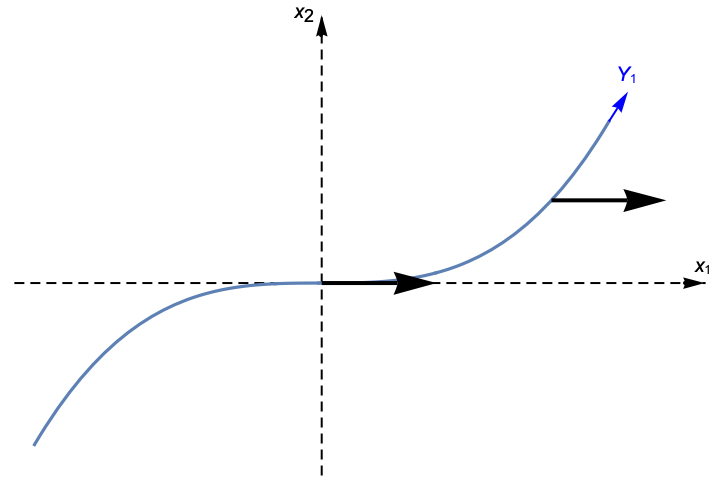
\includegraphics[width=7cm, height=5cm]{curvedaxis.png}
%    \caption{\textit{Στο επίπεδο σύστημα αναφοράς x %(διακεκομμένο) οι συνιστώσες του διανύσματος δεν μεταβάλλονται %καθώς αυτό μετακινείται, ωστόσο, στο καμπύλο σύστημα y %αλλάζουν.}}
%    \label{fig:curvedaxis}
%\end{figure}
%Η ανεπάρκεια της μερικής παραγώγου, έκδηλη από το δεύτερο όρο %της \eqref{pdertrans}, δείνει το κίνητρο για την κατασκευή της %συναλλοίωτης παραγώγου. Εκείνο που χρειαζόμαστε, είναι ένας %ακόμη όρος που να αντιπροσωπεύει τις ενδογενούς μεταβολές του %συστήματος συντεταγμένων. 
%Στο παράδειγμα του σχήματος \ref{fig:curvedaxis} ένα διάνυσμα %μετατοπίζεται παράλληλα σε έναν επίπεδο (διακεκομμένο) και έναν %καμπυλωμένο (συνεχής) χώρο με συντεταγμένες $x$ και $y$, %αντίστοιχα. Το μέτρο και η διεύθυνση του διανύσματος δεν %αλλάζει διεύθυνση, ούτε μέτρο άρα στο επίπεδο σύστημα οι %συνιστώσες του είναι σταθερές
%\begin{equation*}
%    \pd{V\superscr{\nu}}{x\superscr{\mu}} \,=\, 0
%\end{equation*}
%Λόγω της καμπυλότητας του y συστήματος όμως, οι μερικές %παραγώγοι στο εν λόγω σύστημα δεν είναι σταθερές
%\begin{equation*}
%    \pd{V'^{\nu}}{\y\superscr{\mu}} \,\neq\, 0
%\end{equation*}
\\

Επειδή η μερική παράγωγος μπορεί να είναι μηδενική σε κάποιο σύστημα αναφοράς συντεταγμένων και μη μηδενική σε κάποιο άλλο, δεν μπορεί να είναι τανυστής. Μπορούμε όμως να ορίσουμε τις συναλλοίωτες παραγώγους ανταλλοίωτων και συναλλοίωτων διανυσμάτων, οι οποίες μετασχηματίζονται ως τανυστές: 
%να εκφράσουμε τις μεταβολές συναλλοίωτου τανυστή πρώτης τάξης, %ως εξής 
\begin{equation}\label{covdevcov}
    \nabla\indices{_\mu}V\subscr{\nu} = \pd{V\subscr{\nu}}{x\superscr{\mu}} - \Gamma\indices{^\alpha_\mu_\nu} V\subscr{\alpha}
\end{equation}
ενώ για ανταλλοίωτο τανυστή πρώτης τάξης
\begin{equation}\label{covdevcont}
    \nabla\indices{_\mu}V\superscr{\nu} = \pd{V\superscr{\nu}}{x\superscr{\mu}} + \Gamma\indices{^\nu_\mu_\alpha} V\superscr{\alpha}
\end{equation}
%όπου τα πρόσιμα καθορίζονται βάση σύμβασης. Αναφερόμαστε στις %δύο πιο πάνω εκφράσεις ως η συναλλοίωτη παράγωγος, συναλλοίωτου %και ανταλλοίωτου τανυστή, αντίστοιχα. Ο δεύτερος όρος περιέχει 
Τα στοιχεία $\Gamma\indices{^\rho_\sigma_\lambda}$ ορίζονται με τέτοιο τρόπο, ώστε οι συναλλοίωτες παράγωγοι \eqref{covdevcov} και \eqref{covdevcont} να μετασχηματίζονται ως τανυστές. Για παράδειγμα,
\begin{equation*}
    \nabla\indices{_\mu}V\superscr{\nu} \rightarrow \L[i]{\alpha}{\mu}\L{\nu}{\beta}\nabla\indices{_\alpha}V\superscr{\beta}
\end{equation*}
Τα στοιχεία $\Gamma\indices{^\rho_\sigma_\lambda}$ είναι γνωστά και ως σύμβολα Christoffel. Δεν αποτελούν τις συνιστώσες κάποιου τανυστή, αφού δεν μετασχηματίζονται ανάλογα. Η γενίκευση των \eqref{covdevcov} και \eqref{covdevcont} για τανυστές μεγαλύτερης τάξης επιτυγχένεται άμεσα. Για παάδειγμα, στην περίπτωση τανυστή τέταρτης τάξης, παίρνουμε
\begin{equation*}
    \nabla\subscr{\lambda}T\indices{^\mu_\rho^\nu_\sigma} \,=\, \pd{\,}{x\superscr{\lambda}} T\indices{^\mu_\rho^\nu_\sigma}+ \Gamma\indices{^\mu_\lambda_\alpha}T\indices{^\alpha_\rho^\nu_\sigma} - \Gamma\indices{^\alpha_\lambda_\rho}T\indices{^\mu_\alpha^\nu_\sigma} + \Gamma\indices{^\nu_\lambda_\alpha}T\indices{^\mu_\rho^\alpha_\sigma} - \Gamma\indices{^\alpha_\lambda_\sigma}T\indices{^\mu_\rho^\nu_\alpha}
\end{equation*}
%---------------------------------------------------------------------------
\chapter{Βαρύτητα}
Στο κεφάλαιο αυτό εξετάζουμε τη βαρυτική δράση του Einstein και τη σύζευξη της βαρύτητας με τα ηλεκτρομαγνητικά πεδία. 
%είναι η καθολικότητα της βαρύτητας ως προς κάθε μορφή ενέργειας. 
Όλες οι μορφές ύλης και ακτινοβολίας υπόκεινται στην επίρροια της βαρύτητας. Εξάλλου, το βαρυτικό πεδίο ταυτίζεται με τον καμπυλωμένο χωρόχρονο.

\section{Η Αρχή της Ισοδυναμίας}
Στο κεφάλαιο \ref{chaptertensorcal}, αναφερθήκαμε στην αρχή της ισοδυναμίας του Einstein και αποδείξαμε ότι μια αρκετά μικρή χωροχρονική περιοχή, ανεξάρτητα από την παρουσία βαρυτικού πεδίου, μπορεί να περιγραφεί ως τμήμα του χωροχρόνου Minkowski και να επικαλυφθεί με ένα (τοπικά) αδρανειακό σύστημα αναφοράς συντεταγμένων. Ταυτόχρονα, σύμφωνα με την αρχή της ισοδυναμίας, σε μια μικρή περιοχή του χωροχρόνου, στο σύστημα αναφοράς παρατηρητή που πέφτει ελεύθερα, οι βαρυτικές δυνάμεις εξουδετερώνονται από αδρανειακές και οι νόμοι της φυσικής περιγράφονται με βάση τις αρχές της ειδικής θεωρίας της σχετικότητας. Στο τοπικά αδρνειακό σύστημα αναφοράς, η μετρική είναι η μετρική Minkowski. 
%γεωμετρία της υπόβαθρης πολλαπλότητας, πρέπει να προσεγγίζει αυτή του χωροχρόνου Minkowski
%\begin{equation*}\label{minkapprox}
%     ds^2 \approx \mink{\mu}{\nu} %dx\indices{^\mu}dx\indices{^\nu} 
%\end{equation*}
%στο προαναφερόμενο όριο. Για παράδειγμα, μια τέτοια μικρή %χωροχρονική περιοχή αντιστοιχεί σε έναν ανελκυστήρα ελεύθερο να %κινηθεί υπό την επίδραση του βαρυτικού πεδίου της γης, για %μικρό χρονικό διάστημα. Εντός του ανελκυστήρα, δύο ελεύθερα %σωματίδια τοποθετημένα στο κάτω και πάνω μέρος του ανελκυστήρα, %αφήνονται να κινηθούν στο εσωτερικό. Σύμφωνα με την αρχή, ως %προς το σύστημα αναφοράς του ανελκυστήρα, τα σωματίδια είναι %ακίνητα για ένα μικρό χρονικό διάστημα. 
Σε μεγαλύτερες περιοχές, η καμπυλότητα του χωροχρόνου και τα βαρυτικά φαινόμενα δεν μπορούν να αμεληθούν και 
%να κινείται για μεγάλους χρόνους, το σύστημα %ανελκυστήρα-σωματίδια, δεν συμπίπτει πλέον με ένα μικρό %χωροχρονικό χωρίο, και 
έτσι, γίνονται παρατηρήσιμα τα παλιρροιακά φαινόμενα. 
%Τα σωματίδια, ως προς το σύστημα του ανελκυστήρα, θα %απομακρύνονται, το ένα κινούμενο προς τα πάνω και το άλλο προς %τα κάτω. 
%\\ \\
%Τέλος, δικαιώνεται η σύντομη συζήτηση περί pseudo-Riemannian %πολλαπλότητες που έγινε στην ενότητα \ref{sec_localcartcoor}. Η %μετρική μιας πολλαπλότητας Riemann, όντας θετικά ορισμένη, δεν %μπορεί να προσεγγίσει την μετρική Minkowski με αρνητικές %ιδιοτιμές. Οδηγούμαστε λοιπόν, σε pseudo-Riemannian γεωμετρίες. %
%\begin{equation}
%    ds^2 \,=\, \g{\mu}{\nu} dx\indices{^\mu}dx\indices{^\nu} %\left\{ \begin{array}{c}
%         \le 0 \\
%         > 0
%    \end{array} \right.
%\end{equation}

\section{Δράση}
Οι εξισώσεις του Einstein στην παρουσία ηλεκτρομαγνητικών πεδίων απορρέουν από την δράση Einstein-Hilbert, $S\subscr{H}$, και τη δράση Maxwell $S\subscr{M}$ (στην απουσία φορτισμένης ύλης):
\begin{equation}\label{actionEH}
    S \,=\, S\subscr{H}\,+\,S\subscr{M} \,=\,\int \left( \frac{R}{16\pi G}-\frac{1}{4}F\subscr{\mu\nu} F\subscr{\alpha\beta}g\superscr{\mu\alpha}g\superscr{\nu\beta} \right)\sqrt{-g}\,d\superscr{4}x 
\end{equation}
Η μετρική $\g{\mu}{\nu}$, το ηλεκτρικό και το μαγνητικό πεδίο ικανοποιούν τις εξισώσεις Euler-Lagrange. Ο ηλεκτρομαγνητικός τανυστής $F\subscr{\mu\nu}$ ορίζεται ως η στροφή του ηλεκτρικού τετραδυναμικού 
\begin{equation*}
    F\subscr{\mu\nu} = \partial\subscr{\mu} A\subscr{\nu} - \partial\subscr{\nu} A\subscr{\mu}
\end{equation*}
ώστε να ικανοποιούνται οι ομογενείς εξισώσεις του Maxwell.
%με έξι ανεξάρτητα στοιχεία και μηδενική συναλλοίωτη απόκλιση %(ομογενής εξισώσεις Maxwell)
%\begin{equation*}
%    \g[i]{\rho}{\mu}\nabla\subscr{\rho} F\subscr{\mu\nu} \,=\, %0
%\end{equation*}
%Λόγω της αντισυμμετρικότητας του $F\subscr{\mu\nu}$, η %αντικατάσταση των μερικών παραγώγων με συναλλοίωτες παραγώγους %-όπως απαιτεί, άλλωστε, η αναγωγή τανυστικών εξισώσεων από %ειδική σε γενική σχετικότητα- δεν αλλάζει τη μορφή του.

\section{Μεταβολή δράσης}
%Η γεωμετρία του χωροχρόνου καθορίζεται, βελτιστοποιώντας το %συναρτησιακό \eqref{actionEH} ως προς τη μετρική %$\g{\mu}{\nu}$. 
Μια απειροστά μικρή μεταβολή της μετρικής 
\begin{equation*}
    \g{\mu}{\nu} \rightarrow \g{\mu}{\nu}\,+\,\de\g{\mu}{\nu}
\end{equation*}
μεταβάλλει τη δράση κατά
\begin{equation}\label{actionvar}
    \de\subscr{g} S \,=\, \de\subscr{g} S\subscr{H} \,+\, \de\subscr{g} S\subscr{M}
\end{equation}
%όπου ο δείχτης g υποδεικνύει την εν λόγο μεταβολή έναντι άλλων %μεταβολών όπως, παραδείγματος χάριν, αυτήν ως προς το δυναμικό %βαθμίδος $A\superscr{\mu}$. Ο δείχτης θα παραλειφθεί στα %ακόλουθα για αποφυγή συνοστισμού. 
Ο πρώτος όρος της \eqref{actionvar} ισούται με
\begin{equation}
    \de S\subscr{H} \,=\, \int\left( \de g\superscr{\mu\nu}R\subscr{\mu\nu}\sqrt{-g} \,+\,  g\superscr{\mu\nu}\de R\subscr{\mu\nu}\sqrt{-g} \,+\, g\superscr{\mu\nu}R\subscr{\mu\nu}\de \sqrt{-g}\right)\,d\superscr{4}x 
\end{equation}
Στο παράρτημα \ref{EHvar} δείχνουμε ότι 
\begin{equation*}
    \de S\subscr{H} \,=\, \int\left( \frac{\R{\mu}{\nu} - \frac{1}{2}R\g{\mu}{\nu}}{16\pi G} \right)\, \de \g[i]{\mu}{\nu}\,\sqrt{-g}\,d\superscr{4}x 
\end{equation*}
Μεταβάλλοντας τη δράση Maxwell, ακολουθώντας τα σχετικά βήματα του παραρτήματος \ref{Maxwvar}, παίρνουμε
\begin{equation*}
    \de S\subscr{M} \,=\, \int\left( -\frac{1}{2}F\subscr{\mu\alpha} F\subscr{\nu\beta}\g[i]{\alpha}{\beta} + \frac{1}{8}F^2 \g{\mu}{\nu} \right)\, \de \g[i]{\mu}{\nu}\,\sqrt{-g}\,d\superscr{4}x 
\end{equation*}
%Ακολουθώντας το λογισμό μεταβολών, η βελτιστοποίηση του %συναρτησιακού της δράσης απαιτεί 
Απαιτώντας η δράση να είναι οριακή,
\begin{equation*}
    \frac{1}{\sqrt{-g}}\frac{\de S}{\de \g[i]{\mu}{\nu}} \,=\, 0
\end{equation*}
καταλήγουμε στις εξισώσεις Euler-Lagrange, ή στις εξισώσεις Einstein, για τη μετρική
\begin{equation}\label{elequations}
    \R{\mu}{\nu} - \frac{1}{2}R\g{\mu}{\nu} \,=\, 8\pi G\left(F\subscr{\mu\alpha} F\subscr{\nu\beta}\g[i]{\alpha}{\beta} - \frac{1}{4}F^2 \g{\mu}{\nu} \right)
\end{equation}

\section{Βαρυτικές Εξισώσεις}
Στο δεξιό μέλος της \eqref{elequations} εμφανίζεται ο τανυστής ενέργειας-ορμής, $T\subscr{\mu\nu}$, των ηλεκτρομαγνητικών πεδίων 
\begin{equation}\label{energy_mom_tensor}
    T\subscr{\mu\nu} \,:=\, F\subscr{\mu\alpha} F\subscr{\nu\beta}\g[i]{\alpha}{\beta} - \frac{1}{4}F^2 \g{\mu}{\nu}
\end{equation}
ο οποίος έχει μηδενική συναλλοίωτη απόκλιση
\begin{equation*}
    \g[i]{\rho}{\mu}\nabla\subscr{\rho}T\subscr{\mu\nu} \,=\, 0
\end{equation*}
Στη συνέχεια, βρίσκουμε το ίχνος των δύο μελών της εξίσωσης Einstein, πολλαπλασιάζοντας με τον αντίστροφο της μετρικής $\g[i]{\mu}{\nu}$ και χρησιμοποιώντας τη σχέση $\g[i]{\mu}{\nu}\g{\mu}{\nu}=4$. Με βάση το αποτέλεσμα $R=-8\pi G T$, οι βαρυτικές εξισώσεις του Einstein ανάγονται στην ακόλουθη βοηθητική μορφή
\begin{equation}\label{einstein equations}
    \R{\mu}{\nu} \,=\, 8\pi G\left( T\subscr{\mu\nu} -\frac{1}{2}T\g{\mu}{\nu} \right)
\end{equation}
Στην απουσία φορτισμένης ύλης το ίχνος του τανυστή της ενέργειας-ορμής των ηλεκτρομαγνητικών πεδίων μηδενίζεται και έτσι
\begin{equation}
    \R{\mu}{\nu} \,=\, 8\pi G T\subscr{\mu\nu} 
\end{equation}
%\newpage

Οι λύσεις των βαρυτικών εξισώσεων στην παρουσία ηλεκτρομαγνητικών πεδίων προσδιορίζουν τις $10$ ανεξάρτητες συνιστώσες του μετρικού τανυστή $\g{\mu}{\nu}$.


\section{Στατικές και σφαιρικά συμμετρικές λύσεις}
θα βρούμε στατικές και σφαιρικά συμμετρικές λύσεις. 
%που να είναι, πρώτον στατικές, αμετάβλητες δηλαδή ως προς %χρονικές μετατοπίσεις και αναστροφές. 
Έτσι, κάθε στοιχείο της μετρικής πρέπει να είναι ανεξάρτητο της χρονικής συντετραγμένης, και θέτουμε 
%η μορφή της μετρικής περιορίζεται με το μηδενισμό των όρων 
\begin{equation*}
\g{0}{1},\,\g{0}{2},\,\dots\,=\,0
\end{equation*}
Η χρονική συνιστώσα της μετρικής, $\g{0}{0}$, είναι διάφορη από μηδέν. 
%Τα σύνολα των σημείων του χωροχρόνου με σταθερή χρονική και %ακτινική συνιστώσα καθορίζονται από τις πολικές συντεταγμένες %(θ,φ) και συνιστούν 2-σφαίρες στον τρισδιάστατο χώρο. Οι %2-σφαίρες είναι συμμετρικές ως προς χωρικές περιστροφές. Αυτή η %ιδιότητα, οδηγεί στον μηδενισμό όρων με συνδυασμούς των χωρικών %συντεταγμένων
%\begin{equation*}
%    \g{1}{2},\,\g{2}{3},\,\dots\,=\,0
%\end{equation*}
Χρησιμοποιώντας σφαιρικές συντεταγμένες για το χώρο, μπορεί να αποδειχθεί ότι η πιο γενική, σφαιρικά συμμετρική μετρική παίρνει την ακόλουθη μορφή \cite{Weinberg:100595}: 
%γίνεται λεπτομερής μελέτη χωροχρόνων με υποχώρους πλήρης %συμμετρικότητας και αποδεικνύονται τα πάραπάνω. Τα στοιχεία της %μετρικής που επιβιώνουν τους παραπάνω περιορισμούς είναι τα %διαγώνια. Παραλείποντας τις εξειγήσεις που δείνει στο βιβλίο %του ο Weinberg καταλήγουμε στην μετρική
\begin{equation}\label{metric_first_form}
    ds^2 \,=\, -e^{2a(r)}\,dt^2 \,+\, e^{2b(r)}\,dr^2 \,+\, r^2\,(d\theta^2 + \sin\superscr{2}\theta\,d\phi^2)
\end{equation}
%Είναι βοηθητικό αλλά όχι απαραίτητο να επιβάλουμε οι a και b να %είναι θετικές περιορίζοντας τις σε εκθετικές συναρτήσεις της r. Έτσι, διατηρείται η ταυτότητα της μετρικής, (-+++)
%\begin{equation}
%    g\subscr{\mu\nu}\,:=\,diag\left(-e^{2a(r)},\,e^{2b(r)},\,r^%2,\,r^2\sin\superscr{2}\theta\right)
%\end{equation}
%Λόγω του μεγάλου όγκου πράξεων, 
Οι υπολογισμοί γίνονται με τη βοήθεια του λογισμικού Wolfram Mathematica και παρουσιάζοναι στο παράρτημα \ref{mathematica}. Στον κώδικα \ref{mathematica_position_n_metric} ορίζουμε τη μετρικής σύμφωνα με την \eqref{metric_first_form}, στις συντεταγμένες $x\superscr{\mu}=(t,r,\theta,\phi)$. Στη συνέχεια, προσδιορίζουμε τα σύμβολα Christoffel (κώδικας \ref{mathematica_chr_symbols})
\begin{equation}\label{christoffel symbols identity}
    \Gamma\indices{^\sigma_\mu_\nu} \,=\, \frac{1}{2}\g[i]{\sigma}{\rho}\left( \partial\subscr{\mu}\g{\nu}{\rho} + \partial\subscr{\nu}\g{\rho}{\mu} - \partial\subscr{\rho}\g{\mu}{\nu} \right)
\end{equation}
Έχοντας βρει τα στοιχεία της σύνδεσης, προσδιορίζουμε τον τανυστή καμπυλότητας Riemann με βάση τη σχέση 
\begin{equation}
    \R[\rho]{\mu}[\lambda]{\nu} \,=\, \partial\subscr{\lambda}\Gamma\superscr{\rho}\subscr{\;\;\mu\nu} \,+\, \Gamma\superscr{\rho}\subscr{\;\;\lambda\sigma}\Gamma\superscr{\sigma}\subscr{\;\;\mu\nu} \,-\, \partial\subscr{\nu}\Gamma\superscr{\rho}\subscr{\;\;\mu\lambda} \,-\, \Gamma\superscr{\rho}\subscr{\;\;\nu\sigma}\Gamma\superscr{\sigma}\subscr{\;\;\mu\lambda}
\end{equation}
τρέχοντας τον κώδικα \ref{mathematica_Riemann}. Στις εξισώσεις Einstein εμπλέκεται ο τανυστής Ricci, ο οποίος αποτελεί ίχνος του τανυστή Riemann, κώδικας \ref{mathematica_Ricci}
\begin{equation}
    \R{\mu}{\nu}\,:=\,\R[\lambda]{\mu}[\lambda]{\nu}
\end{equation}
Στη συνέχεια βρίσκουμε τον ηλεκτρομαγνητικού τανυστή και τον τανυστή ενέργειας-ορμής \eqref{energy_mom_tensor}.

\section{Ηλεκτρομαγνητικός τανυστής}
Στη διατριβή αυτή θα μελετήσουμε μαγνητικά φορτισμένες μελανές οπές και διάφορα φυσικά φαινόμενα που συνδέονται με αυτές \cite{Maldacena_2021}. Ο ηλεκτρομαγνητικός τανυστής πρέπει να περιγράφει το ακτινικό μαγνητικό πεδίο μαγνητικού μονοπόλου. Το μαγνητικό φορτίο είναι κβαντωμένο με βάση τη συνθήκη κβάντωσης Dirac \eqref{quantum magnetic charge}. Στην εξωτερική περιοχή του ορίζοντα, έχει την ακόλουθη διανυσματική μορφή 
\begin{equation*}
    \vec{B} \,=\, \frac{q\subscr{m}\vec{r}}{r\superscr{3}}
\end{equation*}
Αντικαθιστούμε το φορτίο $q\subscr{m}$ με ακέραιο πολλαπλάσιο του στοιχειώδους μαγνητικού κβάντου\footnote{Στις μονάδες Planck θέτουμε $\hbar=c=1$}, \eqref{quantum magnetic charge}, και έχουμε
\begin{equation*}
    \vec{B}\,=\,\frac{Q\vec{r}}{2er^3}
\end{equation*}
Η συνολική μαγνητική ροή ισούται με
\begin{equation*}
    \oint\vec{B}\cdot d\vec{s} = \frac{2\pi}{e}Q
\end{equation*}
Με χρήση της σχέσης \cite{Carroll2003-CARSAG-3}  
\begin{equation}
    B\superscr{r}=\epsilon\superscr{tr\mu\nu}F\subscr{\mu\nu}=\frac{\epsilon\superscr{rjk}}{\sqrt{-g}}F\subscr{jk}
\end{equation}
βρίσκουμε τα μη μηδενικά στοιχεία του ηλεκτρομαγνητικού τανυστή $F\subscr{\mu\nu}$
\begin{equation}\label{def of em tensor}
    \begin{split}
        &F\subscr{0i} \,=\, 0\\
        &F\subscr{jk} \,=\, -F\subscr{kj} \,=\,\left\{\begin{array}{c}
             \frac{Q}{2e}\sin\theta,\quad \text{\scalebox{0.7}{$j=\theta,\,\,k=\phi $}} \\
             0,\quad \text{\scalebox{0.7}{ υπόλοιπα}}
        \end{array} \right.
    \end{split}
\end{equation}

Έχοντας λοιπόν, τον τανυστή \eqref{def of em tensor}, προσδιορίζουμε τον τανυστή της ενέργειας - ορμής \eqref{energy_mom_tensor}, κώδικας \ref{mathematica energy momentum tensor}. 

%Βρίσκουμε στη συνέχεια το ίχνος Τ του τανυστή ενέργειας-ορμής %με τον κώδικα \ref{mathematica trace of ene mom ten} και τέλος %κατασκευάζουμε το δεξιό μέλος της \ref{einstein equations}, %κώδικας \ref{mathematica rs of einstein eq}. Το %ηλεκτρομαγνητικό πεδίο, που θα χρησιμοποιηθεί στο κβαντικό %πλαίσιο της ενότητας \ref{section dirac equation in gravity}, %δίνεται από τη συνιστώσα $A\subscr{\phi}$
%\begin{equation}\label{vector potential for monopole in %curvilinear coo}
%    A\subscr{\phi}=\frac{Q}{2e}\cos\theta
%\end{equation}

\section{Λύσεις εξισώσεων Einstein}
Έχουμε στην κατοχή μας όλα τα τανυστικά μεγήθη για να καταστρώσουμε τις εξισώσεις του Einstein \eqref{einstein equations}. Καταλήγουμε σε ένα σύστημα τεσσάρων εξισώσεων, που παρουσιάζονται τρέχοντας τον κώδικα \ref{mathematica system of einstein equations}. Υπάρχει μία εξίσωση δηλαδή για κάθε διαγώνιο στοιχείο του τανυστή Ricci   
\begin{equation}
    \begin{split}
        &\{tt\}\,:\quad -e^{2b}A + r\superscr{3}\left( a'(2+ra'-rb')+ra'' \right)\,=\,0\\
        &\{rr\}\,:\quad e^{2b}A + r\superscr{3}\left( 2b'+a'(-ra'+rb')-ra'' \right) \,=\,0 \\
        &\{\phi\phi\}\,:\quad  1 - \frac{A}{r^2} - e^{-2b}\left( 1 + ra' -rb' \right) = 0\\
        &\{\theta\theta\}\,:\quad \{ \phi\phi \}
    \end{split}
\end{equation}
όπου $A=\frac{G\pi Q^2}{e^2}$. Προσθέτουμε τις tt και rr εξισώσει, και παίρνουμε τη σχέση a' = -b'. Στη συνέχεια αντικαθιστούμε στην εξίσωση θθ και καταλήγουμε στην ακόλουθη διαφορική εξίσωση 
\begin{equation}\label{differential equation for metric components}
    2r\frac{db}{dr}+e^{2b}(1-\frac{A}{r\superscr{2}})-1=0
\end{equation}
Η λύση της \eqref{differential equation for metric components} παρουσιάζεται στο παράρτημα \ref{solution for metric dif eq}. Το αποτέλεσμα είναι 
\begin{equation}
    b(r) \,=\, -\frac{1}{2}\ln{\left(1-\frac{2G\pi Q^2}{e^2r}c+\frac{G\pi Q^2}{e^2r^2}\right)}
\end{equation}
όπου $c$ σταθερά, ανεξάρτητη της ακτινικής συντεταγμένης $r$. Για να βρούμε τη σταθερά αυτή, απαιτούμε να αναπαράγεται η μετρική Schwarzschild για μηδενικό αγνητικό φορτίο: 
\begin{equation*}
    Q\rightarrow 0 \quad \Rightarrow \quad \left(1-\frac{2G\pi Q^2}{e^2r}c+\frac{G\pi Q^2}{e^2r^2}\right)\rightarrow \left(1-\frac{2GM}{r}\right)\quad\Rightarrow \quad c=\frac{M e^2}{\pi Q^2 }
\end{equation*}
όπου $M$ η μάζα της μαύρης τρύπας.
Με βάση τα πιο πάνω, καταλήγουμε στην μετρική Reissner-Nordström, με μη μηδενικό μαγνητικό φορτίο $Q$
\begin{equation}\label{ReissnerNordmetric}
    ds^2 \,=\, -B\,dt^2\,+\,B^{-1}\,dr^2+r^2\,d\Omega^2, \quad B(r)=1-\frac{2G M}{r}+\frac{G\pi Q^2}{e^2r^2}
\end{equation}


\section{Μελανές Οπές Reissner-Nordström}
Στη μετρική \eqref{ReissnerNordmetric}, τα αντίθετα πρόσημα των δύο τελευταίων όρων οδηγούν σε ενδιαφέροντα χαρακτηριστικά. Πρώτον, υπάρχουν γενικά δύο ορίζοντες 
%(έναντι του ενός στην περίπτωση της γεωμετρίας Schwarzschild) 
στις ακτίνες
\begin{equation}\label{horizon radius}
    r_{\pm} = GM\left[1\pm\sqrt{1 - \frac{\pi Q^2}{Ge^2M^2}}\right]
\end{equation}
Δεύτερον, ο όρος της μάζας επιδρά διαφορετικά στη γεωμετρία της περιοχής του ορίζοντα σε σχέση με τον όρο του φορτίου εξαιτίας του αντίθετου προσήμου. Στον πίνακα \ref{table:mass to charge ratio} συνοψίζονται τα χαρακτηριστικά των ακόλουθων τριών ειδών φορτισμένων μελανής οπών. 
%- περίσσεια φορτίου έναντι μάζας, περίσσεια μάζας έναντι %φορτίου και ισότητα. 
Στη πρώτη περίπτωση, $GM^2<\pi Q^2/e^2$, εκδηλώνεται γυμνή ανωμαλία και περιοχές με μεγάλη καμπυλότητα, οι οποίες δεν μπορούν να περιγραφούν με βάση την κλασική θεωρία του Einstein για τη βαρύτητα. 
%αν και φυσικά σωστή, π.χ. το ηλεκτρόνιο, δεν περιγράφεται από %τη κλασική σχετικότητα. \\
Στη δεύτερη περίπτωση, $GM^2>\pi Q^2/e^2$, υπάρχουν δύο ορίζοντες σε ακτίνες $r\subscr{+}$ και $r\subscr{-}<r\subscr{+}$. Οι λύσεις αυτές εξετάζονται στη συνέχεια, και διερευνούμε την εξωτερική περιοχή κοντά στον ορίζοντα $r_+$. Η τρίτη περίπτωση, αφορά τις ακραίες μαύρες τρύπες οι οποίες ικανοποιούν την ισότητα $GM^2=\pi Q^2/e^2$. Στην περίπτωση αυτή οι δύο ορίζοντες ταυτίζονται $r\subscr{+}=r\subscr{-}$.

\begin{table}[t]
    \centering
    \begin{tabular}{|p{4.5cm}|p{4.5cm}|p{4.5cm}|}
            \hline
            $GM^2 < \pi Q^2/e^2$ & $GM^2 > \pi Q^2/e^2$ & $GM^2 = \pi Q^2/e^2$\\
            \hline
            Γυμνή ανομαλία & Ορίζοντες στα $r_{\pm}$ & Ορίζοντας στο $r=r\subscr{e}\equiv GM$\\
            $r$ πάντα χωροειδής & $r_-<r<r_+ \rightarrow$ $r$ χρονοειδής & $r$ πάντα χωροειδής \\
            Χρονοειδείς τροχιές μπορούν να αποφύγουν την ανομαλία & $r<r_-\rightarrow$ $r$ χωροειδής & \\
            \hline
    \end{tabular}
    \caption{\textit{Χαρακτηριστικά φορτισμένων μελανών οπών με βάση το πηλίκο της μάζας προς το φορτίο.}}
    \label{table:mass to charge ratio}
\end{table}

%\newpage
\section{Θερμοκρασία Hawking φορτισμένων οπών}
Τα θερμοδυναμικά χαρακτηριστικά των φορτισμένων μελανών οπών εξάγονται με βάση τις αρχές της γενικής σχετικότητας και της κβαντομηχανικής \cite{Susskind:2005js}. Κοντά στον ορίζοντα $r\subscr{+}$, η 
ακτινική απόσταση ρ σημείου $r$ της εξωτερικής περιοχής από τον ορίζοντα δίδεται από τη σχέση 
%ελαφρώς μεγαλύτερο από $r\subscr{+}$ είναι
\begin{equation}
    \rho = \int\limits_{r\subscr{+}}^r \frac{r'dr'}{\sqrt{(r-r\subscr{+})(r-r\subscr{-})}}\approx 2r\subscr{+}\sqrt{\frac{r-r\subscr{+}}{r\subscr{+}-r\subscr{-}}}
\end{equation}
Αντικαθιστώντας στην \eqref{ReissnerNordmetric}, βρίσκουμε ότι η μετρική κοντά στον ορίζοντα $r\subscr{+}$ προσεγγίζεται από τη μετρική Rindler
\begin{equation}\label{rindler metric close to horizon}
    ds^2\approx -\rho^2 d\omega^2\,+\,d\rho^2 + r\subscr{+}^2 d\Omega^2 \quad\quad \omega\equiv\frac{r\subscr{+}-r\subscr{-}}{2r\subscr{+}^2}t
\end{equation}
Με τον ακόλουθο μετασχηματισμό συντεταγμένων
\begin{equation}\label{coordinate tran from rindler to minkowski}
    T=\rho\sinh{\omega}\qquad Z=\rho\cosh{\omega}\qquad X=r\subscr{+}\theta\cos\phi \qquad Y=r\subscr{+}\theta\sin\phi
\end{equation}
κοντά στο σημείο $\theta = 0$, επιτυγχάνουμε τη μετάβαση στο τοπικά ορισμένο αδρανειακό σύστημα συντεταγμένων $(T,\,Z,\,X,\,Y)$, κατάλληλο για να περιγράψει τις παρατηρήσεις ενός παρατηρητή που πέφτει ελεύθερα κοντά στον ορίζοντα $r\subscr{+}$. 
%με τον Z άξονα του προσανατολισμένο ακτινικά στο $\theta=0$. 
Σύμφωνα με την αρχή της ισοδυναμίας, ο μετασχηματισμός \eqref{coordinate tran from rindler to minkowski} αποτελεί το βαρυτικό ισοδύναμο της σχέσης μεταξύ ενός αδρανειακού συστήματος αναφοράς (στην απουσία βαρυτικού πεδίου) και ενός επιταχυνόμενου συστήματος αναφοράς, με σταθερή ομοιόμορφη επιτάχυνση. Ο παρατηρητής Schwarzschild διαγράφει υπερβολοειδή τροχιά από τη σκοπιά του παρατηρητή που πέφτει ελεύθερα.\\ 

Σύμφωνα με το φαινόμενο Unruh, ο παρατηρητής Schwarzschild ανιχνεύει μια θερμική ατμόσφαιρα, με θερμοκρασία
\begin{equation}
    T(r{\scriptscriptstyle\gtrsim} r\subscr{+})\,=\,\frac{1}{2\pi}\frac{1}{\rho(r)}
\end{equation}
%Επικαλώντας και πάλι την αρχή της ισοδυναμίας, το φαινόμενο %Unruh αναθέτει θερμικό περιβάλλον στον μη αδρανειακό παρατηρητή %που βρίσκεται στάσιμος κοντά στον ορίζοντα της οπής. 
Αρκετά μακριά από την μελανή οπή, η θερμοκρασία έχει σταθερή τιμή και ισούται με τη θερμοκρασία Hawking: 
%Λόγω της διαστολής της χρονικής συντεταγμένης και της %αντίστοιχης ερυθρής μετατόπισης της συχνότητας $\nu\subscr{t}$ %των κβάντων ακτινοβολίας γύρω από την οπή (όπου t ο χρόνος %Schwarzschild)
%\begin{equation*}
%    \omega\,=\,\frac{r\subscr{+}-r\subscr{-}}{2r\subscr{+}^2}t %\quad\Rightarrow\quad %\nu\subscr{t}\,=\,\frac{r\subscr{+}-r\subscr{-}}{2r\subscr{+}^2%}\nu\subscr{\omega}
%\end{equation*}
%η θερμοκρασία Hawking είναι
\begin{equation}\label{temp of black hole at a distance}
    T(r\rightarrow\infty)\,=\,\frac{1}{2\pi}\frac{r\subscr{+}-r\subscr{-}}{2r\subscr{+}^2}
\end{equation}
Ένας στάσιμος παρατηρητής ατο άπειρο αντιλαμβάνεται τη μελανή οπή ως ένα μέλαν σώμα, με θερμοκρασία 
%που δίνεται από την 
\eqref{temp of black hole at a distance}. Στο όριο μιας ακραίας φορτισμένης οπής, οι δύο ορίζοντες $r\subscr{+}$ και $r\subscr{-}$ ταυτίζονται και η θερμοκρασία Hawking  μηδενίζεται. 

\section{Μικρές αποκλίσεις από την ακραία μελανή οπή}
Στο όριο $M\rightarrow \frac{\pi Q\superscr{2}}{Ge\superscr{2}}$, η θερμοκρασία τείνει στο μηδέν και η ακτινοβολία Hawking καταστέλλεται. Για μικρές αποκλίσεις της μάζας, αναμένεται αύξηση της θερμοκρασίας, και η οπή αρχίζει να ακτινοβολεί μέχρι που η μάζα να ελαττωθεί στην οριακή της τιμή. Για μικρές μεταβολές της μάζας, διατηρώντας το φορτίο σταθερό,
\begin{equation}
    M\subscr{e}\rightarrow M = M\subscr{e}+\de M,\qquad \de M << M\subscr{e}\superscr{2} = \pi Q^2/Ge^2
\end{equation}
παίρνουμε για την ακτίνα του εξωτερικού ορίζοντα $r\subscr{+}$ \eqref{horizon radius} 
\begin{equation}
    r\subscr{+} = GM\left[ 1+\sqrt{1-\frac{M\subscr{e}\superscr{2}}{M\superscr{2}}} \right]\quad \approx\quad GM\left[ 1+\sqrt{2\frac{\de M}{M\subscr{e}}} \right]
\end{equation}
και τη θερμοκρασία Hawking 
\begin{equation}
    T = \frac{1}{2\pi GM\subscr{e}}\sqrt{\frac{\de M}{M\subscr{e}}}\,+\,\mathcal{O}\left( \frac{\de M}{M\subscr{e}}\right)
\end{equation}
Η μεταβολή της μάζας 
%που θα "ακτινοβοληθεί" παραμετρικοποιείται ακολούθως 
δίδεται συναρτήσει της θερμοκρασίας της μελανής οπής από τη σχέση
\begin{equation}\label{small mass above extremality in terms of temperature}
    \de M \sim \frac{2\pi\superscr{\frac{7}{2}}G\superscr{\frac{1}{2}}Q\superscr{3}}{e\superscr{3}}T\superscr{2}
\end{equation}
%Στην πραγματικότητα, η οπή δεν χάνει μάζα μόνο υπό τη μορφή %ακτινοβολίας αλλά, 
'Οπως θα δούμε στη συνέχεια, η εξαΰλωση της μελανής οπής ενισχύεται όταν η ένταση του μαγνητικού πεδίου στην περιοχή του ορίζοντα υπερβεί μια οριακή τιμή που καθορίζεται από τη μάζα του μποζονίου Higgs.
%από άμαζα φερμιόνια, δεδομένου ότι το μαγνητικό πεδίο στο %εξωτερικό έχει ένταση $|F|$ μεγαλύτερο του κατώτατου ορίου %$m\subscr{h}\superscr{2}$ (μάζα μποζονίου Higgs).

%---------------------------------------------------------------------------
\chapter{Σφαιρικό πρόβλημα Landau}
%Η θερμική ατμόσφαιρα του ορίζοντα μιας μη φορτισμένης μελανής %οπής, αποτέλεσμα κβαντικών διακυμάνσεων του κενού, μεταφέρεται %στο άπειρο υπό τη μορφή ακτινοβολίας Hawking. 
Στην παρουσία ισχυρού μαγνητικού πεδίου, πέραν της ακτινοβολίας Hawking, αναμένεται να εκδηλωθούν φαινόμενα όπως η δίδυμος γένεση φερμιονίων-αντιφερμιονίων. Επομένως, χρειάζεται να μελετήσουμε φερμιονικά πεδία στην παρουσία πεδίου μαγνητικού μονοπόλου. Θα μελετήσουμε πρώτα το μη σχετικιστικό πρόβλημα, ενός φορτισμένου σωματιδίου στην παρουσία ενός τέτοιου μαγνητικού πεδίου, ακολουθώντας την εργασία του Haldane \cite{PhysRevLett.51.605}. 
%ο Haldane αναπτύσσει τις μη-σχετικιστικές, μονοσωματιδιακές %συναρτήσεις εντοπισμένες σε σφαιρική επιφάνεια ομόκεντρη με %μαγνητικό μονόπολο και καταλήγει στην κβάντωση του συστήματος %στα επίπεδα Landau, κάθε ένα από τα οποία αντιστοιχεί σε μια %ιδιοτιμή της ενέργειας.

\section{Σφαιρικές λύσεις στην απουσία μαγνητικού μονοπόλου}
Η χαμιλτονιανή ελέυθερου, μη σχετικιστικού σωματιδίου είναι 
\begin{equation}
    H \,=\, \frac{\Vec{p}\superscr{\,2}}{2m}
\end{equation}
με τον τελεστή της ορμής να δίδεται από τη σχέση 
\begin{equation*}
\begin{split}
    &\Vec{p}\,\equiv\,-i\hbar\vec{\nabla}\\
    &\left[ H, \Vec{p} \right]\,=\,0
\end{split}
\end{equation*}
Οι στάσιμες, χωριζόμενες λύσεις της εξίσωσης Schrödinger είναι 
\begin{equation}
    \psi\text{\scalebox{0.7}{($r,\,t$)}}\sim e\superscr{\frac{i}{\hbar}(p\cdot r - Et)}
\end{equation}
όπου $p$ το μέτρο της ορμής και $E=\frac{p^2}{2m}$ η τιμή της ενέργειας (ή η αντίστοιχη ιδιοτιμή της χαμιλτονιανής).\\

Θα επιβάλουμε τώρα, το σωματίδιο να κινείται στην επιφάνεια μιας σφαίρας. Η χαμιλτονιανή μπορεί να γραφεί 
%στην πιο βοηθητική μορφή, 
συναρτήσει της στροφορμής, η οποία διατηρείται σταθερή 
\begin{equation}\label{angular momentum operator}
    \Lambda\superscr{i} \,=\, \epsilon\superscr{ijk}r\superscr{j}p\superscr{k}
\end{equation}
Χρησιμοποιώντας την ταυτότητα $\epsilon\superscr{ijk}\epsilon\superscr{mnk}=\de\superscr{im}\de\superscr{jn}-\de\superscr{in}\de\superscr{jm}$ και τον μεταθέτη $[r\superscr{i},p\superscr{j}]\,=\,i\hbar\de\superscr{ij}$ βρίσκουμε τη στροφορμή στο τετράγωνο
\begin{equation*}
    \Vec{\Lambda}\superscr{2}\,=\,r\superscr{2}p\superscr{2}+i\hbar\,\Vec{r}\cdot\Vec{p}-(\Vec{r}\cdot\Vec{p})\superscr{2}
\end{equation*}
Σημειώνουμε ότι το διάνυσμα θέσης είναι πάντα κάθετο στην ορμή (κίνηση κατά μήκος σφαιρικής επιφάνειας) και έτσι καταλήγουμε  στη σχέση
\begin{equation}
    \Vec{r}\cdot\Vec{p}\,=\,0\,\,\Rightarrow\,\, p\superscr{2}=\frac{\Lambda\superscr{2}}{r\superscr{2}}
\end{equation}
Συνεπώς, η χαμιλτονιανή γράφεται
\begin{equation}
    H\,=\,\frac{|\Lambda|\superscr{2}}{2mr\superscr{2}}
\end{equation}
Επειδή ο μεταθέτης
\begin{equation*}
    \left[ H,\,\Vec{\Lambda} \right] \,=\, 0
\end{equation*}
μηδενίζεται, η στροφορμή $\Vec{\Lambda}$ διατηρείται. Οι συνιστώσες της στροφορμής \eqref{angular momentum operator} ικανοποιούν την $SU(2)$ άλγεβρα των περιστροφών 
\begin{equation}
    [\Lambda\superscr{i},\Lambda\superscr{j}]\,=\,i\epsilon\superscr{ijk}\Lambda\superscr{k}
\end{equation}
Η στροφορμή στο τετράγωνο είναι κβαντισμένη με ιδιοτιμές
\begin{equation}\label{eigenvalues of L squared}
    |\Vec{\Lambda}|^2\,=\,\hbar^2\,\ell(\ell+1)\quad\,\,\ell=0,1,2,\dots
\end{equation}
Οι αντίστοιχες ιδιοσυναρτήσεις  
%\eqref{eigenvalues of L squared}, την ορθοκανονική βάση των
είναι οι σφαιρικές αρμονικές
\begin{equation}
\begin{split}
    &\Lambda\superscr{2}\,\,Y\superscr{m}\subscr{\ell}\text{\scalebox{0.7}{$(\theta,\phi)$}}\,=\,\hbar\ell(\ell+1)\,\,Y\superscr{m}\subscr{\ell}\qquad \ell\,=\,0,1,2,\dots\\
    &\Lambda\subscr{z}\,\,Y\subscr{\ell}\superscr{m}\text{\scalebox{0.7}{$(\theta,\phi)$}}\,=\,\hbar m\,\,Y\subscr{\ell}\superscr{m}\qquad -\ell\le m \le\ell
\end{split}
\end{equation}
οι οποίες απαρτίζουν μια πλήρη ορθοκανονική βάση. Με βάση τις σφαιρικές αρμονικές βρίσκουμε τις στάσιμες, χωριζόμενες λύσεις της εξίσωσης Schrodinger.
Η κατάσταση ελάχιστης ενέργειας 
%προκύπτει για $\ell = 0$ με τη 
είναι η σφαιρικά συμμετρική αρμονική $Y\superscr{o}\subscr{o}=\frac{1}{2}\frac{1}{\sqrt{\pi}}$. 
%Ο γενικός εκφυλισμός των ιδιοτιμών εξαφανίζεται στη %συγκεκριμένη περίπτωση, μια σημαντική διαφορά με την περίπτωση %του κεντρικού μαγνητικού πεδίου που εξετάζεται στην επόμενη %ενότητα.

\section{Σφαιρικές λύσεις στην παρουσία μαγνητικού μονοπόλου}
Το πεδίο του μαγνητικού μονοπόλου δίδεται από τη σχέση
%καθορίζεται από την \eqref{centralB} σε συνδυασμό με την %κβάντωση Dirac $q\subscr{m}\,=\,\frac{\hbar}{2e}$ (c=1)
\begin{equation}\label{radial magnetic field}
    \Vec{B}\,=\,\frac{\hbar s\subscr{0}}{e r^2}\,\hat{\Omega} \qquad\,\,\hat{\Omega}\,=\,\frac{\Vec{r}}{r}
\end{equation}
όπου $2s\subscr{0}$ ο λόγος της συνολικής μαγνητικής ροής προς τη στοιχειώδη μαγνητική ροή $\Phi_0$
\begin{equation}
    \frac{\Phi}{\Phi\subscr{0}}\,=\,2 s\subscr{0} \qquad s\subscr{o}=1,2,\dots
\end{equation}
Η στοιχειώδης μαγνητική ροή ισούται με
\begin{equation}
    \Phi\subscr{0}\,=\,4\pi R^2B\subscr{0}\,=\,\frac{2\pi\hbar}{e}
\end{equation}
Η χαμιλτονιανή ενός μη σχετικιστικού ηλεκτρονίου, με αρνητικό φορτίο $-e$, το οποίο αλληλεπιδρά με διανυσματικό δυναμικό $\vec{A}$, η στροφή του οποίου παράγει το μαγνητικό πεδίο 
\begin{equation*}
    \epsilon\superscr{ijk}\nabla\superscr{j}A\superscr{k}\,=\,|\Vec{B}|\,\Omega\superscr{i}\qquad i,j,k=\{x,\y,z\}
\end{equation*}
ισούται με
\begin{equation*}
    H\,=\,\frac{1}{2m}\left( \Vec{p} + e\Vec{A} \right)^2 
\end{equation*}
%όπου $\Vec{p} = -i\hbar\nabla$ ο γεννήτορας μεταθέσεων και
Ο τελεστής $\Vec{\text{Π}}\equiv\Vec{p}+e\Vec{A}$ είναι η μηχανική ορμή του ηλεκτρονίου \cite{Sakurai:1167961}. Γενικά για ένα σωματίδιο με αρνητικό φορτίο $-q$, οι συνιστώσες του τελεστή της μηχανικής ορμής ικανοποιούν τις ακόλουθες σχέσεις μετάθεσης
\begin{equation}\label{mechanical momentum commutator}
\begin{split}
    [\Pi\superscr{i},\Pi\superscr{j}]&=\,[p\superscr{i},qA\superscr{i}]+[qA\superscr{i},p\superscr{j}]\,=\,-qi\hbar \nabla\superscr{i}A\superscr{j}+qi\hbar\nabla\superscr{j}A\superscr{i}=\\
    &=\,i\hbar q\left(-\de\superscr{im}\de\superscr{jn}+\de\superscr{jm}\de\superscr{in}\right)\nabla\superscr{m}A\superscr{n}\,=\,-i\hbar q \epsilon\superscr{ijk}\epsilon\superscr{mnk}\nabla\superscr{m}A\superscr{n}=\\
    &=\,-i\hbar q \epsilon\superscr{ijk}B\superscr{k}
\end{split}
\end{equation}
Η στροφορμή στην \eqref{angular momentum operator} δεν είναι αναλλοίωτη κάτω από μετασχηματισμούς βαθμίδας. 
%όπως θα έπρεπε για μια μετρήσιμη ποσότητα. 
Έτσι, ορίζουμε τη μηχανική στροφορμή 
\begin{equation}\label{mechanical momentum}
    \Lambda\superscr{i}\,=\,\epsilon\superscr{ijk}\,r\superscr{j}\left( -i\hbar\nabla\superscr{k}+qA\superscr{k} \right)
\end{equation}
%όπου ενσωματώθηκε το διανυσματικό δυναμικό Α και η ποσότητα %$\left<\Vec{\Lambda}\right>$ είναι 
που είναι αναλλοίωτη ως προς μετασχηματισμούς βαθμίδας. Για σωματίδιο που κινείται στην επιφάνεια σφαίρας, στην παρουσία του μαγνητικού μονοπόλου, 
%περιορισμός του σωματιδίου εντός σφαιρικής επιφάνειας, όπως και %πριν, φέρει τ
η χαμιλτονιανή  παίρνει τη μορφή
\begin{equation}\label{hamiltonian with magnetic monopole}
    H\,=\,\frac{|\Lambda|^2}{2m}\frac{eB}{\hbar s\subscr{o}}    
\end{equation}
Με βάση τους κανόνες μετάθεσης πιο κάτω \eqref{commutators mechanical ang momentum}, η μηχανική στροφορμή δεν διατηρείται: $\left[ H,\,\Vec{\Lambda} \right] \,\ne\, 0$.\\

%Σε αντίθεση με την περίπτωση του ελεύθερου σωματιδίου, 
Οι συνιστώσες του τελεστή της μηχανικής στροφορμής \eqref{mechanical momentum} δεν ικανοποιούν την άλγεβρα των γεννητόρων των περιστροφών, αφού δεν έχουν τις απαραίτητες μεταθετικές ιδιότητες. Πράγματι, 
%για φορτίο -q 
με βάση τον μεταθέτη \eqref{mechanical momentum commutator} και την \eqref{radial magnetic field}, βρίσκουμε
\begin{equation}
\begin{split}
    \frac{1}{i\hbar}[\Lambda\superscr{i},\Lambda\superscr{m}]&=\,\frac{1}{i\hbar}[\epsilon\superscr{ijk}r\superscr{j}\Pi\superscr{k},\epsilon\superscr{mnl}r\superscr{n}\Pi\superscr{l}]\\
    &=\,\frac{1}{i\hbar}\epsilon\superscr{ijk}\epsilon\superscr{mnl}\left( r\superscr{j}[\Pi\superscr{k},r\superscr{n}]\Pi\superscr{l}+r\superscr{n}r\superscr{j}[\Pi\superscr{k},\Pi\superscr{l}]+r\superscr{n}[r\superscr{j},\Pi\superscr{l}]\Pi\superscr{k} \right)\\
    &=\,\epsilon\superscr{ijk}\epsilon\superscr{mnl}\left( -r\superscr{j}\de\superscr{kn}\Pi\superscr{l} + r\superscr{n}r\superscr{j}(- q\epsilon\superscr{kls}B\superscr{s}) + r\superscr{n}\de\superscr{jl}\Pi\superscr{k} \right)\\
    &=\, (\de\superscr{im}\de\superscr{jl}-\de\superscr{il}\de\superscr{jm})r\superscr{j}\Pi\superscr{l} + qr\superscr{n}r\superscr{j}(\de\superscr{mk}\de\superscr{ns}-\de\superscr{ms}\de\superscr{nk})\epsilon\superscr{ijk}B\superscr{s} + (-\de\superscr{im}\de\superscr{kn}+\de\superscr{in}\de\superscr{km})r\superscr{n}\Pi\superscr{k}\\
    \footnotemark &=\,(\de\superscr{in}\de\superscr{km}-\de\superscr{ik}\de\superscr{nm})r\superscr{n}\Pi\superscr{k}+qr\superscr{n}r\superscr{j}(\de\superscr{mk}\de\superscr{ns}-\de\superscr{ms}\de\superscr{nk})\epsilon\superscr{ijk}B\superscr{s}\\
    \footnotemark & =\, \epsilon\superscr{imj}\epsilon\superscr{nkj}r\superscr{n}\Pi\superscr{k} + q\epsilon\superscr{ijm}r\superscr{j}r\superscr{s}B\superscr{s}\\
    &=\, \epsilon\superscr{imj}(\Lambda\superscr{j}-q\frac{\hbar s\subscr{o}}{e}\Omega\superscr{j})
\end{split}
\end{equation}
\footnotetext[1]{Στον πρώτο όρο, αλλάξαμε τους δείκτες j,l$\rightarrow$n,k και ακολούθως αναιρέσαμε με τον αντίστοιχο θετικό όρο.}
\footnotetext[2]{\,$ r\superscr{k}r\superscr{j}\epsilon\superscr{ijk}=r\superscr{j}r\superscr{k}\epsilon\superscr{ikj}=-r\superscr{k}r\superscr{j}\epsilon\superscr{ijk}=0$.}

Για $q=e$, ο μεταθέτης ισούται με
\begin{equation}\label{commutators mechanical ang momentum}
    \left[ \Lambda\superscr{i},\Lambda\superscr{j} \right]\,=\,i\hbar\epsilon\superscr{ijk}\,\left( \Lambda\superscr{k}-\hbar s\subscr{o}\Omega\superscr{k} \right)
\end{equation}
Για να βρούμε τους γεννήτορες των περιστροφών, 
%που συμβολίζουμε με L, είναι κατατοπιστικό να ληφθεί επίσης %υπόψιν 
χρησιμοποιούμε τον μεταθέτη
\begin{equation}
    \left[ \Lambda\superscr{i},\Omega\superscr{j} \right]\,=\,i\hbar\epsilon\superscr{ijk}\Omega\superscr{k}
\end{equation}
Οι γεννήτορες είναι οι ακόλουθοι
\begin{equation}\label{angular momentum algebra generators}
    L\superscr{i}\,=\,\Lambda\superscr{i}+\hbar s\subscr{o}\Omega\superscr{i}
\end{equation}
Είναι αναλλοίωτοι ως προς μετασχημτισμούς βαθμίδας και ικανοποιούν τις σχέσεις μετάθεσης της $SU(2)$ άλγεβρας:
\begin{equation}\label{generator commutation relations}
    \left[ L\superscr{i},L\superscr{j} \right]\,=\,i\hbar\epsilon\superscr{ijk}L\superscr{k}
\end{equation}
Οι μεταθέτες 
\begin{equation*}
    \left[ L\superscr{i},\,\Lambda\superscr{j} \right] \,=\, i\hbar\epsilon\superscr{ijk}\Lambda\superscr{k}
\end{equation*}
καθιστούν τον τελεστή $\Vec{L}$ διατηρήσιμο: $\left[ H, \,\Vec{L} \,\right]\,=\,0$. Με βάση την άλγεβρα, οι ιδιοτιμές του τελεστή $|\vec{L}|\superscr{2}$ είναι
\begin{equation}
    |\vec{L}|\superscr{2}\,=\,\hbar^2(n+s\subscr{0})(n+s\subscr{0}+1)\equiv\hbar^2\,\ell(\ell+1) \qquad n=0,1,2,\dots
\end{equation}
όπου $n$ ακέραιος αριθμός που καθορίζει τις στάθμες Landau. Εξαιτίας της σχέσης μετάθεσης $\left[ \Vec{L}\superscr{2},\, L\superscr{i} \right]=0$, υπάρχουν 2$\ell$+1 εκφυλλισμένες κοινές ιδιοκαταστάσεις. 
%και επιτρέπει τη διαγωνοποίηση των δύο τελεστών, %$\mathbf{L\superscr{2}}$ και $\mathbf{L\subscr{z}}$. 
Τις συμβολίζουμε ως $\psi\subscr{\ell,m}$. Αυτές ικανοποιούν
\begin{equation}\label{eigenvalue equation}
\begin{split}
    & L\superscr{2}\,\,\psi\subscr{\ell,m}\,=\,\hbar^2\ell(\ell+1)\,\,\psi\subscr{\ell,m}\\
    & L\subscr{z}\,\,\psi\subscr{\ell,m}\,=\,\hbar m\,\,\psi\subscr{\ell,m}\qquad -\ell\le m \le\ell
\end{split}
\end{equation}
%Οι ορισμοί για Λ και Ω περιορίζουν τα δύο μεγέθη να είναι κάθετα 
Εξαιτίας της σχέσης $\Vec{\Lambda}\cdot\Vec{\Omega}\subscr{r}\,=\,0$, βρίσκουμε τις ιδιοτιμές του τελεστή $\Lambda\superscr{2}$: 
\begin{equation}
    |\Lambda|\superscr{2}\,=\,|L|\superscr{2}-\hbar\superscr{2}s\superscr{2}\subscr{0}\,=\,\hbar\superscr{2}\left( n^2 +2ns\subscr{0} + n + s\subscr{0} \right)
\end{equation}
Οπότε οι ιδιοτιμές της χαμιλτονιανής \eqref{hamiltonian with magnetic monopole} είναι 
\begin{equation*}
    E_n\,=\,\frac{\hbar}{2m}\frac{eB}{s\subscr{0}}\left( n^2 +2ns\subscr{0} + n + s\subscr{0} \right)
\end{equation*}

\section{Χαμηλότερη στάθμη Landau}\label{section LLL degeneracy}
Με βάση τις επιτρεπόμενες ιδιοτιμές της μηχανικής στροφορμής, συμπεραίνουμε ότι, στην παρουσία μαγνητικού μονοπόλου, η μηχανική στροφορμή $\Vec{\Lambda}$ δεν μπορεί να μηδενιστεί. Συγκεκριμένα, στη χαμηλότερη στάθμη Landau, LLL (Lowest Landau Level, LLL), ο ακέραιος αριθμός $n$ μηδενίζεται, $n=0$, και βρίσκουμε
\begin{equation}\label{eigenvalues in LLL}
\begin{split}
    &|L|\superscr{2}\,=\,\hbar\superscr{2}s\subscr{0}(s\subscr{0}+1)\\
    &|\Lambda|\superscr{2}\,=\,\hbar\superscr{2}\,s\subscr{0}
\end{split}
\end{equation}
με $2s\subscr{o}+1$ εκφυλισμένες ιδιοκαταστάσεις.
%, έναντι του μη-εκφυλισμένου αντίστοιχου επιπέδου για $\ell=0$ %χωρίς μονόπολο. 
Οι $2s\subscr{o}+1$ ιδιοκαταστάσεις έχουν ενέργεια $\frac{e\hbar|B|}{2m}$, και περιγράφονται από ομογενή πολυώνυμα σπινορικών μεταβλητών, τάξης $2s\subscr{o}$ \cite{PhysRevLett.51.605}. Θα μελετήσουμε τις καταστάσεις αυτές στην επόμενη ενότητα.

\section{Πολυώνυμα Haldane}
%Ο Haldane αρχικά αντιστοιχεί 
Σε κάθε σημείο $(\theta,\phi)$ σφαίρας μοναδιαίας ακτίνας θα αντιστοιχίσουμε ένα σπίνορα με συνιστώσες $\left( a\text{\scalebox{0.7}{$(\theta,\phi)$}},\,b\text{\scalebox{0.7}{$(\theta,\phi)$}}\right)$. Όταν το διανυσματικό δυναμικό 
%(οι δύο πόλοι απειρισμού για $\theta = 0,\pi$ δεν προκαλούν %καμιά φυσική παρενέργεια λόγω της υπόθεσης κβάντωσης κατά Dirac %του μαγνητικού φορτίου)
έχει τη μορφή
\begin{equation}
    \Vec{A}=\frac{\hbar s\subscr{o}}{er}\cot\theta\hat{\phi}
\end{equation}
ο σπίνορας $\left|r\right>$ είναι ο εξής μοναδιαίος
\begin{equation}\label{spinor for position}
    \left|r\right>\,\equiv\,\left(\begin{array}{c}
        a\\b
    \end{array}\right)\,=\,\left(\begin{array}{c}
         \cos\frac{\theta}{2}e\superscr{i\frac{\phi}{2}}  \\
         \sin\frac{\theta}{2}e\superscr{-i\frac{\phi}{2}}
    \end{array}\right),\qquad\quad \left<r\right|\,\equiv\,(a\superscr{*},\,b\superscr{*})
\end{equation}
Για άλλα ισοδύναμα δυναμικά που χρησιμοποιούνται στη βιβλιογραφία, οι αντίστοιχες μορφές του σπίνορα είναι 
\begin{equation}
\begin{split}
    \Vec{A}=\frac{\hbar s\subscr{o}}{er}\frac{1-\cos\theta}{\sin\theta}\hat{\phi} &\quad\longrightarrow \left(\begin{array}{c}
         \cos\frac{\theta}{2} \\
         \sin\frac{\theta}{2}e\superscr{-i\phi}
    \end{array}\right)\\
    \Vec{A}=-\frac{\hbar s\subscr{o}}{er}\frac{1+\cos\theta}{\sin\theta}\hat{\phi} &\quad\longrightarrow \left(\begin{array}{c}
         \cos\frac{\theta}{2}e\superscr{i\phi}  \\
         \sin\frac{\theta}{2}
    \end{array}\right)
\end{split}
\end{equation}
Το διάνυσμα θέσης του ηλεκτρονίου συνδέεται με τον σπίνορα μέσω της ακόλουθης σχέσης 
%πάνω στη μοναδιαία σφαίρα, στο τρισδιάστατο χώρο αντιστοιχεί %στο διάνυσμα 
\begin{equation}\label{position vector and spinor}
    \vec{\Omega}\subscr{r}(\theta,\phi)\,\equiv\left(a,b\right)\,\Vec{\sigma}\,\left(\begin{array}{c}a\superscr{*}\\b\superscr{*}\end{array}\right)\,=\,(\sin\theta\cos\phi,\sin\theta\sin\phi,\cos\theta)
\end{equation}
%και αναπαρίσταται από ένα 
Ο σπίνορας αποτελεί ιδιοκατάσταση της συνιστώσας του τελεστή του σπιν με προσανατολισμό
\begin{equation*}
    (\vec{\Omega}\subscr{r}\cdot\Vec{\sigma})\,\left|r\right>\,=\,-\left|r\right>
\end{equation*}

Είναι σημαντικό να αναφερθεί ότι μια περιστροφή κατά γωνία $\omega$, ως προς άξονα παράλληλο με μοναδιαίο διάνυσμα $\vec{\Omega}\subscr{n}$, δρα στους σπίνορες \eqref{spinor for position} ως 
\begin{equation*}
    \left|r\right>\,\rightarrow e\superscr{i\frac{\sigma\cdot\vec{\Omega}\subscr{n}}{2}\omega}\left|r\right>
\end{equation*}
%Εκτελώντας περιστροφή κατά γωνία $\omega$ ως προς 
Εάν ο άξονας είναι παράλληλος με το διάνυσμα $\vec{\Omega}\subscr{r}$ 
%του αντίστοιχου σπίνορα $\left|r\right>$ 
παίρνουμε 
\begin{equation}\label{rotation of pos vec wr to parallel axis}
    \left|r\right>\rightarrow e\superscr{-i\omega/2}\left|r\right>
\end{equation}
Εκτός από μια φάση, η οποία δεν είναι παρατηρήσιμη,
%είναι μη παρατηρήσιμη και έτσι 
ο τελικός σπίνορας είναι ισοδύναμος με τον αρχικό. Το αντίστοιχο διάνυσμα θέσης δεν μεταβάλλεται αφού ο άξονας περιστροφής είναι παράλληλος με αυτό.\\

%τρισδιάστατο χώρο ισοδυναμεί με περιστροφή διανύσματος ως προς %άξονα παράλληλο με το διάνυσμα. \\

%Οι ιδιοσυναρτήσεις της χαμιλτονιανής ισοδυναμούν με αυτές του %τελεστή $\Lambda^2$ όπως φαίνεται στην \eqref{hamiltonian with %magnetic monopole}. Επομένως, πρέπει να βρεθεί η αναπαράσταση %των γεννητόρων L, στο σπινορικό σύστημα συντεταγμένων. Θεωρούμε %αρχικά συναρτήσεις στον $\mathbb{R}\superscr{3}$ για τις οποίες %η δράση μιας περιστροφής %$e\superscr{-\frac{i}{\hbar}L\cdot\Omega\,\omega}\,\in$ SO(3) %είναι, για $x\,\in\mathbb{R}\superscr{3}$
%\begin{equation}
%    ( e\superscr{-\frac{i}{\hbar}L\cdot\Omega\,\omega}f)(x)\,=\%,f(e\superscr{-\frac{i}{\hbar}L\cdot\Omega\,\omega}x)
%\end{equation}
%Οι συναρτήσεις των σπινορικών συντεταγμένων $ s\equiv (u,v) %\,\in\mathbb{C}\superscr{2}$, κάτω από περιστροφές %μετασχηματίζονται ως εξής
%\begin{equation}\label{representation of rotation}
%    ( e\superscr{-\frac{i}{\hbar}L\cdot\Omega\,\omega}f)(s)\,=\%,f(e\superscr{i\frac{\sigma\cdot\Omega}{2}\omega}s)
%\end{equation}
%Παραγωγίζοντας έτσι, την \eqref{representation of rotation} ως %προς $\omega$ και θέτοντας $\omega=0$, 
Στο χώρο των σπινόρων, οι γεννήτορες των περιστροφών $L_i$ αναπαρίστανται ως εξής
\begin{equation}
    \begin{split}
        &L\subscr{x}\,=\,\frac{\hbar}{2}\left( v\frac{\partial}{\partial u}+u\frac{\partial}{\partial v} \right)\\
        &L\subscr{\y}\,=\,\frac{i\hbar}{2}\left( v\frac{\partial}{\partial u}-u\frac{\partial}{\partial v} \right)\\
        &L\subscr{z}\,=\,\frac{\hbar}{2}\left( u\frac{\partial}{\partial u}-v\frac{\partial}{\partial v} \right)
    \end{split}
\end{equation}
Συνοπτικά μπορούμε να γράψουμε
\begin{equation}
    \Vec{L}\,=\,\frac{\hbar}{2}\left( u, v \right)\Vec{\sigma}\left(\begin{array}{c}\frac{\partial}{\partial u}\\\frac{\partial}{\partial v}\end{array}\right)
\end{equation}
Επιλέγουμε να εργαστούμε με τους τελεστές αναβίβασης $L\subscr{+}\equiv L\subscr{x}+iL\subscr{y}$ και καταβίβασης $L\subscr{-}\equiv L\subscr{x}-iL\subscr{y}$
\begin{equation}\label{ladder operators and lz}
    \begin{split}
        &L\subscr{+}\,=\,\hbar\, u\frac{\partial}{\partial v}\\
        &L\subscr{-}\,=\,\hbar\, v\frac{\partial}{\partial u}\\
        &L\subscr{z}\,=\,\frac{\hbar}{2}\left( u\frac{\partial}{\partial u}-v\frac{\partial}{\partial v} \right)
    \end{split}
\end{equation}
με μεταθέτες
\begin{equation}
\begin{split}
    &[L\subscr{z},\,L\subscr{\pm}]\,=\,\pm L\subscr{\pm}\\
    &[L\subscr{+},\,L\subscr{-}]\,=\,2L\subscr{z}
\end{split}
\end{equation}
%και τέλος, την ανεξάρτητη από περιστροφές ποσότητα %($[L\superscr{2},\,\Vec{L}]=0$)
Ο τελεστής της στροφορμής στο τετράγωνο δίδεται από τη σχέση
\begin{equation}\label{casimir invariant}
    L\superscr{2}\,=\,\frac{1}{2}\left( L\subscr{+}L\subscr{-}+L\subscr{-}L\subscr{+} \right) + L\subscr{z}\superscr{2}
\end{equation}
\\

Οι ιδιοσυναρτήσεις του $L\subscr{z}$
%, αντικαταστάται η διαφορική μορφή του, \eqref{ladder operators %and lz},  
ικανοποιούν την εξίσωση \eqref{eigenvalue equation}. Εφαρμόζοντας τη μέθοδο χωρισμού μεταβλητών, θέτουμε $U(u)V(v)\equiv\psi\subscr{s\subscr{0},m}$ και παίρνουμε τη διαφορική εξίσωση
\begin{equation*}
    \underbrace{\frac{u}{U}\frac{\partial U}{\partial u}}_{k}\,-\,\underbrace{\frac{v}{V}\frac{\partial V}{\partial v}}_{c} \,=\, 2m
\end{equation*}
Επειδή $2m$ 
%στο δεξί μέλος περιορίζει το αριστερό μέλος σε 
ακέραιος αριθμός, ο πρώτος και δεύτερος όρος στο αριστερό μέλος πρέπει να ισούνται με τους ακέραιους $k$ και $c$. Λύνουμε τις δύο διαφορικές εξισώσεις που απορρέουν και παίρνουμε
\begin{equation*}
    \begin{split}
        &U(u)\,\sim\,u\superscr{c+2m}\\
        &V(v)\,\sim\,v\superscr{c}
    \end{split}
\end{equation*}
%Αξιοποιώντας τώρα την \eqref{casimir invariant} και τις %ιδιοτιμές 
Δρώντας με τον τελεστή $L\superscr{2}$, και απαιτώντας να αναπαράγεται η ιδιοτιμή στη LLL, \eqref{eigenvalues in LLL}, βρίσκουμε την τιμή του ακέραιου αριθμού $c=s\subscr{0}-m$. Βρίσκουμε τελικά τις μη-κανονικοποιημένες ιδιοσυναρτήσεις των τελεστών $L\superscr{2}$ και $L\subscr{z}$
\begin{equation}\label{monomial eigenfunction}
        \psi\subscr{s\subscr{0},m}\,=\,u\superscr{s\subscr{0}+m}v\superscr{s\subscr{0}-m}=\left(\cos\frac{\theta}{2}\right)\superscr{s\subscr{0}+m}\left(\sin\frac{\theta}{2}\right)\superscr{s\subscr{0}-m}e\superscr{im\phi}
\end{equation}
Αυτές αποτελούν ταυτόχρονα ιδιοσυναρτήσεις του τελεστή $\Lambda\superscr{2}$ και της χαμιλτονιανής:
\begin{equation}
    \Lambda\superscr{2}\,\psi\subscr{s\subscr{0},m}\,=\,\hbar\superscr{2}s\subscr{0}\psi\subscr{s\subscr{0},m}
\end{equation}
\\

Οι συναρτήσεις της \eqref{monomial eigenfunction} απαρτίζουν μια πλήρη ορθοκανονική βάση σε χώρο διαστατικότητας $2s\subscr{o}+1$. 
%του χώρου Hilbert των τετραγωνικά ολοκληρώσιμων συναρτήσεων %πάνω στη σφαίρα $L\superscr{2}(S\superscr{2})$. 
Η βάση λοιπόν απαρτίζεται από τα γινόμενα
\begin{equation}\label{basis of squared integrable functions on the sphere}
    u\superscr{2s\subscr{0}},\,u\superscr{2s\subscr{0}-1}v,\,\dots,\,u\superscr{s\subscr{0}+m}v\superscr{s\subscr{0}-m},\,\dots,\,v\superscr{2s\subscr{0}}\qquad\quad -s\subscr{0}\le m \le s\subscr{0}
\end{equation}
Η σχέση ορθοκανονικότητας είναι
\begin{equation}\label{normalisation of eigenfunctions}
    \frac{1}{4\pi}\int_{S\superscr{2}}\overline{\psi}\subscr{s\subscr{0},m}\psi\subscr{s\subscr{0},n}\sin\theta d\theta d\phi\,=\,\frac{(s\subscr{0}+m)!(s\subscr{0}-m)!}{(2s\subscr{0}+1)!}\de_{mn}
\end{equation}
Οι κανονικοποιημένες καταστάσεις 
%με καλά ορισμένο κβαντικό αριθμό του τελεστή $L\subscr{z}$ 
είναι
\begin{equation}\label{normalised eigenfunctions one particle case}
    \left|s\subscr{0},m\right>\,=\,\sqrt{\frac{(2s\subscr{0}+1)!}{4\pi(s\subscr{0}+m)!(s\subscr{0}-m)!}}u\superscr{s\subscr{0}+m}v\superscr{s\subscr{0}-m}
\end{equation}
\\

Μπορούμε να βρούμε κυματοσυναρτήσεις που να ικανοποιούν την εξίσωση \cite{PhysRevLett.51.605} 
%ζητά κυματοσυναρτήσεις που να ικανοποιούν την εξίσωση
\begin{equation}\label{haldane eigenvalue equation}
    \{\vec{\Omega}\subscr{r}\cdot\Vec{L}\} \Psi\text{\scalebox{0.7}{$(u,v)$}}\,=\,\hbar s\subscr{0}\,\Psi\text{\scalebox{0.7}{$(u,v)$}}
\end{equation}
Αυτές δίδονται από την έκφραση
\begin{equation}\label{Haldane polynomial}
    \Psi\subscr{r}\superscr{s\subscr{0}}\text{\scalebox{0.7}{$(u,v)$}}\,=\,(a\superscr{*}u+b\superscr{*}v)\superscr{2s\subscr{0}}\,\equiv\,\left<r\,\right|\left.s\right>\superscr{2s\subscr{0}}
\end{equation}
Περιγράφουν σωματίδιο στη LLL και αποτελούν ιδιοσυναρτήσεις της συνιστώσας του τελεστή $L$ κατά μήκος του άξονα  $\vec{\Omega}\subscr{r}(a,b)$, με ιδιοτιμή $\hbar s\subscr{0}$ %της στροφορμής L προσανατολισμένη παράλληλα με το διάνυσμα . 
%Ο δείχτης r υποδεικνύει τον σπίνορα $\left|r\right>$, της %μορφής \eqref{spinor for position}. Στην "μνήμη" του ο r έχει %τη θέση (πάνω στη σφαίρα) στην οποία η πυκνότητα πιθανότητας %είναι μέγιστη. Οι συναρτήσεις αυτές δικαιολογούνται με χρήση %της \eqref{representation of rotation} (των περιστροφών δηλαδή %πολυωνυμικής συνάρτησης ως προς άξονα παράλληλο με το διάνυσμα %θέσης $\Omega\subscr{r}$) σε συνδυασμό με την ιδιότητα των %ομογενών πολυωνύμων βαθμού $2s\subscr{o}$ του σπίνορα r
%\begin{equation}
%    ( e\superscr{-\frac{i}{\hbar}L\cdot\Omega\,\omega}\Psi)(r)\%,=\,\Psi(e\superscr{i\frac{\sigma\cdot\Omega}{2}\omega}r)\,=\,\%Psi(e\superscr{-i\frac{\omega}{2}}r)\,=\,e\superscr{-is\subscr{%o}\omega}\Psi(r), \qquad r=(a,b)
%\end{equation}
%Στην δεύτερη και τρίτη ισότητα έγινε χρήση της \eqref{rotation %of pos vec wr to parallel axis} και της ιδιότητας των ομογενών %πολυωνύμων αντίστοιχα. Πιο αναπαραστατικά, έχουμε 
%\begin{equation}
%    ( e\superscr{-\frac{i}{\hbar}L\cdot\Omega\,\omega}\Psi\subs%cr{r}\superscr{s\subscr{o}})\text{\scalebox{0.7}{$(u,v)$}}\,=\, %\left<r\,\right| e\superscr{i\frac{\sigma\cdot\Omega}{2}\omega} %\left|s\right>\superscr{2s\subscr{o}}\,=\,\big< %e\superscr{-i\omega/2} r\,\big|  %s\big>\superscr{2s\subscr{o}}\,=\,e\superscr{-is\subscr{o}\omeg%a}\left<r\,\right| \left.s\right>\superscr{2s\subscr{o}}
%\end{equation}
%Παραγωγίζοντας ως προς $\omega$ και θέτοντας $\omega=0$ %παίρνουμε την εξίσωση \eqref{haldane eigenvalue equation}. 
Τα πολυώνυμα αναπτύσσονται συναρτήσει των διονυμικών συντελεστών
\begin{equation}\label{haldane wavefunction binomial}
    \Psi\subscr{r}\superscr{s\subscr{0}}\,=\,\sum\limits_{m=-s\subscr{0}}^{s\subscr{0}}\binom{2s\subscr{0}}{s\subscr{0}+m}(a\superscr{*}u)\superscr{s\subscr{0}+m}(b\superscr{*}v)\superscr{s\subscr{0}-m}
\end{equation}
%και σε συνδυασμό με το ήδη κανονικοποιημένο r και τη σχέση %κανονικοποίησης \eqref{normalisation of eigenfunctions}, 
Το ολοκλήρωμα της πυκνότητας πιθανότητας 
%$|\Psi|\superscr{2}$ πάνω 
στη σφαίρα είναι
\begin{equation}
    \int_{S\superscr{2}} d\Omega \,\, \overline{\Psi}\subscr{r}\superscr{s\subscr{0}}\Psi\subscr{r}\superscr{s\subscr{0}}\,=\,\frac{4\pi}{2s\subscr{0}+1}
\end{equation}

\section{Σφαίρα Haldane}
Οι ιδιοκαταστάσεις του $L\subscr{z}$ απεικονίζονται γραφικά, για την περίπτωση μαγνητικού μονοπόλου με φορτίο $s\subscr{0}=4$, στην εικόνα \ref{fig:haldane eigenfunctions s=4}. Συγκεκριμένα απεικονίζουμε την πυκνότητα πιθανότητας $|u\superscr{s_0+m}v\superscr{s_0-m}|\superscr{2}$, η οποία χαρακτηρίζεται από αζιμουθιακή συμμετρία. Από τις $2s\subscr{0}+1$ ιδιοσυναρτήσεις 
\begin{equation}
    u\superscr{8},\,u\superscr{7}v,\,u\superscr{6}v\superscr{2},\,u\superscr{5}v\superscr{3},\,u\superscr{4}v\superscr{4},\,u\superscr{3}v\superscr{5},\,u\superscr{2}v\superscr{6},\,u v\superscr{7},\,v\superscr{8}
\end{equation}
δείχνουμε τις τέσσερεις πρώτες. Στην εικόνα \ref{fig:haldane eigenfunctions s=4}, φαίνεται το επίπεδο $x\y$ και η μοναδιαία σφαίρα με κέντρο την αρχή των αξόνων. 
Σε κάθε συνάρτηση αντιστοιχεί μια επιφάνεια. Η απόσταση μεταξύ ενός σημείου της εφιφάνειας με συντεταγμένες $(\theta,\phi)$ και του αντίστοιχου σημείου της μοναδιαίας σφαίρας είναι ανάλογη με την πυκνότητα πιθανότητας. 
Π.χ. για την ιδιοκατάσταση με $m=4$ (κόκκινο χρώμα) η μέγιστη πυκνότητα πιθανότητας αντιστοιχεί σε πολική γωνία $\theta=0$, ενώ για $m=3$ (πορτοκαλί χρώμα) σε πολική γωνία $\theta \approx 0.2\pi$. Γενικά η μέγιστη πυκνότητα πιθανότητας 
%υπολογίζεται απαιτώντας το μηδενισμό της παραγώγου ως προς 
αντιστοιχεί σε γωνία 
%θ της αντίστοιχης ιδιοσυνάρτησης
\begin{equation}
    \theta\subscr{max}\,=\,2\tan\superscr{-1}\left( \sqrt{\frac{s\subscr{0}-m}{s\subscr{0}+m}} \right)\qquad\quad -s\subscr{0}\,<\,m\,\le\,s\subscr{0}
\end{equation}
Για $m=-s\subscr{0}$ 
%δίνεται από το συγκλίνον όριο 
παίρνουμε $\lim\limits_{x\rightarrow\infty}(2\tan\superscr{-1}x)= \pi$.\\
\begin{figure}[t]
    \centering
    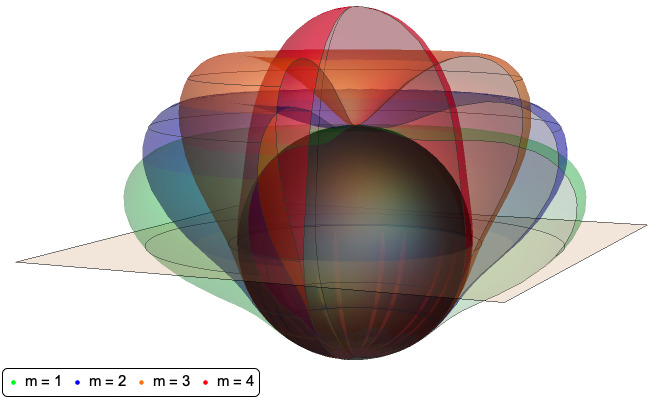
\includegraphics[width=9cm, height=5cm]{haldane eigenfunctions.jpg}
    \caption{\textit{Γραφική αναπαράσταση των ιδιοσυναρτήσεων για $s\subscr{0}=4$. Παρουσιάζονται τέσσερις από τις $2s\subscr{ο}+1$ ιδιοκαταστάσεις του τελεστή $L\subscr{z}$ με ιδιοτιμές $m\hbar$. (Πράσινο) $u\superscr{5}v\superscr{3}$ με $m=1$. (Μπλε) $u\superscr{6}v\superscr{2}$ με $m=2$. (Πορτοκαλί) $u\superscr{7}v$ με $m=3$. (Κόκκινο) $u\superscr{8}$ με $m=4$.}}
    \label{fig:haldane eigenfunctions s=4}
\end{figure}


%Για την περιγραφή σωματιδίου πάνω στη σφαίρα 
Προχωρούμε τώρα στη γραφική αναπαράσταση των πολυωνύμων Haldane \eqref{Haldane polynomial}. Καθορίζουμε αρχικά τις συνιστώσες $(a,b)$ του σπίνορα $\left| r\right>$ και τις εισάγουμε στην \eqref{Haldane polynomial}. 
%Οι συνιστώσες του $\left|r\right>$ είναι οι μιγαδικοί %συντελεστές των $2s\subscr{o}+1$ όρων στα πολυώνυμα Haldane και %προσδιορίζουν, όπως αναφέρθηκε προηγουμένως, το σημείο μέγιστης %πυκνότητας πιθανότητας. 
Για παράδειγμα, ας θεωρήσουμε τηω περίπτωση $s\subscr{0}=1$ και $\left|r\right>=(\cos\frac{\pi}{6}e\superscr{i\frac{\pi}{6}},\sin\frac{\pi}{6}e\superscr{-i\frac{\pi}{6}})$. Εφαρμόζοντας την \eqref{haldane wavefunction binomial}, η κυματοσυνάρτηση είναι
\begin{equation}
    \Psi\superscr{1}\subscr{r}\,=\,\sum\limits_{m=-1}^{1}\binom{2}{1+m}\left( \cos\frac{\pi}{6}\cos\frac{\theta}{2}e\superscr{i(\frac{\phi}{2}-\frac{\pi}{6})} \right)\superscr{1+m}\left( \sin\frac{\pi}{6}\sin\frac{\theta}{2} e\superscr{-i(\frac{\phi}{2}-\frac{\pi}{6})} \right)\superscr{1-m}
\end{equation}
Η αντίστοιχη πυκνότητα πιθανότητας φαίνεται στην εικόνα \ref{fig:haldane wavefunction s=1}. Είναι εμφανής η απουσία αζιμουθιακής συμμετρίας. Στη δεξιά εικόνα της \ref{fig:haldane wavefunction s=1}, απεικονίζεται μια τομή της γραφικής παράστασης, ώστε να διακρίνονται τα ακρότατα σημεία. Τα σημεία αυτά βρίσκονται αντιδιαμετρικά του $\vec{\Omega}\subscr{r}$. 
%, το διάνυσμα που συνδέεται με τον $\left|r\right>$ μέσω της %\eqref{position vector and spinor}. 
Στο σχήμα περιλαμβάνεται επίσης η μοναδιαία σφαίρα με κέντρο την αρχή των αξόνων.

\section{Πολυσωματιδιακές καταστάσεις φερμιονίων}
 Εάν αμελήσουμε τις αλληλεπιδράσεις μεταξύ των φορτισμένων σωματιδίων στις στάθμες Landau, η χαμιλτονιανή 
% αγνοώντας τις αλληλεπιδράσεις μεταξύ των φορτίων (integer hall %effect) 
 δίνεται από την έκφραση
\begin{equation*}
    H\,\approx\,\sum\subscr{i=1}\superscr{N}H\subscr{i}
\end{equation*}
όπου
\begin{figure}[t] 
    \centering
    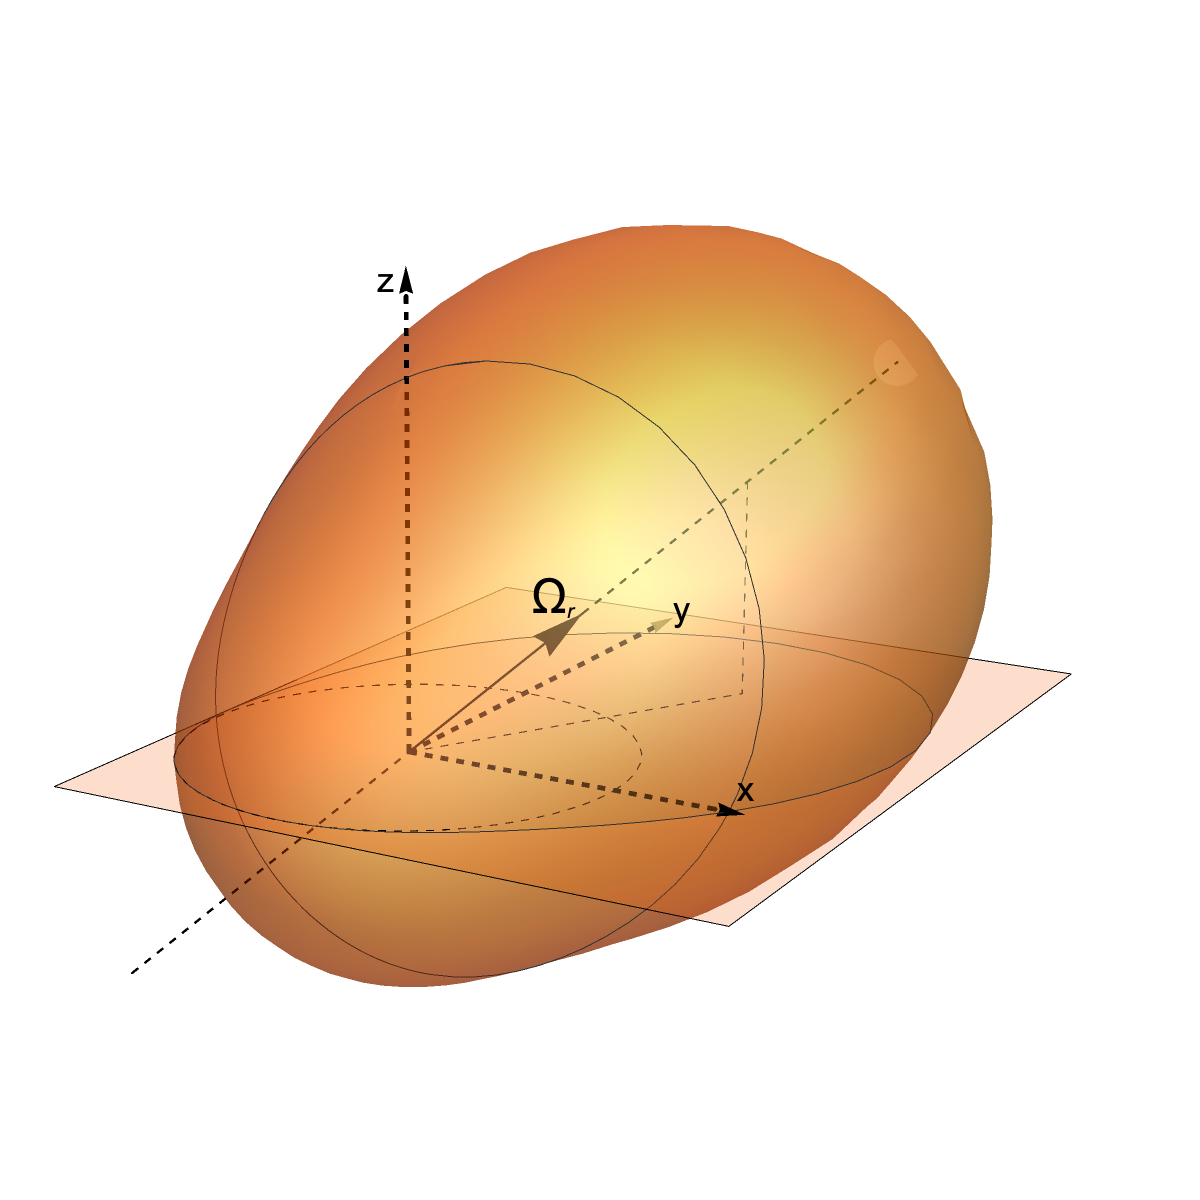
\includegraphics[width=7cm, height=8cm]{haldane wavefunction full.png}
    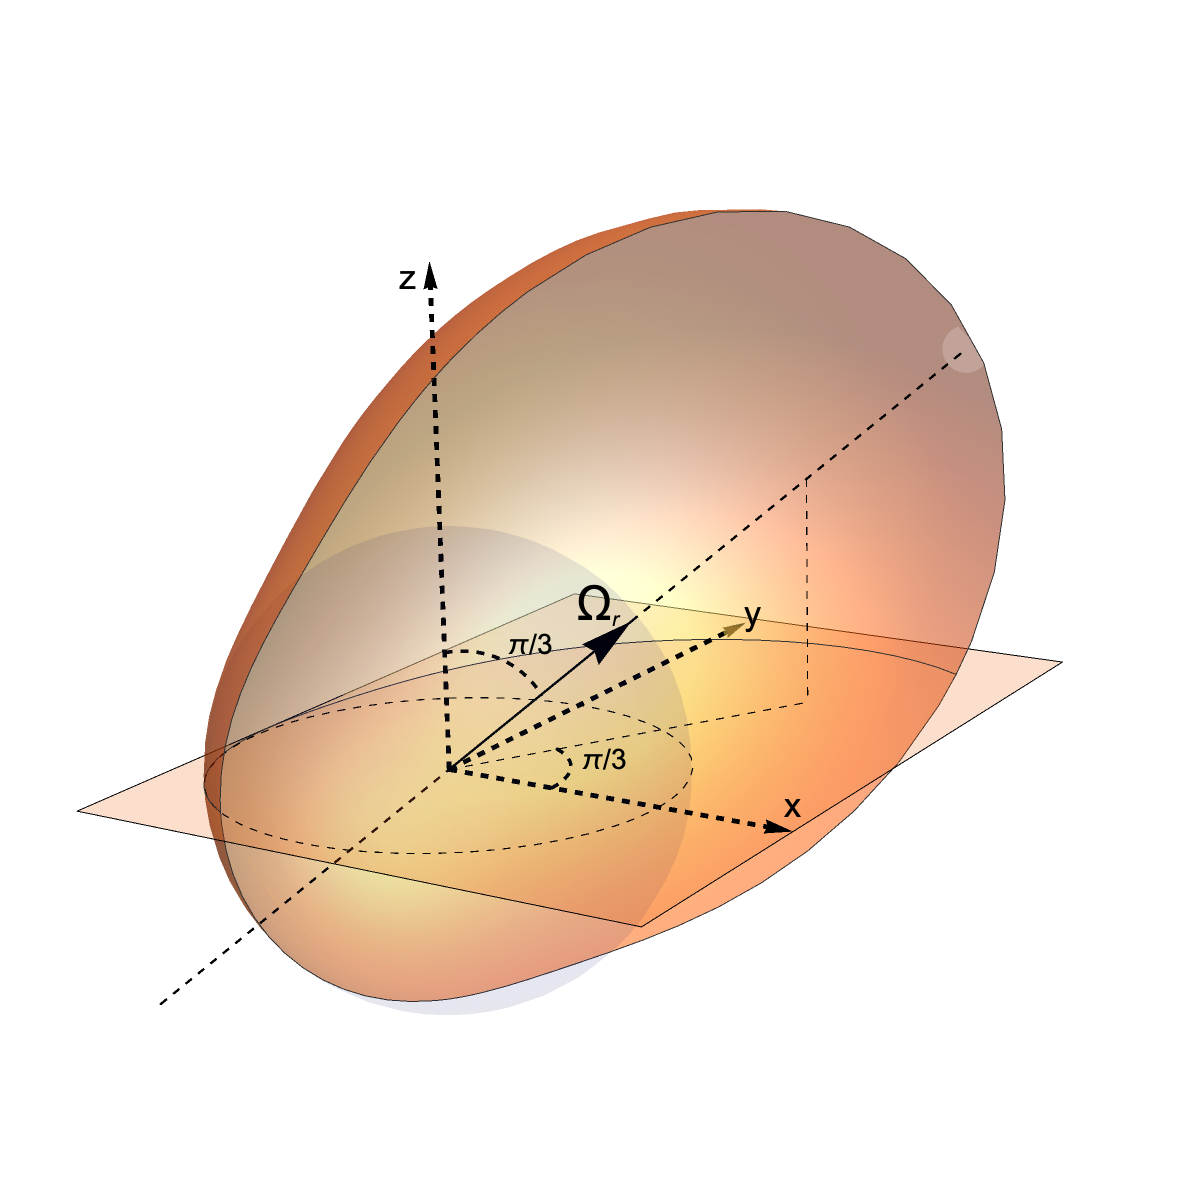
\includegraphics[width=7cm, height=8cm]{haldane wavefunction half.png}
    \caption{\textit{Γραφική αναπαράσταση της πυκνότητας πιθανότητας $|\Psi\superscr{1}\subscr{(a,b)}|^2$ για $s\subscr{0}=1$ και $\left|r\right>=(\cos\frac{\pi}{6}e\superscr{i\frac{\pi}{6}},\sin\frac{\pi}{6}e\superscr{-i\frac{\pi}{6}})$. Στο δεξιό σχήμα φαίνεται μια τομή της κυματοσυνάρτησης με το επίπεδο $\phi=\pi/3$, με μέγιστο στη θέση $\theta=\frac{\pi}{3},\phi=\frac{\pi}{3}$.}}
    \label{fig:haldane wavefunction s=1}
\end{figure}

%Η χαμιλτονιανή του συστήματος των Ν ασύζευτων σωματιδίων είναι %απλά το άθροισμα των μονοσωματιδιακών χαμιλτονιανών της μορφής \eqref{hamiltonian with magnetic monopole} 
\begin{equation*}
    H\subscr{i}\,=\,\frac{|\Lambda\subscr{i}|^2}{2m}\frac{eB}{\hbar s\subscr{0}}
\end{equation*}
η μονοσωματιδιακή χαμιλτονιανή.
%Η μηχανική στροφορμή $\Lambda\subscr{i}$ του σωματιδίου i %αντιστοιχεί στους γεννήτορες της άλγεβρας των περιστροφών %$L\subscr{i}$ 
(Ο δείκτης $i$ δηλώνει τα διάφορα σωματίδια).
%, όχι τις συνιστώσες) που ορίζονται όπως και στην \eqref{angular momentum algebra generators} και ικανοποιούν τις μεταθετικές σχέσεις \eqref{generator commutation relations}, ενώ μεταξύ δύο σωματιδίων i και j ισχύει ότι $[L\subscr{i},L\subscr{j}]=0$. 
Οι διάφορες μονοσωματιδιακές καταστάσεις καταλαμβάνονται σύμφωνα με την απαγορευτική αρχή του Pauli. Η ολική κυματοσυνάρτηση πρέπει να είναι αντισυμμετρική ως προς την εναλλαγή δύο οποιωνδήποτε φερμιονίων.
%Δεδομένου των προαναφερόμενων, είναι δυνατόν να φτιαχτεί %κατάσταση N σωματιδίων από το γινόμενο μονοσωματιδιακών %καταστάσεων. 
Όταν $N=2s\subscr{0}+1$, η χαμηλότερη στάθμη Landau είναι πλήρως κατειλημμένη. 
%LLL, αυτή δηλαδή των $N=2s\subscr{o}+1$ φερμιονίων, πρέπει να %γίνει η κατάληψη του LLL με τρόπο που σέβεται την απαγορευτική %αρχή του Pauli. Εφόσων έχουμε τόσα φερμιόνια όσος και ο %εκφυλισμός του LLL, 
Το κάθε φερμιόνιο καταλαμβάνει μια ανεξάρητη ορθογώνια μονοσωματιδιακή κατάσταση στη LLL, δες \eqref{basis of squared integrable functions on the sphere}.  
%ορθογώνια αυτής κάθε άλλου φερμιονίου. 
%Χρησιμοποιούμε τις ορθογώνιες μονοσωματιδιακές καταστάσεις %$\psi\subscr{s\subscr{o},m}$ της βάσης , με καλά ορισμένο κβαντικό %αριθμό m της z συνιστώσας της στροφορμής, $L\subscr{i,z}$. 
Προσδιορίζουμε την ολική κυματοσυνάρτηση $\Psi\subscr{N}$ 
%φτιάχνεται συνδυάζοντας τις $\psi\subscr{s\subscr{o},m}$ 
με χρήση της ορίζουσας Slater
\begin{equation}\label{slater determinant}
\Psi\subscr{N}\,=\,\left|\begin{array}{cccc}
    u\subscr{1}\superscr{2s\subscr{0}} & u\subscr{1}\superscr{2s\subscr{0}-1}v\subscr{1} &\dots & v\subscr{1}\superscr{2s\subscr{0}} \\
    u\subscr{2}\superscr{2s\subscr{0}} & \dots & \dots & v\subscr{2}\superscr{2s\subscr{0}} \\
    \vdots & \ddots & & \vdots\\
    u\subscr{N}\superscr{2s\subscr{0}} & u\subscr{N}\superscr{2s\subscr{0}-1}v\subscr{N} &\dots & v\subscr{N}\superscr{2s\subscr{0}}
\end{array}\right|
\end{equation}
%με τις σειρές του πίνακα να αντιστοιχούν σε ένα από τα %$2s\subscr{o}+1$ σωματίδια καθώς οι στήλες στις ιδιοκαταστάσεις %$\Psi\subscr{N}$. 
Η κυματοσυνάρτηση \eqref{slater determinant} γράφεται και στην ακόλουθη πιο απλή μορφή \cite{PhysRevLett.51.605}
\begin{equation}\label{haldane manyparticle wavefunction}
    \Psi\subscr{N}\,=\,\prod^{N}_{i<j}(u\subscr{i}v\subscr{j}-u\subscr{j}v\subscr{i})
\end{equation}
όπου $Ν$ ο εκφυλισμός της βασικής LLL (ή ο αριθμός των φερμιονίων)
\begin{equation}
    N=2s\subscr{0}+1
\end{equation}
Για συνοχή με τα προηγούμενα κεφάλαια 
%\cite{Maldacena_2021}, 
στα οποία η συνολική μαγνητική ροή συμβολίζεται με $Q$, θέτουμε $Q=2s_0$. Για μεγάλα $Q$, παίρνουμε λοιπόν
\begin{equation}
    N\approx Q\equiv 2s\subscr{0}
\end{equation}

\section{Εξίσωση διασποράς σχετικιστικών σωματιδίων}
%Στην περίπτωση κατάληψης του LLL από 
Για σχετικιστικά φερμιόνια με σπιν 1/2 και φορτίο $-e$, προσδιορίζουμε την εξίσωση διασποράς με βάση την εξίσωση Dirac. Σε επίπεδο χωροχρόνο, αυτή έχει τη μορφή
\begin{equation}\label{equation Dirac}
    \left( i \gamma\superscr{\mu}D\subscr{\mu} - m\right)\psi = 0
\end{equation}
όπου $\psi$ ο σπίνορας Dirac, $D\subscr{\mu}$ η συναλλοίωτη παράγωγος
\begin{equation}\label{covariant der}
\begin{split}
    &D\subscr{\mu}\equiv\partial\subscr{\mu}-ieA\subscr{\mu}\\
    &[D\subscr{\mu},D\subscr{\nu}]=-ieF\subscr{\mu\nu}
\end{split}
\end{equation}
και $F\subscr{\mu\nu}$ ο ηλεκτρομαγνητικός τανυστής του Maxwell
\begin{equation}
    F\subscr{\mu\nu}=\partial\subscr{\mu}A\subscr{\nu}-\partial\subscr{\nu}A\subscr{\mu}
\end{equation}
Δρούμε στα δύο μέλη της \eqref{equation Dirac} με τον μιγαδικό συζυγή του τελεστή Dirac και καταλήγουμε στην εξίσωση
\begin{equation}\label{dirac equation to klein gordon}
    (\gamma\superscr{\mu}\gamma\superscr{\nu}D\subscr{\mu}D\subscr{\nu}+m\superscr{2})\psi\,=\,0
\end{equation}
Με χρήση του μεταθέτη \eqref{gamma matrix commutator} και του αντιμεταθέτη \eqref{gamma matrix anticommutator} των πινάκων Dirac, η \eqref{dirac equation to klein gordon} παίρνει τη μορφή
\begin{equation}
    \frac{1}{2}(-4iS\superscr{\mu\nu}D\subscr{\mu}D\subscr{\nu}+2D\superscr{\mu}D\subscr{\mu})\psi+m\superscr{2}\psi\,=\,0
\end{equation}
Ο μεταθέτης \eqref{covariant der} εισάγει στην εξίσωση τον ηλεκτρομαγνητικό τανυστή
\begin{equation}
    \left[D\superscr{2} - iS\superscr{\mu\nu}(-ieF\subscr{\mu\nu}) +m\superscr{2}\right]\psi\,=\,0
\end{equation}
%της μορφής του $F\subscr{\mu\nu}$ 
Στην περίπτωση μη μηδενικού μαγνητικού πεδίου (δες \eqref{def of em tensor}) 
\begin{equation}
    \begin{split}
        &F\subscr{0i}=F\subscr{i0}=0\\
        &F\subscr{ij}=\epsilon\subscr{ijk}B\subscr{k}
    \end{split}
\end{equation}
όπου $B_k$ οι συνιστώσες του μαγνητικού πεδίου, και χρσιμοποιώντας την εκφραση του $S\superscr{\mu\nu}$ \cite{Peskin:1995ev}, η σχετικιστική εξίσωση ανάγεται στην
\begin{equation}\label{relativistic energy equation}
    \left[ D\superscr{2}\subscr{0}+(-iD\subscr{i})\superscr{2}-2e\Vec{B}\cdot\Vec{S}+m\superscr{2} \right]\psi\,=\,0
\end{equation}
Μετασχηματίζοντας στο χώρο των ορμών, ο πρώτος όρος δείνει το αρνητικό τετράγωνο της ενέργειας $-E\superscr{2}$ 
%όταν δράσει στην $\psi$ 
ενώ ο δεύτερος περιλαμβάνει τον τελεστή της μηχανικής ορμής, ο οποίος συνδέεται με την στροφορμή \eqref{mechanical momentum} ως εξής
\begin{equation}
    \Vec{\Pi}\superscr{2}\,=\,\frac{1}{r\superscr{2}}\left[ \Vec{\Lambda}\superscr{2}-i\Vec{r}\cdot\Vec{\Pi}+(\Vec{r}\cdot\Vec{\Pi})\superscr{2} \right]\,=\,\frac{\Lambda\superscr{2}}{r\superscr{2}}-\frac{1}{r\superscr{2}}\frac{\partial}{\partial r}r\superscr{2}\frac{\partial}{\partial r}
\end{equation}
Συμβολίζουμε την ακτινική ορμή με $p\subscr{3}$ 
\begin{equation}
     \Vec{\Pi}\superscr{2}\,=\,\frac{\Lambda\superscr{2}}{r\superscr{2}}+p\subscr{3}\superscr{2}
\end{equation}
Αντικαθιστούμε την ιδιοτιμή του τελεστή $\Lambda\superscr{2}$, δες \eqref{eigenvalues in LLL}, και βρίσκουμε 
\begin{equation}
    \frac{\Lambda\superscr{2}}{r\superscr{2}}=\frac{s\subscr{0}}{r\superscr{2}}=eB\equiv |F|
\end{equation}
Ο τρίτος όρος περιγράφει την αλληλεπίδραση του μαγνητικού πεδίου με το σπιν $\Vec{S}$
\begin{equation}
    2e\Vec{B}\cdot\Vec{S} = 2eBs \equiv 2|F|s
\end{equation}
%Στην $\ell$ αναπαράσταση της ομάδας Lorentz ο τελεστής S έχει %ιδιοτιμές $s=-\ell,\dots,\ell-1,\ell$. Συγκεκριμένα, για την %$\frac{1}{2}$ αναπαράσταση 
Για ένα φερμιόνιο οι ιδιοτιμές του σπιν είναι $\pm\frac{1}{2}$ (θέτουμε $\hbar=1$ ) από τις οποίες επιλέγεται η θετική για ισχυρά μαγνητικά πεδία. Ως αποτέλεσμα, να αλληλοαναιρούνται η ενεργειακή συνεισφορά εξαιτίας της αλληλεπίδρασης της τροχιακής στροφορμής με το μαγνητικό πεδίο και η συνεισφορά εξαιτίας της σύζευξης του σπιν με το μαγνητικό πεδίο. 
Τέλος, με βάση τα πιο πάν, η σχετικιστική εξίσωση διασποράς ανάγεται στην ακόλουθη
\begin{equation}\label{spinor energy magnetic field}
    E\superscr{2}(\text{spinor})-p\subscr{3}\superscr{2}\,=\,m\superscr{2}+|F|(1-2s)=m\superscr{2}+0,\qquad s=1/2
\end{equation}
\\

Για βαθμωτά πεδία (με σπιν $0$) και φορτίο $-e$, η αντίστοιχη εξίσωση είναι 
%ενέργεια δεν περιέχει τη σύζευξη μεταξύ spin και μαγνητικού %πεδίου και είναι
\begin{equation}\label{scalar energy}
     E\superscr{2}(\text{scalar})-p\subscr{3}\superscr{2}\,=\,m\superscr{2}+|F|,\qquad s=0
\end{equation}
Για φορτισμένα διανυσματικά πεδία με σπιν $1$ παίρνουμε \cite{Corben:1940zz}
%αναπαράστασης ισχύει η εξίσωση \eqref{spinor energy magnetic %field} της σπινορικής αναπαράστασης. Ο γυρομαγνητικός λόγος %$\gamma=2$ των σπιν 1 πεδίων φέρει τις ενεργειακές ιδιότητες %της αναπαράστασης, εντός μαγνητικού πεδίου, πολύ κοντά σε αυτές %των σπινόρων Dirac. Η σύζευξη των σπιν 1 πεδίων με %ηλεκτρομαγνητικό πεδίο και ο γυρομαγνητικός λόγος %παρουσιάζονται στο άρθρο  των Corben και Schwinger. H ενέργεια %για την ιδιοτιμή $s=1$ είναι 
\begin{equation}\label{vector boson energy magnetic field}
    E\superscr{2}(\text{vector})-p\subscr{3}\superscr{2}\,=\,m\superscr{2}+|F|(1-2s)=m\superscr{2}-|F|,\qquad s=1
\end{equation}
\\
%%%%%%%%%%%%%%%%%%%%%%%%%%%%%%%%%%%%%%%%%%%%%%%%%%%%%%%%%%%%%%%%%%%%%%%%%%%%%
%%%%%%%%%%%%%%%%%%%%%%%%%%%%%%%%%%%%%%%%%%%%%%%%%%%%%%%%%%%%%%%%%%%%%%%%%%%%%
Συνοψίζοντας τα παραπάνω, στη βασική στάθμη Landau $n=0$, οι εξισώσεις διασποράς για φορτισμένα βαθμωτά, φερμιονικά και διανυσματικά  πεδία είναι
\begin{equation}
    E\superscr{2}-p\subscr{3}\superscr{2}\,=\,\left\{\begin{array}{ll}
         m\superscr{2}+|F|, &s=0 \\
         m\superscr{2}+0, & s=1/2 \\
         m\superscr{2}-|F|, & s=1
    \end{array}\right.
\end{equation}

%%%%%%%%%%%%%%%%%%%%%%%%%%%%%%%%%%%%%%%%%%%%%%%%%%%%%%%%%%%%%%%%%%%%%%%%%%%%%
%%%%%%%%%%%%%%%%%%%%%%%%%%%%%%%%%%%%%%%%%%%%%%%%%%%%%%%%%%%%%%%%%%%%%%%%%%%%%
\begin{comment}
\section{Προχειρο}
και έτσι αναθέτουμε σε κάθε σωματίδιο μια ιδιοκατάσταση του 
Όταν το εκφυλισμένο χαμηλότερο επίπεδο Landau είναι πλήρως κατηλημένο από φερμιόνια η συνολική στροφορμή μηδενίζεται, $\Vec{L}=\sum_{i}^{\text{\scalebox{0.6}{$2s\subscr{o}+1$}}}\Vec{L\subscr{i}}=0$ - κάθε μία από τις $2s\subscr{o}+1$ ιδιοκαταστάσεις καταλαμβάνεται από ένα μόνο φερμιόνιο. Επομένως, δεν χρειάζεται να οριστεί διάνυσμα $\Omega\subscr{r}\text{\scalebox{0.7}{$(a,b)$}}$, όπως υπάρχει για παράδειγμα στην μονοσωματιδιακή κυματοσυνάρτηση \eqref{Haldane polynomial}, και έτσι η $\Psi\subscr{N}$ είναι ανεξάρτητη των (a,b). Σύμφωνα με την απαγορευτική αρχή του Pauli η $\Psi\subscr{N}$ πρέπει να είναι πλήρως αντισυμμετρική ως προς εναλλαγή δύο οποιωνδήποτε σωματιδίων. \\

Στο κείμενο του, ο Haldane, παρουσιάζει μεταξύ άλλων την αντισυμμετρική κυματοσυνάρτηση δύο φερμιονίων $\psi_{\text{\scalebox{0.8}{(a,b)}}}^{\text{\scalebox{0.8}{($s\subscr{o}$,j)}}}$. Στην παρουσία δύο σωματιδίων ο τελεστής της συνολικής στροφορμής είναι $\Vec{L}=\Vec{L}\subscr{1}+\Vec{L}\subscr{2}$. Ο τελεστής $L\superscr{2}$ έχει ιδιοτιμές j(j+1) όπου j παίρνει κβαντωμένες τιμές από 0 ($L\subscr{1}$, $L\subscr{2}$ αντιπαράλληλα) μέχρι 2$s\subscr{o}$ ($L\subscr{1}$, $L\subscr{2}$ παράλληλα) - στο LLL. Περιγράφει τις καταστάσεις με τα πολυώνυμα που ικανοποιούν την εξίσωση ιδιοτιμών
\begin{equation}
    \{\Omega\subscr{r}\cdot\Vec{L}\} \psi_{\text{\scalebox{0.8}{(a,b)}}}^{\text{\scalebox{0.8}{($s\subscr{o}$,j)}}}\,=\,\hbar j\,\psi_{\text{\scalebox{0.8}{(a,b)}}}^{\text{\scalebox{0.8}{($s\subscr{o}$,j)}}} \qquad 0\le\,j\,\le\,2s\subscr{o}
\end{equation}
Όπως και στην μονοσωματιδιακή περίπτωση έτσι και τώρα, η $\psi_{\text{\scalebox{0.8}{(a,b)}}}^{\text{\scalebox{0.8}{($s\subscr{o}$,j)}}}$ επικεντρώνεται γύρω από το σημείο με διάνυσμα $\Omega\subscr{r}(a,b)$ αντίστοιχο του σπίνορα (a,b)
\begin{equation}
    \psi_{\text{\scalebox{0.8}{(a,b)}}}^{\text{\scalebox{0.8}{($s\subscr{o}$,j)}}} \,=\, (u\subscr{1}v\subscr{2}-u\subscr{2}v\subscr{1})\superscr{2s\subscr{o}-j}\prod\limits_{i=1,2}(a\superscr{*}u\subscr{i}+b\superscr{*}v\subscr{i})\superscr{j}
\end{equation}
\end{comment}

%---------------------------------------------------------------------------
\chapter{Καθιερωμένο Πρότυπο}
Tο καθιερωμένο πρότυπο 
%της σωματιδιακής φυσικής τα σωματίδια ύλης και τα μποζόνια %βαθμίδας υπόκεινται στο μηχανισμό αυθόρμητης ρήξης της %συμμετρίας. Το πρότυπο 
βασίζεται στη θεωρία των Glashow, Weinberg και Salam, η οποία ενοποιεί τις ηλεκτρομγνητικές και τις ασθενείς αλληλεπιδράσεις %(ηλεκτρασθενής θεωρία) 
σε μια συμμετρική, μη-αβελιανή θεωρία βαθμίδας $SU(2)\subscr{L}\times U(1)\subscr{Y}$. Η ηλεκτρασθεής συμμετρία αυτή σπάζει αυθόρμητα (μηχανισμός Higgs) με σημαντικές φυσικές συνέπειες \cite{Peskin:1995ev}. Στο κεφάλαιο αυτό παρουσιάζουμε μερικές από τις συνέπειες αυτές, και τις επανεξετάζουμε στην περίπτωση ισχυρών μαγνητικών πεδίων υποβάθρου. Μία τέτοια κατάσταση εμφανίζεται στην εξωτερική περιοχή του ορίζοντα μιας μαγνητικά φορτισμένης μελανής οπής. 

\section{Αυθόρμητη ρήξη συμμετρίας}\label{spontaneous symmetry breaking}
Οι συμμετρίες ενός φυσικού μοντέλου είναι μετσχηματισμοί που αφήνουν αμετάβλητες παρατηρήσιμες φυσικές ποσότητες, όπως η ενέργεια. 
%των καταστάσεων του  αναφερόμαστε στην αμεταβλητότητα των %φυσικών ποσοτήτων ως προς μετασχηματισμούς των κβαντικών %καταστάσεων. 
Οι μετασχηματισμοί αναπαρίστανται ως εκθετικοί μοναδιακοί τελεστές $U=e\superscr{iT\superscr{i}\theta\superscr{i}}$ που δρουν στο χώρο Hilbert, $\mathcal{H}$, των κβαντικών καταστάσεων
\begin{equation}
    U:\mathcal{H}\rightarrow\mathcal{H}
\end{equation}
όπου $T^i$ οι ερμιτιανοί γεννήτορες των μετασχηματισμών (με τις απαραίτητες μεταθετικές ιδιότητες). Οι μοναδιακοί τελεστές δρουν γραμμικά στις κβαντικές καταστάσεις, οι οποίες 
%δρα σε συγκεκριμένους βαθμούς ελευθερίας των κβαντικών πεδίων %τα οποία, 
στη γενικότερη περίπτωση μεταβάλλονται
\begin{equation}\label{transformation of psi under the group of unitary operators}
    \left|\psi\right>\mapsto\left|\psi '\right>\equiv U\left|\psi\right> = e\superscr{iT\superscr{i}\theta\superscr{i}}\left|\psi\right> \qquad  \left|\psi\right>\ne \left|\psi'\right>
\end{equation}
Αντίθετα, εάν μια κατάσταση $ \left|\psi\right>$ παραμένει αναλλοίωτη, τότε είναι συμμετρική ως προς τους μετασχηματισμούς. Σε αυτή τη περίπτωση η $ \left|\psi\right>$ είναι ιδιοκατάσταση του τελεστή $U$ και καταστρέφεται από τους αντίστοιχους γεννήτορες
\begin{equation}\label{psi is symmetric under the unitary transformation of the group}
    \left|\psi\right>\mapsto U \left|\psi\right> = \left|\psi\right>, \qquad T\superscr{i} \left|\psi\right>=0
\end{equation}
%Η αλλοίωση όμως των κβαντικών καταστάσεων δεν μεταφέρεται κατ' %ανάγκη στη χαμιλτονιανή του φυσικού μοντέλου. 
\\

Οι μετασχηματισμοί λοιπόν που αφήνουν τη χαμιλτονιανή αναλλοίωτη αποτελούν συμμετρίες της θεωρίας. Οι αντίστοιχοι μοναδιακοί τελεστές και οι γεννήτορες τους μετατίθενται με τη χαμιλτονιανή
\begin{equation}\label{commutator with hamiltonian for a symmetry}
    [H,U]=[H,T\superscr{a}]=0
\end{equation}
%Είναι σημαντικό να σημειωθεί ότι η \eqref{commutator with %hamiltonian for a symmetry} ισχύει ανεξάρτητα του αν η %κατάσταση του συστήματος $\left|\psi\right>$ αλλοιώνεται από το %μετασχηματισμό \eqref{transformation of psi under the group of %unitary operators} ή όχι \eqref{psi is symmetric under the %unitary transformation of the group}. 
\\

Εκδηλώνονται σημαντικά φαινόμενα όταν η δράση των μετασχηματισμών συμμετρίας μεταβάλλουν τη βασική κατάσταση του συστήματος, ή την κατάσταση κενού σε ένα σύστημα κβαντικού πεδίου $\left|\,\Omega\right>$ 
%που ορίζεται ως η κατάσταση μηδενικής τετραορμής %$P\superscr{\mu}=(H,\vec{P})$ 
%\begin{equation}\label{vacuum state zero momentum}
%    P\superscr{\mu}\left|\,\Omega\right>=0\qquad\vec{P}\left|\,%\Omega\right>=0 
%\end{equation}
Η $\left|\,\Omega\subscr{i}\right>$ μετασχηματίζεται σε μια ορθογώνια κατάσταση $\left|\Omega\subscr{j}\right>$, σύμφωνα με την \eqref{transformation of psi under the group of unitary operators} 
\begin{equation}\label{transformation of vacuum state}
    \left|\,\Omega\subscr{i}\right> \mapsto \left|\Omega\subscr{j}\right> \equiv U\left|\,\Omega\subscr{i}\right>\ne \left|\,\Omega\subscr{i}\right> \qquad \left<\Omega\subscr{i}\,|\,\Omega\subscr{j}\right>=\de\subscr{ij}
\end{equation}
%γεγονός που την καθιστά μη συμμετρική ως προς τους %μετασχηματισμούς. 
Με χρήση του μεταθέτη \eqref{commutator with hamiltonian for a symmetry} είναι φανερό ότι η νέα κατάσταση $\left|\,\Omega'\right>$ είναι επίσης ιδιοκατάσταση της χαμιλτονιανής με την ίδια ιδιοτιμή 
\begin{equation}
    [H,U]\left|\,\Omega\right>=0\Rightarrow H(U\left|\,\Omega\right>)=UH\left|\,\Omega\right>=E\subscr{\Omega}U\left|\,\Omega\right>
\end{equation}
Οι εκφυλισμένες καταστάσεις έχουν την ίδια ενέργεια $E\subscr{\Omega}$ αλλά διαφορετικές αναμενόμενες τιμές για διάφορους άλλους τελεστές. Μια υπέρθεση όλων αυτών των καταστάσεων, όπως προβλέπεται στη μη σχετικιστική κβαντική μηχανική, σέβεται την συμμετρία και αίρει τον εκφυλισμό. 
Όπως δείχνουμε στη συνέχεια, η πραγματική βασική κατάσταση στην περίπτωση ενός κβαντομηχανικού μοντέλου δεν είναι κάποια από τις καταστάσεις που ελαχιστοποιούν τη δυναμική ενέργεια, αλλά μια συμμετρική υπέρθεση τους. Αντίθετα, στην κβαντική θεωρία πεδίων, οι βασικές καταστάσεις μπορεί να σπάζουν τη συμμτερία 
%να είναι μια από τις εκφυλισμένες καταστάσεις, η οποία όμως %είναι ευαίσθητη στους μετασχηματισμούς της ομάδας συμμετρίας 
σύμφωνα με την \eqref{transformation of vacuum state}. Όταν συμβαίνει αυτό θα λέμε ότι η συμμετρία σπάζει αυθόρμητα.

\subsection{Κβαντομηχανικό παράδειγμα}
Ως πρώτο παράδειγμα, ας θεωρήσουμε ένα μη σχετικιστικό κβαντικό σωματίδιο μάζας $m$ το οποίο κινείται σε μία διάσταση υπό την επίδραση δύναμης που απορρέει από το δυναμικό 
%και συνάρτηση πυκνότητας πιθανότητας $\psi(x)$ εντός του δυναμικού 
$V(x)= \frac{1}{2}m\omega\superscr{2}x\superscr{2}(x\superscr{2}-1)$. Η χαμιλτονιανή του συστήματος παραμένει αναλλοίωτη ως προς τη συμμτερία ομοτιμάς $x \to -x$, που είναι μια διακριτή $\mathbb{Z}\subscr{2}$ συμμετρία. Το δυναμικό έχει δύο ελάχιστα %σημεία ευσταθούς ισορροπίας 
για $x=a,-a$. Εκδηλώνει μέγιστο στη θέση $x=0$. Ένα κλασικό σωματίδιο με συνολική ενέργεια $E<V(0)$ είναι εξαναγκασμένο να εκτελεί ταλαντώσεις γύρω από ένα ελάχιστο, χωρίς να μπορεί να διέλθει του φράγματος δυναμικού. Αυτό όμως, δεν συμβαίνει στο κβαντικό επίπεδο εξαιτίας του φαινομένου της σήραγγας. Στο χώρο Hilbert, οι δύο εκφυλισμένες καταστάσεις είναι οι $\left|a\right>$ και $\left|-a\right>$ με την κάθε μια να επικεντρώνεται γύρω από την αντίστοιχη κλασική θέση ισορροπίας 
\begin{equation}
    \left<-a\right|\hat{x}\left|-a\right>=-a\qquad\left<a\right|\hat{x}\left|a\right>=a
\end{equation}
Οι δύο αυές καταστάσεις δεν περιγράφουν τη βασική κατάσταση του συστήματος, αφού το κβαντικό σωματίδιο μπορεί να διέλθει του φράγματος με μη μηδενική πιθανότητα, η οποία υπολογίζεται στην προσέγγιση WKB (π.χ. \cite{griffiths_qm})
\begin{equation}
    T=\exp\left[ -\frac{2}{\hbar}\int_{-a}^{a}dx\,[2m(V-E)]\superscr{1/2} \right]
\end{equation}
Η χαμιλτονιανή έχει τα εξής πινακοστοιχεία μεταξύ των δύο εκφυλισμένων καταστάσεων $\left|a\right>$ και $\left|-a\right>$: 
\begin{equation}
\begin{split}
    &\left<-a\right|\hat{H}\left|-a\right>=\left<a\right|\hat{H}\left|a\right>=\frac{1}{2}\hbar\omega\\
    &\left<-a\right|\hat{H}\left|a\right>=\left<a\right|\hat{H}\left|-a\right>=\frac{\hbar\omega}{2\pi}e\superscr{-m\omega a\superscr{2}/\hbar}
\end{split}
\end{equation}
Η βασική κατάσταση αποτελεί γραμμικό συνδυασμό των $\left|a\right>$ και $\left|-a\right>$. Πράγματι, ο εκφυλισμός αίρεται και η κατάσταση χαμηλότερης ενέργειας είναι ο συμμετρικός συνδυασμός $\left|S\right>$, με ενέργεια $E\subscr{\text{S}}$ που δίδεται από την έκφραση
\begin{equation}
    \left|S\right>=\frac{\left|a\right>+\left|-a\right>}{\sqrt{2}}\qquad E\subscr{S}=\frac{1}{2}\hbar\omega-\frac{\hbar\omega}{2\pi}e\superscr{-m\omega a\superscr{2}/\hbar}
\end{equation}
Η αναμενόμενη τιμή του τελεστή θέσης $\hat{x}$ στη βασική κατάσταση είναι επομένως αμετάβλητη ως κατοπτρικούς  μετασχηματισμούς ομοτιμίας, εξαιτίας της αναλλοιότητας της βασικής κατάστασης
\begin{equation}
    \left<S\right| \hat{x} \left|S\right>\,=\,0
\end{equation}

\subsection{Συνεχείς συμμετρίες και μποζόνια Goldstone}
Στη κβαντική θεωρία πεδίων, όταν σπάσουν αυθόρμητα συνεχείς καθολικές συμμετρίες 
%ομάδων Lie μπορούν να σπάσουν οδηγώντας σε ενδιαφέροντα %φαινόμενα. Η ρήξη καθολικών (global) συμμετριών συνοδεύεται από
εμφανίζονται άμαζα σωματίδια στο φάσμα, τα σωματίδια Goldstone, σύμφωνα με το θεώρημα Goldstone. Στην περίπτωση τοπικών  συμμετριών, οι καταστάσεις Goldstone συνδυάζονται με τα μποζόνια βαθμίδας για να δώσουν ένα σωματίδιο με σπιν $1$ και μη μηδενική μάζα \cite{Peskin:1995ev}.  
%που έχουν εισαχθεί για την αναλλοίωτη ως προς βαθμίδα %λειτουργία της θεωρίας. Είναι ενδιαφέρον ότι 
Tο αυθόρμητο
σπάσιμο συμμετρίας δεν εκδηλώνεται σε χωροχρόνους με δύο ή λιγότερες διαστάσεις λόγω των ισχυρών κβαντικών διακυμάνσεων των μποζονίων Goldstone. 
%σε αυτές τις διαστάσεις - απόδειξη του Sidney Coleman. 

\subsection{Κατάσταση κενού στην κβαντική θεωρία πεδίου}
Σε μια κβαντική θεωρία πεδίου, ενδέχεται οι καταστάσεις που ελαχιστοποιούν την ενέργεια να είναι εκφυλισμένες. Οι καταστάσεις αυτές μετασχηματίζονται η μια στην άλλη μέσω συμμετριών, όπως αναφέραμε προηγουμένως, και χαρακτηρίζονται από μη μηδενικές τιμές κάποιου πεδιακού τελεστή.
%Βάση όμως της αρχής cluster decomposition 
Στις τέσσερις διαστάσεις, είναι δυνατό το σύστημα να βρεθεί σε 
%περιοριστεί σε μόνο 
μία από τις εκφυλισμένες καταστάσεις αυτές, η οποία όμως δεν είναι αμετάβλητη, 
%καθιστώντας την κατάσταση κενού μη συμμετρική - 
οδηγώντας σε αυθόρμητο σπάσιμο της συμμετρίας. Αυτό μπορεί να δειχθεί εφαρμόζοντας την αρχή της ανάλυσης κατά κλάστερς \cite{weinberg_1996}.
Με βάση την αρχή αυτή τα αποτελέσματα πειραμάτων  
%αφορά την επιβολή της φυσικής προϋπόθεσης ότι, πειράματα 
σε περιοχές 
%απόμακρα σημεία 
του χώρου που απέχουν κατά πολύ μεγάλη απόσταση, δηλαδή για $\mathbf{x}\equiv \Vec{x}$, $\mathbf{\text{\textbf{y}}}\equiv \Vec{\text{y}}$, $|\mathbf{x}-\text{\textbf{y}}|\rightarrow\infty$, είναι ανεξάρτητα μεταξύ τους. Συνεπώς, στην πραγματική κατάσταση κενού, $\left|\text{VAC}\right>$, η αναμενόμενη τιμή γινομένου δύο πεδιακών τελεστών, σε δύο σημεία των περιοχών αυτών αντίστοιχα, παραγοντοποιείται σε γινόμενο των αναμενόμενων τιμών του κάθε τελεστή ξεχωριστά \cite{weinberg_1996}
\begin{equation}
    \lim\subscr{|\mathbf{x}-\text{\textbf{y}}|\rightarrow\infty}\left<\text{VAC}\right|A(\mathbf{x})B(\text{\textbf{y}})\left|\text{VAC}\right>=\left<\text{VAC}\right|A(\mathbf{x})\left|\text{VAC}\right>\left<\text{VAC}\right|B(\text{\textbf{y}})\left|\text{VAC}\right> \label{clusters}
\end{equation}
\\

Η αρχή δεν μπορεί να ικανοποιηθεί εάν
%μόνο αν οι φυσικές καταστάσεις είναι καθαρές (pure states) και %όχι 
η κατάσταση κενού $\left|\text{VAC}\right>$ αποτελεί υπέρθεση 
%(mixed states) 
των εκφυλισμένων καταστάσεων που ελαχιστοποιούν την ενέργεια. Αρχικά, μια κατάσταση κενού έχει μηδενική συνολική ορμή 
%\eqref{vacuum state zero momentum} 
και είναι επομένως αναλλοίωτη ως προς χωρικές μετατοπίσεις ή αλλιώς στη δράση του τελεστή μετατοπίσεων 
\begin{equation}\label{vacuum spatial transl invariance}
    \hat{T}(\mathbf{x})\left|\Omega\right>=\left|\Omega\right> \qquad \hat{T}(x)\equiv e\superscr{-i\mathbf{x}\cdot\mathbf{P}}
\end{equation}
Ένας πεδιακός τελεστής $A$ στη θέση $\mathbf{x}$ μπορεί να γραφτεί συναρτήσει του τελεστή στην αρχή των αξόνων $\mathbf{0}$ και του τελεστή μεταφοράς ως εξής
\begin{equation}\label{operator spatial translation}
    A(\mathbf{x})=\hat{T}(\mathbf{x})A(0)\hat{T}\superscr{-1}(\mathbf{x})
\end{equation}
Επομένως τα πινακοστοιχεία του μεταξύ των εκφυλισμένων καταστάσεων κενού είναι ανεξάρτητα της θέσης 
\begin{equation}
    \left<\Omega\subscr{i}\right|A(\mathbf{x})\left|\Omega\subscr{k}\right>=\left<\Omega\subscr{i}\right|A(0)\left|\Omega\subscr{k}\right>
\end{equation}
\\

Ας θεωρήσουμε ότι το φάσμα των εκφυλισμένων καταστάσεων κενού είναι διακριτό \cite{weinberg_1996}. Τότε ο μοναδιαίος πίνακας (στον χώρο των μονοσωματιδιακών καταστάσεων) δίδεται από την εξής σχέση πληρότητας 
%μπορεί να γραφτεί ως η πρόσθεση του αθροίσματος των %εκφυλισμένων καταστάσεων κενού μηδενικής ορμής με την %ολοκλήρωση του συνεχούς φάσματος των καταστάσεων καλά ορισμένης %ορμής $\mathbf{p}\equiv \Vec{p}$
(ο δείκτης $m$ συμβολίζει άλλος βαθμούς ελευθερίας) 
%που συμβολίζονται με m
\begin{equation}
    \mathbf{1}=\sum\subscr{\Omega}\left|\Omega\right>\left<\Omega\right|\,+\,\int \sum\subscr{m}d\superscr{3}\mathbf{p}\left|\mathbf{p},m\right>\left<\mathbf{p},m\right|
\end{equation}
Παρεμβάλλοντας τη σχέση πληρότητας στη συνάρτηση συσχέτισης 
%τον ταυτοτικό τελεστή στο ενδιάμεσο του ισόχρονου γινομένου 
δύο ερμιτιανών τελεστών παίρνουμε
\begin{equation}
    \left<\Omega\subscr{i}\right|A(\mathbf{x})\mathbf{1}B(\mathbf{\text{\textbf{y}}})\left|\Omega\subscr{k}\right>=\sum\subscr{\Omega} \left<\Omega\subscr{i}\right|A(\mathbf{x})\left|\Omega\right>\left<\Omega\right|B(\mathbf{\text{\textbf{y}}})\left|\Omega\subscr{k}\right>\,+\,\int d\superscr{3}\mathbf{p}\left<\Omega\subscr{i}\right|A(\mathbf{x})\left|\mathbf{p}\right>\left<\mathbf{p}\right|B(\mathbf{\text{\textbf{y}}})\left|\Omega\subscr{k}\right>
\end{equation}
Με χρήση των \eqref{operator spatial translation} και \eqref{vacuum spatial transl invariance} η προηγούμενη εξίσωση ανάγεται στην ακόλουθη
\begin{equation}
    \sum\subscr{\Omega} \left<\Omega\subscr{i}\right|A(0)\left|\Omega\right>\left<\Omega\right|B(0)\left|\Omega\subscr{k}\right>\,+\,\int d\superscr{3}\mathbf{p}\left<\Omega\subscr{i}\right|A(0)\left|\mathbf{p}\right>\left< \mathbf{p}\right|B(0)\left|\Omega\subscr{k}\right>e\superscr{i\mathbf{p}\cdot(\mathbf{x}-\mathbf{y})}
\end{equation}
Το ολοκλήρωμα στον χώρο των ορμών μηδενίζεται στο όριο $|\mathbf{x}-\text{\textbf{y}}|\rightarrow\infty$, εξαιτίας της έντονα διακυμενόμενης φάσης, 
%δεδομένου ότι οι συναρτήσεις που συνοδεύουν το μιγαδικό %εκθετικό είναι διαφορίσιμες (smooth) σε όλο το χωρίο της %ολοκλήρωσης. Ο μηδενισμός υποστηρίζεται από το 
με βάση το θεώρημα Riemann-Lebesgue. Το αποτέλεσμα ισχύει και εάν μεταθέσουμε τους δύο τελεστές. Επομένως παίρνουμε
\begin{equation}\label{vacuum limit with identity operator}
\begin{split}
    &\lim\subscr{|\mathbf{x}-\text{\textbf{y}}|\rightarrow\infty}\left<\Omega\subscr{i}\right|A(\mathbf{x})B(\text{\textbf{y}})\left|\Omega\subscr{k}\right>\,=\,\sum\subscr{n} \left<\Omega\subscr{i}\right|A(0)\left|\Omega\subscr{n}\right>\left<\Omega\subscr{n}\right|B(0)\left|\Omega\subscr{k}\right>\\
    &\lim\subscr{|\mathbf{x}-\text{\textbf{y}}|\rightarrow\infty}\left<\Omega\subscr{i}\right|B(\text{\textbf{y}})A(\mathbf{x})\left|\Omega\subscr{k}\right>\,=\,\sum\subscr{n} \left<\Omega\subscr{i}\right|B(0)\left|\Omega\subscr{n}\right>\left<\Omega\subscr{n}\right|A(0)\left|\Omega\subscr{k}\right>
\end{split}
\end{equation}
Επιπρόσθετα, με βάση την αρχή της αιτιότητας, ο μεταθέτης δύο χωροειδώς διαχωρισμένων τοπικών τελεστών 
μηδενίζεται. Επομένως, για ισόχρονα σημεία $[A(\mathbf{x}),B(\text{\textbf{y}})]=0$. 
%για χωροειδής $(x-\text{y})\superscr{2}>0$ και επομένως για %ισόχρονα $\mathbf{x}\ne\text{\textbf{y}}$ διαστήματα. 
Εφόσον οι τελεστές είναι ερμιτιανοί και μετατίθενται, πρέπει να διαγονοποιούνται ταυτόχρονα στη βάση $\left|\Omega\right>$. Επομένως τα πινακοστοιχεία στα δεξιά μέλη της \eqref{vacuum limit with identity operator} ικανοποιούν τη σχέση
\begin{equation}
    \left<\Omega\subscr{i}\right|\mathcal{O}(0)\left|\Omega\subscr{k}\right>=\de\subscr{ik}a\subscr{k}
\end{equation}
με αποτέλεσμα να ισχύει η ανάλυση κατά κλάστερς, \eqref{clusters}, σε μια από τις εκφυλισμένες καταστάσεις $|{\Omega}\rangle$. 
Αντίθετα, εάν η πραγματική κατάσταση του κενού αποτελεί  υπέρθεση των εκφυλισμένων καταστάσεων $|{\Omega}\rangle$, παίρνουμε
\begin{equation}
    \left<\text{VAC}\right|A(\mathbf{x})B(\mathbf{\text{\textbf{y}}})\left|\text{VAC}\right>=\sum\subscr{n} \left<\text{VAC}\right|A(0)\left|\Omega\subscr{n}\right>\left<\Omega\subscr{n}\right|B(0)\left|\text{VAC}\right>
\end{equation}
Το μη τετριμμένο άθροισμα φανερώνει ότι είναι αδύνατον να ικανοποιηθεί η αρχή της ανάλυσης σε κλάστερς. 
%cluster decomposition. 
%Αντιθέτως, εάν το πραγματικό κενό είναι μια μόνο από τις %εκφυλισμένες καταστάσεις τότε ικανοποιείται. 
Έτσι, σε ένα χώρο με άπειρη διαστατικότητα, το σύστημα μπορεί να βρίσκεται σε μια από τις εκφυλισμένες καταστάσεις $|{\Omega}\rangle$, και συνεπώς σπάζει αυθόρμητα η συμμετρία.


\section{Τοπική θεωρία βαθμίδας}\label{section local gauge theory}
%Οι ηλεκτρομαγνητικές και ασθενής αλληλεπιδράσεις περιγράφονται %στο καθιερωμένο πρότυπο ως εκφάνσεις μιας αλληλεπίδρασης. 
Οι ηλεκτρασθενείς αλληλεπιδράσεις περιγράφονται από μια θεωρία Yang-Mills με συμμετρία βαθμίδος $SU(2)\subscr{L}\times U(1)\subscr{Y}$. Ο δείχτης $L$ στην ομάδα $SU(2)$ δηλώνει τη χειραλικότητα της θεωρίας, αφού μόνο τα αριστερόστροφα φερμιόνια αλληλεπιδρούν με τα μποζόνια βαθμίδος $SU(2)$. \\
%που φαίνεται να ξεχωρίζει μεταξύ αριστερόστροφων και %δεξιόστροφων σωματιδίων. 

Έχοντας επιλέξει την ομάδα συμμετρίας, η Λαγκραντζιανή πρέπει να είναι αναλλοίωτη κάτω από τους αντίστοιχους τοπικούς μετασχηματισμούς βαθμίδας. Τέτοιοι μετασχηματισμοί έχουν την μορφή
\begin{equation}\label{electroweak transformation}
    \phi\rightarrow e\superscr{i\alpha\superscr{i}\frac{\sigma\superscr{i}}{2}}e\superscr{i\beta Y}\phi\qquad Y\equiv \y\sigma\superscr{0}
\end{equation}
όταν το πεδίο $\phi$ βρίσκεται στην βασική αναπαράσταση της $SU(2)$, όπου $\frac{\sigma\superscr{i}}{2}$, $Y$ οι γεννήτορες των ομάδων $SU(2)$ και $U(1)$, αντίστοιχα, που δίδονται συναρτήσει πινάκων Pauli. Οι τέσσερις συναρτήσεις $\alpha\superscr{i}(x)$ και $\beta(x)$ είναι συνεχείς και διαφορίσιμες συναρτήσεις του χωροχρόνου. Η  αναλλοιώτητα των κινητικών όρων επιτυγχάνεται αναβαθμίζοντας τη μερική παράγωγο στη συναλλοίωτη παράγωγο 
\begin{equation}
    \partial\subscr{\mu}\,\rightarrow\,D\subscr{\mu}\equiv\partial\subscr{\mu}-igW\superscr{i}\subscr{\mu}\frac{\sigma\superscr{i}}{2}-ig\subscr{\y}B\subscr{\mu}Y
\end{equation}
όπου τα μποζονικά πεδία βαθμίδας $W\superscr{i}\subscr{\mu}$, $B\subscr{\mu}$ συνοδεύουν τους γεννήτορες των ομάδων $SU(2)$ και $U(1)$ αντίστοιχα. 
%και εγγυούνται τον επιθυμητό μετασχηματισμό της συναλλοίωτης %παραγώγου. 
Τα πεδία βαθμίδας υπόκεινται στους ακόλουθους μετασχηματισμούς
\begin{equation}
\begin{split}
    W\superscr{i}\subscr{\mu}&\rightarrow W\superscr{i}\subscr{\mu}+\frac{1}{g}\partial\subscr{\mu}\alpha\superscr{i}-\epsilon\superscr{ijk}\alpha\superscr{j}W\superscr{k}\subscr{\mu}\\
    B\subscr{\mu}&\rightarrow B\subscr{\mu}+\frac{1}{g\subscr{\y}}\partial\subscr{\mu}\beta
\end{split}
\end{equation}
Όροι μάζας για τα πεδία βαθμίδας απαγορεύονται λόγω μη αναλλοιώτητας, ενώ επιτρέπονται κινητικοί όροι φτιαγμένοι από τους τανυστές $G\superscr{i}\subscr{\mu\nu}$ και $B\subscr{\mu\nu}$ 
\begin{equation}\label{tensors for electroweak gauge fields}
    \begin{split}
        &G\superscr{i}\subscr{\mu\nu}\,=\,\partial\subscr{\mu}W\superscr{i}\subscr{\nu}-\partial\subscr{\nu}W\superscr{i}\subscr{\mu}+g\epsilon\superscr{ijk}W\superscr{j}\subscr{\mu}W\superscr{k}\subscr{\nu}\\
        &B\subscr{\mu\nu}\,=\,\partial\subscr{\mu}B\subscr{\nu}-\partial\subscr{\nu}B\subscr{\mu}
    \end{split}
\end{equation}
Οι κινητικοί όροι των μποζονίων βαθμίδας στη Λαγκραντζιανή, ώστε αυτή να μένει αμετάβλητη κάτω από τοπικούς μετασχηματισμούς βαθμίδας, είναι
\begin{equation}\label{kinetic terms of electroweak gauge fields}
    \mathcal{L}\subscr{K}\,=\,-\frac{1}{4}G\subscr{\mu\nu}\superscr{i}G\superscr{i\,\mu\nu}-\frac{1}{4}B\subscr{\mu\nu}B\superscr{\mu\nu}
\end{equation}
Η Λαγκραντζιανή του ηλεκτρασθενούς μοντέλου στην απουσία φερμιονίων δίδεται από το άθροισμα της \eqref{kinetic terms of electroweak gauge fields} και της Λαγκραντζιανής του πεδίου Higgs, \eqref{scalar boson lagragian}, η οποία παρουσιάζεται στην επόμενη ενότητα
\begin{equation}\label{electroweak lagragian, sum of two lagragians, gauge field lagr and phi lagr}
    \mathcal{L}\,=\,\mathcal{L}\subscr{K}+\mathcal{L}\subscr{\phi}
\end{equation}
\section{Εισαγωγή πεδίου Higgs}
\begin{figure}[t] 
    \centering
    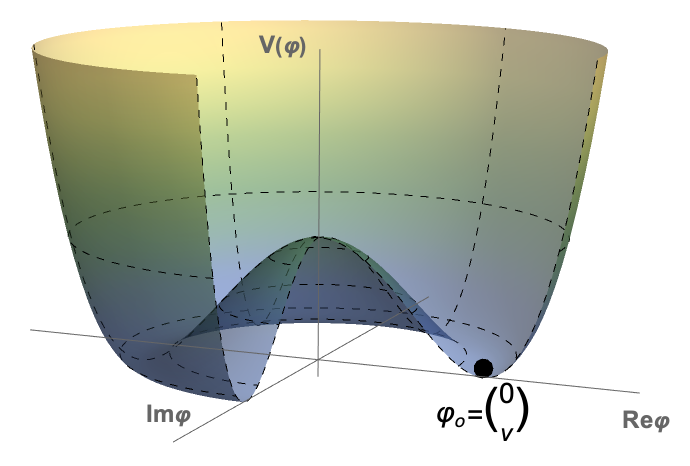
\includegraphics[width=7cm, height=5cm]{mexhat.png}
    \caption{\textit{Η συνάρτηση δυναμικού του μιδαδικού πεδίου $\phi$.}}
    \label{fig:mexhat}
\end{figure}
Για παραχθούν όροι μάζας για τα μποζόνια βαθμίδας 
%με μάζα. Αυτή η ανεπάρκεια επικρατεί γενικά στις τοπικές %θεωρίες βαθμίδας και θεραπεύεται με την 
εισάγουμε ένα βαθμωτό πεδίο, $\phi$, στη βασική αναπαράσταση της ομάδας $SU(2)$ - το πεδίο Higgs. Οι τέσσερις βαθμοί ελευθερίας (β.ε.) του πεδίου $\phi$ 
\begin{equation}\label{scalar SU doublet}
    \phi\,=\,\left(\begin{array}{c} \phi\superscr{+}\\ \phi\superscr{0} \end{array}\right), \qquad\phi\superscr{0},\phi\superscr{+}\in\mathbb{C}
\end{equation}
μετασχηματίζονται σύμφωνα με την \eqref{electroweak transformation}.
Η συνάρτηση δυναμικού του πεδίου πρέπει να ικανοποιεί τις ιδιότητες της επανακανονικοποίησης και να σέβεται τις συμμετρίες ως προς τους $SU(2)\subscr{L}\times U(1)\subscr{Y}$ μετασχηματισμούς. Η πιο γενική Λαγκραντζιανή 
%συνάρτηση βαθμωτού πεδίου που ικανοποιεί τα προαναφερόμενα 
είναι
\begin{equation}\label{scalar boson lagragian}
    \mathcal{L}\subscr{\phi}\,=\,|D\subscr{\mu}\phi|\superscr{2}-V(\phi)\,=\,|D\subscr{\mu}\phi|\superscr{2}+\mu\superscr{2}\phi\superscr{\dagger}\phi - \lambda(\phi\superscr{\dagger}\phi)\superscr{2}
\end{equation}
Όταν οι δύο παραμέτροι $\mu\superscr{2},\lambda\in\mathbb{R}$ ειναι θετικές, το δυναμικό ελαχιστοποιείται από ένα σύνολο εκφυλισμένων καταστάσεων για τις οποίες ισχύει
\begin{equation}
\begin{split}
    &|\phi|\superscr{2}=v\superscr{2},\quad v\in \mathbb{R}\\
    &\min V(\phi\superscr{\dagger}\phi)=V(v\superscr{2})
\end{split}
\end{equation}
\\

Εάν $\left|\Omega\right>$ είναι μια κατάσταση κενού, στην οποία η αναμενόμενη τιμή του πεδιακού τελεστή $\phi$ είναι μη μηδενική, $\left<\Omega\right|{\phi}\left|\Omega\right>\ne 0$, 
τότε αυτή πρέπει να μετασχηματίζεται κάτω από τη δράση της μοναδιακού τελεστή $U(g)$ (όπου $g\in SU(2)\subscr{L}\times U(1)\subscr{Y}$), στην ορθοκανονική κατάσταση $\left|\Omega'\right>\equiv U\left|\Omega\right>$, με την ίδια ενέργεια αλλά διαφορετική αναμενόμενη τιμή για τον πεδιακό τελεστή $\phi$: 
\begin{equation}\label{vacuum exp value symmetry group action}
    \left<\Omega'\right|{\phi}\left|\Omega'\right> = e\superscr{i\alpha\superscr{i}\frac{\sigma\superscr{i}}{2}}e\superscr{i\beta Y}\left<\Omega\right|{\phi}\left|\Omega\right>
\end{equation}
Από τη συζήτηση της ενότητας \ref{spontaneous symmetry breaking} αναμένουμε ότι η πραγματική κατάσταση κενού θα είναι 
%συμμετρική αλλά θα επιλεγεί 
μια από τις εκφυλισμένες καταστάσεις $\left|\Omega\right>$, με μη μηδενική αναμενόμενη τιμή $\left<\phi\right>$. 
%Έχοντας περιοριστεί σε μια συγκεκριμένη κατάσταση, το πεδίο %απαγορεύεται να "μεταβεί" σε κάποια άλλη από το εκφυλισμένο %σύνολο. Μια τέτοια μετάβαση αντιστοιχεί στη δράση της ομάδας %συμμετρίας ή κάποιου υποσυνόλου. Επομένως, η απαγόρευση %μετάβασης
Ως αποτέλεσμα οι β.ε. της διπλέτας που περιγράφουν το κενό δεσμεύονται και κάποια από τα σωματίδια βαθμίδας αποκτούν μάζα. %Οποιαδίποτε διπλέτα γράφεται ως η δράση στοιχείων της ομάδας %συμμετρίας στη γενική διπλέτα \eqref{scalar SU doublet} και το %αντίστροφο. 
Μια γενική διπλέτα παράγεται από μια $SU(2)$ περιστροφή συγκεκριμένης διπλέτας με $\phi\superscr{+}=0$ και $\phi\superscr{0}\in\mathbb{C}$
\begin{equation}\label{scalar doublet with zero comp and su2 tran}
    \phi\,=\,e\superscr{i\xi\superscr{i}\frac{\sigma\superscr{i}}{2}}\left(\begin{array}{c} 0\\ \phi\superscr{0} \end{array}\right)
\end{equation}
Η 
%δράση με την αντίστροφη 
περιστροφή αφήνει την $\mathcal{L}\subscr{\phi}$ αναλλοίωτη και καθιστά μια γενική διπλέτα \eqref{scalar SU doublet} ισοδύναμη %(όσον αφορά την $\mathcal{L}\subscr{\phi}$) 
με την 
%απλούστερη 
\begin{equation}\label{scalar doublet with zero comp}
    \Bar{\phi}\subscr{0}\,=\,\left(\begin{array}{c} 0\\ \phi\superscr{0} \end{array}\right)
\end{equation}
Με βάση τη 
%χρήση της 
διπλέτα \eqref{scalar doublet with zero comp}, "δεσμεύονται" δύο από τους τέσσερις β.ε. του πεδίου Higgs \cite{itzykson2012quantum}. 
%Αυτή η περιστροφή είναι, η ίδια, ένας μετασχηματισμός βαθμίδας %και ακολουθείται από απαραίτητους μετασχηματισμούς σε δυναμικά %βαθμίδας και άλλα πεδία που συνοψίζονται στο . 
Για να βρούμε το ελάχιστο του δυναμικού, βρίσκεται αντικαθιστούμε για $\Bar{\phi}\subscr{0}$ στο δυναμικό, $V(\phi\superscr{\dagger}\phi)$, και ελαχιστοποιούμε
%με διερεύνηση των ακρότατων 
ως προς $x\equiv|\phi\superscr{o}|\superscr{2}$. Έτσι, βρίσκουμε ένα σύνολο ελαχίστων για διάφορες τιμές του πραγματικού και φανταστικού μέρους της συνιστώσας $\phi\superscr{0}$ με μέτρο
\begin{equation}           v\superscr{2}\equiv\phi\superscr{0\,*}\phi\superscr{0}=(\operatorname{Re}\phi\superscr{0})\superscr{2}+(\operatorname{Im}\phi\superscr{0})\superscr{2}=\frac{\mu\superscr{2}}{2\lambda}
\end{equation}
Το σύνολο των τιμών αυτών αντιστοιχεί στην κυκλική βάση του δυναμικού της γραφικής παράστασης \ref{fig:mexhat}.\\

%Επαναλαμβάνοντας τα προηγούμενα βήματα, 
Η \eqref{scalar doublet with zero comp} παράγεται από έναν $SU(2)\times U(1)$ μετασχηματισμό μιας διπλέτας με μια μόνο πραγματική συνιστώσα
\begin{equation}\label{real scalar doublet and u1 tran}
    \Bar{\phi}\subscr{0}=e\superscr{i\alpha (x)}\left(\begin{array}{c} 0\\ v \end{array}\right),\qquad v=\sqrt{\frac{\mu\superscr{2}}{2\lambda}}
\end{equation}
%Είναι αρκετό να χρησιμοποιηθεί η διπλέτα στα δεξιά της %\eqref{real scalar doublet and u1 tran} εκτελώντας τον %αντίστροφο μετασχηματισμό και 
Δευσμεύοντας λοιπόν ακόμη έναν από τους τέσσερεις β.ε. του πεδίου Higgs, αρκεί να χρησιμοποιήσουμε τη διπλέτα
\begin{equation}\label{real scalar doublet}
     \phi\subscr{0}=\left(\begin{array}{c} 0\\ v \end{array}\right)
\end{equation}
Οι τέσσερις συνολικά γεννήτορες της ομάδας $SU(2)\subscr{L}\times U(1)\subscr{Y}$ 
%(τρεις της SU(2) και ένας από U(1)) 
αντιστοιχούν με τους τέσσερις β.ε. του πεδίου Higgs \eqref{scalar SU doublet}. Η \eqref{real scalar doublet} αντιστοιχεί στη μαύρη κουκίδα της εικόνας \ref{fig:mexhat}. Τρεις ανεξάρτητες συμμετρίες σπάζουν, αλλά παραμένει μια που αφήνει την  \eqref{real scalar doublet} αναλλοίωτη. Συνδυάζοντας το γεννήτορα $\frac{\sigma\superscr{3}}{2}$ της $SU(2)$ με τον γεννήτορα $Y$ της $U(1)$, παίρνουμε
\begin{equation}
\left(\begin{array}{cc}
     1 & 0 \\
     0 & 0
\end{array}\right) \phi\subscr{0} = 0
\end{equation}
έχοντας θέσει το υπερφορτίο του $\phi$ ίσο με $\y=\frac{1}{2}$, έτσι ώστε $Y=\frac{\sigma\superscr{0}}{2}$. Έτσι, βρίσκουμε το υποσύνολο των μετασχηματισμών που δεν σπάζουν και αφήνουν την  $\phi\subscr{0}$ αναλλοίωτη:
\begin{equation}
    \phi\subscr{0}\rightarrow e\superscr{i f(x)\,{Q}}\,\phi\subscr{0}=\phi\subscr{0}
\end{equation}
Οι πιο πάνω μετασχηματισμοί σχηματίζουν μια ομάδα $U(1)$ με γεννήτορα τον $Q$
\begin{equation}\label{electric charge quantum number}
    Q\equiv\frac{\sigma\superscr{3}}{2}+Y
\end{equation}
%- αργότερα θα ταυτιστεί με τον κβαντικό αριθμό ηλεκτρικού %φορτίου. Εν τέλη, η κατάσταση του κενού έχει καταλήξει με μια %μόνο (από τις τέσσερεις) πραγματική παράμετρο και παράλληλα ένα %υποσύνολο μετασχηματισμών που την αφήνει αμετάβλητη. 
Οι τρεις β.ε. του πεδίου Higgs που έχουν "δευσμευτεί" απορροφούνται από τα τρία μποζόντια των σπασμένων συμμετριών βαθμίδος παράγοντας τρία διανυσματικά πεδία με μη μηδενική μάζα. %μεταδότες των ασθενών ρευμάτων που αποκτούν μάζα. 

\section{Μάζες μποζονίων βαθμίδας}
Ακολουθούμε την ανάλυση 
%μαθηματική παραγωγή των μαζών 
του Peskin \cite{Peskin:1995ev} και εξετάζουμε τον κινητικό όρο του μποζονικού πεδίου Higgs. Η συναλλοίωτη παράγωγος είναι 
%που εμπεριέχονται στις συναλλοίωτες μερικές παραγώγους $|D\subscr{\mu}\phi|\superscr{2}$ 
\begin{equation}\label{covariant derivative electroweak theory}
    D\subscr{\mu}\equiv\partial\subscr{\mu}-igW\superscr{i}\subscr{\mu}\tau\superscr{i}-ig\subscr{\text{y}}B\subscr{\mu}Y\qquad\tau\superscr{i}\equiv\frac{\sigma\superscr{i}}{2}
\end{equation}
Δρώντας στην κατάσταση $\phi\subscr{0}$, η οποία είναι ομογενής, οι μερικές παράγωγοι μηδενίζονται και έτσι παίρνουμε
\begin{equation}
\begin{split}
    |D\subscr{\mu}\phi\subscr{0}|\superscr{2}\,&=\,\phi\subscr{0}\superscr{\dagger}\,\,(gW\superscr{i}\subscr{\mu}\frac{\sigma\superscr{i}}{2}+g\subscr{\y}B\subscr{\mu}Y)\superscr{2}\,\,\phi\subscr{0}\\
    &=\,\phi\subscr{0}\superscr{\dagger}\,\,(\frac{g}{4}W\superscr{2}\mathbf{1}+gg\subscr{\y}W\superscr{3}\sigma\superscr{3}Y+(g\subscr{\y}BY)\superscr{2})\,\,\phi\subscr{0}
\end{split}
\end{equation}
Με βάση τη \eqref{real scalar doublet} και το υπερφορτίο του $\phi$, βρίσκουμε
\begin{equation}
    |D\subscr{\mu}\phi\subscr{0}|\superscr{2}\,=\,\frac{1}{4}v\superscr{2}g\superscr{2}W\superscr{2}-\frac{1}{2}v\superscr{2}gg\subscr{\y}W\superscr{3}B+\frac{1}{4}(vg\subscr{\y})\superscr{2}B\superscr{2}
\end{equation}
Καταλήγουμε σε τρεις όρους με μάζας, 
οι οποίοι 
%τρεις όροι 
γράφονται στην 
%πιο οικεία 
μορφή γινομένου πινάκων 
%που θυμίζει όρο μάζας
\begin{equation}
    |D\subscr{\mu}\phi\subscr{0}|\superscr{2}\,=\,\frac{1}{2}\,(m\superscr{2})\superscr{ab}\Gamma\superscr{a}\subscr{\mu}\Gamma\superscr{b\,\mu}
\end{equation}
όπου
%με τους δείχτες a,b να προσδιορίζουν τα στοιχεία της τετραπλέτας των μποζονικών πεδίων 
\begin{equation}\label{A quadraplet}
    \Gamma\subscr{\mu}\equiv (W\superscr{1}\subscr{\mu}, W\superscr{2}\subscr{\mu}, W\superscr{3}\subscr{\mu}, B\subscr{\mu})
\end{equation}
και $m\superscr{2}$ ο πίνακας μάζας
\begin{equation}
    m\superscr{2}\equiv\frac{v\superscr{2}}{2}\left(\begin{array}{cccc}
        g^2 & 0 & 0 & 0 \\
        0 & g^2 & 0 & 0 \\
        0 & 0 & g^2 & -gg\subscr{\y} \\
        0 & 0 & -gg\subscr{\y} & g\subscr{\y}^2
    \end{array}\right)
 \end{equation}
Ο πίνακας μάζας όμως δεν είναι διαγώνιος για την εξαγωγή των μαζών των φυσικών σωματιδίων. Διαγωνοποιούμε τον πίνακα μάζας $m\subscr{D}\superscr{2}$ με τον ακόλουθο μετασχηματισμό ομοιότητας 
%του $m\superscr{2}$
\begin{equation}\label{diagonal mass matrix}
    m\superscr{2}\subscr{D}\,=\,E\superscr{-1}\,m\superscr{2}\,E\,=\,\frac{v\superscr{2}}{2}\,\cdot\,\text{diag}\left(g\superscr{2}\,,\,g\superscr{2}\,,\,(g\superscr{2}+g\subscr{\y}\superscr{2})\,,\,0\right)
\end{equation}
όπου 
%οι στήλες του πίνακα Ε είναι τα ιδιοδιανύσματα του %$m\superscr{2}$ (εκφρασμένα ως γραμμικοί συνδυασμοί των %στοιχείων της τετραπλέτας \eqref{A quadraplet})
\begin{equation}
    E \,=\, \left( \begin{array}{cccc}
         1 & 0 & 0 & 0 \\
         0 & 1 & 0 & 0 \\
         0 & 0 & \frac{g}{\sqrt{g\superscr{2}+g\subscr{\y}\superscr{2}}} & \frac{g\subscr{\y}}{\sqrt{g\superscr{2}+g\subscr{\y}\superscr{2}}}\\
         0 & 0 & \frac{-g\subscr{\y}}{\sqrt{g\superscr{2}+g\subscr{\y}\superscr{2}}} & \frac{g}{\sqrt{g\superscr{2}+g\subscr{\y}\superscr{2}}}
    \end{array} \right)
\end{equation}
Ο μετασχηματισμός ομοιότητας οδηγεί στην νέα βάση μποζονίων βαθμίδας, ως εξής 
%που αποτελείται από τα στοιχεία της τετραπλέτας $W'$
\begin{equation}
    W\subscr{\mu}'\equiv (W\superscr{1}\subscr{\mu},W\superscr{2}\subscr{\mu},Z\superscr{0}\subscr{\mu},A\subscr{\mu}) = (E\superscr{-1})\superscr{ab}\Gamma\superscr{b}\subscr{\mu}
\end{equation}
Τα πεδία $W\superscr{3}$ και $B$ της αρχικής βάσης περιστρέφονται 
%εντός του δυσδιάστατου αυθαίρετου χώρου που ορίζουν, 
στα πεδία $Z\superscr{0}$ και $A$. Το πρώτο, με μάζα $\frac{v}{\sqrt{2}}\sqrt{g\superscr{2}+g\subscr{\y}\superscr{2}}$, αντιστοιχεί στο συνδυασμό
\begin{equation}\label{Z boson}
    Z\subscr{\mu}\superscr{0}\,:=\,\frac{gW\subscr{\mu}\superscr{3}-g\subscr{\y}B\subscr{\mu}}{\sqrt{g\superscr{2}+g\subscr{\y}\superscr{2}}}
\end{equation}
και είναι συζευγμένο με τα ουδέτερα ρεύματα των ασθενών αλληλεπιδράσεων.
Το δεύτερο, με μηδενική μάζα, είναι ο φορέας των ηλεκτρομαγνητικών αλληλεπιδράσεων, το φωτόνιο
\begin{equation}\label{A boson}
    A\subscr{\mu}\,:=\,\frac{g\subscr{\y}W\superscr{3}\subscr{\mu}+gB\subscr{\mu}}{\sqrt{g\superscr{2}+g\subscr{\y}\superscr{2}}}
\end{equation}
Τα πεδία $W\superscr{1}$ και $W\superscr{2}$ αποκτούν μάζα $\frac{vg}{\sqrt{2}}$, και αποτελούν τους ηλεκτρικά φορτισμένους φορείς των ασθενών αλληλεπιδράσεων
\begin{equation}
    W\superscr{\pm}\subscr{\mu}\equiv \frac{1}{\sqrt{2}}(W\superscr{1}\subscr{\mu}\mp iW\superscr{2}\subscr{\mu})
\end{equation}
Συνδέονται με τους αντίστοιχους συνδυασμούς των γεννητόρων $\tau\superscr{1}$ και $\tau\superscr{2}$
\begin{equation}
    \tau\superscr{\pm}\equiv \tau\superscr{1}\pm i\tau\superscr{2}
\end{equation}
Ο ορθογώνιος πίνακας $\Bar{E}\superscr{-1}$ που παράγει την  περιστροφή
\begin{equation}
\left(\begin{array}{c}Z\superscr{0}\\A\end{array}\right)=\underbrace{\frac{1}{\sqrt{g\superscr{2}+g\subscr{\y}\superscr{2}}}\left(\begin{array}{cc}
    g & -g\subscr{\y} \\
    g\subscr{\y} & g
\end{array}\right)}_{\Bar{E}\superscr{-1}}\left(\begin{array}{c}W\superscr{3}\\B\end{array}\right)
\end{equation}
μπορεί να εκφραστεί ως πίνακας περιστροφής στο επίπεδο, συναρτήσει της γωνίας $\theta\subscr{w}$ 
\begin{equation}
\Bar{E}\superscr{-1}\equiv\left(\begin{array}{cc}
    \cos\theta\subscr{w} & -\sin\theta\subscr{w} \\
    \sin\theta\subscr{w} & \cos\theta\subscr{w}
\end{array}\right)
\end{equation}
η οποία ονομάζεται η ασθενής γωνία πρόσμιξης.
Ο λόγος των σταθερών σύζευξης ισούται με την εφαπτομένη της γωνίας πρόσμιξης 
\begin{equation}
    \tan\theta\subscr{w}\,\equiv\,\frac{g\subscr{\y}}{g}
\end{equation}
Επομένως μπορούμε να υπολογίσουμε τη γωνία $\theta\subscr{w}$ με βάση τον λόγο των μαζών των σωματιδίων $W$ και $Z$ 
\begin{equation}
    \theta\subscr{w}\,=\,\cos\superscr{-1}\frac{m\subscr{W}}{m\subscr{Z}}\sim 28^{\circ}
\end{equation}
\\

Τέλος, στη νέα βάση, η συναλλοίωτη παράγωγος \eqref{covariant derivative electroweak theory} γράφεται ως
%συναρτήσει των ιδιοπεδίων \eqref{Z boson} και \eqref{A boson}
\begin{equation}\label{covariant derivative with eigenstates}
    D\subscr{\mu}\equiv \partial\subscr{\mu}-i\frac{g}{\sqrt{2}}(W\superscr{+}\subscr{\mu}\tau\superscr{+}+W\superscr{-}\subscr{\mu}\tau\superscr{-})-i\frac{g}{\cos\theta\subscr{w}}Z\superscr{0}\subscr{\mu}(\tau\superscr{3}-\sin\superscr{2}\theta\subscr{w}Q)-ieA\subscr{\mu}Q
\end{equation}
Έχοντας ταυτίσει το πεδίο $A\subscr{\mu}$ με το φωτόνιο, βρίσκουμε τη σταθερά σύζευξη του με φορτισμένα πεδία
\begin{equation}
    e \equiv \frac{gg\subscr{\y}}{\sqrt{g\superscr{2}+g\subscr{\y}\superscr{2}}}=g\sin\theta\subscr{w}
\end{equation}
Το ηλεκτρικό φορτίο ταυτίζεται με την ιδιοτιμή του γεννήτορα $Q$: 
%με τον κβαντικό αριθμό ηλεκτρικού φορτίου
\begin{equation}
    Q=\tau\superscr{3}+Y
\end{equation}
%Η μορφή του Q είναι όπως και στην \eqref{electric charge %quantum number} με τη διαφορά ότι το υπερφορτίο %$Y=\y\sigma\superscr{o}$ καθορίζεται ανάλογα με την SU(2) %αναπαράσταση και το ηλεκτρικό φορτίο του πεδίου στο οποίο δρα ο %τελεστής \eqref{covariant derivative with eigenstates}. 
Η λαγκραντζιανή της ηλεκτρασθενούς θεωρίας, στη βαθμίδα όπου το Higgs δίδεται από την πραγματική διπλέτα που παρουσιάσαμε πιο πάνω, και αγνοώντας τους φερμιονικούς όρους, δίδεται συναρτήσει των φυσικών πεδίων $A\subscr{\mu},Z\subscr{\mu}$, $W\subscr{\mu}\equiv W\subscr{\mu}\superscr{+}$, $W^{\dagger}\subscr{\mu}\equiv W\subscr{\mu}\superscr{-}$
\begin{equation}\label{electroweak lagragian in terms of physical fields}
\begin{split}
    \mathcal{L}=& -\frac{1}{2}|\overline{D}\subscr{\mu}W\subscr{\nu}-\overline{D}\subscr{\nu}W\subscr{\mu}|\superscr{2}\,\,-\,\,\frac{1}{4}F\subscr{\mu\nu}\superscr{2}\,\,-\,\,\frac{1}{4}Z\subscr{\mu\nu}\superscr{2}\,\,+\,\,(\partial\subscr{\mu}\phi)\superscr{2}\\
    & +\frac{1}{2}g\superscr{2}\phi\superscr{2}|W\subscr{\mu}|\superscr{2}\,\,+\,\,\frac{1}{2}\frac{g\superscr{2}\phi\superscr{2}}{2\cos\superscr{2}\theta\subscr{w}}Z\subscr{\mu}\superscr{2}\\
    & -ig\left(\sin\theta\subscr{w}F\subscr{\mu\nu}+\cos\theta\subscr{w}Z\subscr{\mu\nu}\right)W\superscr{\dagger\,\mu}W\superscr{\nu}\\
    & +\frac{1}{2}g\superscr{2}\left( (W\subscr{\mu}\superscr{\dagger}W\subscr{\nu})\superscr{2}-(W\superscr{\dagger}\subscr{\mu}W\superscr{\mu})\superscr{2} \right)\\
    &-\lambda(\phi\superscr{2}-v\superscr{2})\superscr{2}
\end{split}
\end{equation}
Η συναλλοίωτη παράγωγος των μποζονίων W είναι η ακόλουθη
\begin{equation*}
    \overline{D}\subscr{\mu}\equiv\partial\subscr{\mu}-ig(\cos\theta\subscr{w}Z\subscr{\mu}+\sin\theta\subscr{w}A\subscr{\mu})
\end{equation*}
Η αρχική συμμετρία είναι σπασμένη στην $U(1)$ συμμετρία του ηλεκτρομαγνητισμού.

\section{Φερμιόνια στο καθιερωμένο Πρότυπο}
Η αυθόρμητη ρήξη της συμμετρίας από το πεδίο Higgs επιτρέπει την εισαγωγή φερμιονικών όρων μάζας. 
%ενώ ήταν αρχικά αδύνατο να συμπεριληφθούν ρητά στην %Λαγκρατζιανή. 
Σε αντίθεση με το καθιερωμένο πρότυπο, η θεωρία Dirac για ένα σχετικιστικό φερμιονικό πεδίο επιδέχεται άμεσα όρους μάζας, καθώς η απαίτηση για αναλλοιώτητα κατά Lorentz ικανοποιείται εύκολα
\begin{equation}\label{Dirac lagragian}
    \mathcal{L}\subscr{D}=\Bar{\psi}(i\slashed{\partial}-m)\psi
\end{equation}
Οι σπίνορες $\psi$ του Dirac γράφονται συναρτήσει ενός αριστερόστροφου $\psi\subscr{L}$ και δεξιόστροφου $\psi\subscr{R}$ σπίνορα ως εξής
\begin{equation}
    \psi\,=\, \left( \frac{1-\gamma\superscr{5}}{2} \right)\psi+\left( \frac{1+\gamma\superscr{5}}{2} \right)\psi \equiv \psi\subscr{L}+\psi\subscr{R}
\end{equation}
Αντικαθιστώντας στην \eqref{Dirac lagragian} και χρησιμοποιώντας τις ταυτότητες $\{\gamma\superscr{5},\gamma\superscr{0}\}=0$, $(\gamma\superscr{5})\superscr{2}=1$, $(\gamma\superscr{5})\superscr{\dagger}=\gamma\superscr{5}$, βρίσκουμε ότι οι όροι μάζας με δύο $\psi\subscr{L}$ ή δύο $\psi\subscr{R}$ μηδενίζονται:
\begin{equation}
    m\Bar{\psi}\subscr{L}\psi\subscr{L}=\Bar{\psi}\left( \frac{1+\gamma\superscr{5}}{2} \right)\left( \frac{1-\gamma\superscr{5}}{2}\psi \right) = 0
\end{equation}
%ενώ συμβαίνει το αντίθετο με τους κινητικούς όρους. 
Η αναλλοιότητα ως προς μετασχηματισμούς βαθμίδας στο καθιερωμένο πρότυπο απαγορεύει όρους μάζας με έναν αριστερόστροφο και έναν δεξιόστροφο σπίνορα
\begin{equation}\label{dirac mass terms}
    m\bar{\psi}\subscr{L}\psi\subscr{R}
\end{equation}
\subsection{Χειραλικότητα}
Εξαιτίας της χειραλικότητας των ασθενών αλληλεπιδράσεων 
%είναι η αιτία της διαφοράς μεταξύ των μετασχηματισμών 
μετασχηματίζονται διαφορετικά οι δεξιόστροφοι και οι αριστερόστροφοι σπίνορες ως προς μετασχηματισμούς βαθμίδας. %πεδίων και κατ΄επέκταση έχει καταληκτικές συνέπειες για τους %όρους μάζας. 
Τα δεξιόστροφα φερμιόνια, $\psi\subscr{R}$, δεν αλληλεπιδρούν ασθενώς. Επομένως μετασχηματίζονται σύμφωνα με την τετριμμένη μοναδιαία αναπαράσταση (singlet) της $SU(2)$. Το ηλεκτρικό τους φορτίο ισούται με το υπερφορτίο. Ως προς μετασχηματισμούς 
%της ομάδας 
βαθμίδας, μετασχηματίζονται με μια μιγαδική φάση, ανάλογα με το υπερφορτίο τους 
%που οφείλεται στο U(1) κομμάτι
\begin{equation}
    \psi\subscr{R}\rightarrow e\superscr{i\beta\y}\psi\subscr{R}
\end{equation}
\\

Τα αριστερόστροφα φερμιόνια αλληλεπιδρούν ασθενώς %αλληλεπιδράσεις 
και συνεπώς οι μετασχηματισμοί βαθμίδας εμπλέκουν την ομάδα $SU(2)$.
%παίρνουν διαφορετική μορφή. 
Οι λεπτονικές διεργασίες ασθενών αλληλεπιδράσεων σέβονται αυστηρά την ταξινόμηση σε τρεις λεπτονικές οικογένειες: $e$, $\mu$ και $\tau$ και διατηρούν τους τρεις 
%αντίστοιχους 
λεπτονικούς αριθμούς.
Για παράδειγμα, οι διασπάσεις $\mu\rightarrow e\Bar{\nu}\subscr{e}\nu\subscr{\mu}$ και $e\superscr{-}\rightarrow\nu\subscr{e}W\superscr{-}$ παρατηρούνται πειραματικά, όχι όμως οι διασπάσεις $W\superscr{-}\rightarrow e\nu\subscr{\mu}$, $\mu\rightarrow e\nu\subscr{e}\Bar{\nu}\subscr{\mu}$, $\mu\rightarrow e\gamma$. Οι ασθενείς αλληλεπιδράσεις 
%φαίνεται μόνο να περιστρέφουν 
εμπλέκουν κάθε αριστερόστροφο λεπτόνιο και το αντίστοιχο αριστερόστροφο νετρίνο. 
%και το αντίστροφο.
Έτσι, τα λεπτόνια μετασχηματίζονται στη βασική αναπαράσταση της $SU(2)$ σχηματίζοντας τις διπλέτες
\begin{equation}
    \ell\subscr{L}\superscr{i}\equiv\left(\begin{array}{c} \nu\subscr{i} \\ i \end{array}\right)\subscr{L},\qquad i=e,\mu,\tau
\end{equation}
%με τα στοιχεία κάθε διπλέτας να έχουν τον ίδιο λεπτονικό αριθμό %οικογένειας. 
Παρομοίως τα quarks ταξινομούνται σε τρεις οικογένειες ως ακολούθως
\begin{equation}
    q\subscr{L}\equiv \left(\begin{array}{c} u \\ d \end{array}\right)\subscr{L},\,\left(\begin{array}{c} c \\ s \end{array}\right)\subscr{L},\,\left(\begin{array}{c} t \\ b \end{array}\right)\subscr{L} 
\end{equation}
Σε αντίθεση με την διατήρηση των λεπτονικών αριθμών, 
%στα quarks δεν ισχύει το ανάλογο. Οι 
υπάρχουν ασθενείς διεργασίες 
%έχουν δείξει πειραματικά να 
που εμπλέκουν quarks από διαφορετικές οικογένειες, όπως για παράδειγμα, η διάσπαση $s\rightarrow uW\superscr{-}$ \cite{Griffiths:111880}. \\
%Λεπτομέρειες για αυτή τη συμπεριφορά των ασθενών αλλ. στο %κεφάλαιο 10 του . 

Τα αριστερόστροφα φερμιόνια λοιπόν $\psi\subscr{L}\equiv\ell\superscr{i}\subscr{L},\,q\subscr{i,L}$ μετασχηματίζονται ως ακολούθως
\begin{equation}
    \psi\subscr{L}\rightarrow e\superscr{i\alpha\superscr{i}\frac{\sigma\superscr{i}}{2}}e\superscr{i\beta Y}\psi\subscr{L}
\end{equation}
Επομένως οι όροι μάζς \eqref{dirac mass terms}
%, αν και αναλλοίωτη κατά Lorentz, 
δεν είναι αναλλοίωτοι ως προς τους μετασχηματισμούς βαθμίδας και έτσι δεν μπορούν να εμφανιστούν στην $\mathcal{L}$. \\

Το υπερφορτίο κάθε διπλέτας μπορεί να προσδιοριστεί με βάση 
%τον κβαντικό αριθμό 
το ηλεκτρικό φορτίο Q \eqref{electric charge quantum number}. Για παράδειγμα, οι συνιστώσες της διπλέτας $\ell\superscr{e}\subscr{L}$ έχουν ηλεκτρικά φορτία 0 και -1, αντίστοιχα και έτσι το υπερφορτίο που αντιστοιχεί στη διπλέτα ισούται με $\y=-\frac{1}{2}$. Οι συνιστώσες της διπλέτας των quarkς $q\subscr{u,L}$ έχουν ηλεκτρικά φορτία $\frac{2}{3}$ και $-\frac{1}{3}$ αντίστοιχα, και επομένως το υπερφορτίο ισούται με $\y=+\frac{1}{6}$.


\subsection{Η πλήρης θεωρία \texorpdfstring{$SU(3)\,\times\,SU(2)\,\times\,U(1)$}{TEXT}}
Το καθιερωμένο πρότυπο περιλαμβάνει επίσης την περιγραφή των ισχυρών αλληλεπιδράσεων των quarks. Η περιγραφή βασίζεται σε μια μη αβελιανή θεωρία βαθμίδας με ομάδα την $SU(3)$. Οι ομάδα αυτή έχει οκτώ γεννήτορες και επομένως υπάρχουν οκτώ φορείς για την ισχυρή δύναμη, τα γκλουόνια, που είναι άμαζα σωματίδια με σπιν 1. 
%κατασκευάζει τη μη αβελιανή θεωρία βαθμίδας με τα απορρέοντα %οκτώ (όσα και οι γεννήτορες) άμαζα σπιν-1 μποζόνια στην συζυγή %αναπαράσταση (adjoint representation) να είναι οι μεταδότες των %ισχυρών δυνάμεων - gluons. 
Τα quarks έχουν την ιδιότητα του χρώματος 
%στο πλαίσιο των ισχυρών δυνάμεων διεκδικούν φορτίο, τον %κβαντικό αριθμό χρώματος (color) 
με τρείς τιμές, κόκκινο (r), πράσινο (g) και μπλε (b) και έτσι μετασχηματίζονται με βάση τη θεμελιώδη αναπαράσταση της $SU(3)$ με διαστατικότητα 3. 
%Τα gluons αλληλεπιδρούν με τα quarks αλλάζοντας το χρωματικό %τους φορτίο. 
Σε αυτό το σημείο, 
Τα φερμιόνια της πρώτης οικογένειας μπορούν να ταξινομηθούν με βάση τις $U(1)$, $SU(2)$ και $SU(3)$ αναπαραστάσεις τους - δες πίνακα \ref{tab:table with particles and su3, su2 representations}. 

\begin{table}
    \centering
    \begin{tabular}{|m{0.25cm}|m{4.5cm}|m{2cm}|m{2cm}|m{1.9cm}|m{1.4cm}|}
    \cline{2-6}
    \multicolumn{1}{m{0.25cm}|}{} & \centering \textbf{(3,2,1/6)} & \centering \textbf{(3,1,2/3)} & \centering \textbf{(3,1,-1/3)} & \centering \textbf{(1,2,-1/2)} & \textbf{(1,1,-1)} \\
    \hline
     \rotatebox{90}{SU(2)} & \[ \left(\left(\begin{array}{c}
         u^r \\ \\ d^r
    \end{array}\right)_L,\left(\begin{array}{c}
        u^g \\ \\ d^g
    \end{array}\right)_L, \left(\begin{array}{c}
         u^b \\ \\ d^b 
    \end{array}\right)_L\right)\] & \center{$(u^r,u^g,u^b)\subscr{R}$} & \center{$(d^r,d^g,d^b)\subscr{R}$} & \[\left(\begin{array}{c}
         \nu \\ \\ e
    \end{array}\right)_L\] & $\quad\, e_R$ \\
    \hline
    \multicolumn{1}{c}{} & \multicolumn{5}{|c|}{\textbf{SU(3)}} \\
    \cline{2-6}
    \end{tabular}
    \caption{\textit{Οι αναπαραστάσεις των φερμιονίων ως προς τις ομάδες συμμετρίας του καθιερωμένου προτύπου.}}
    %SU(2) - διαστατικότητας d=2 (διπλέτες) για τα %αριστερόστροφα (L) και d=1 (singlets) για τα δεξιόστροφα %(R). Ταυτόχρονα, οι αναπαραστάσεις ως προς SU(3) - d=3 %(τριπλέτες) για τα quarks και διαστατικότητας 1 (singlets) %για τα λεπτόνια. Το υπερφορτίο Y της U(1) βαθμίδας είναι το %τρίτο στοιχείο στην αρχή κάθε στοίλης, π.χ. 1/6 για τα L %quarks.
    \label{tab:table with particles and su3, su2 representations}
\end{table}

\subsection{Φερμιονικοί όροι μάζας}\label{section mass for fermions}
%Ανίκανοι να χρησιμοποιήσουμε όρους μάζας καταφεύγουμε στην 
Αξιοποιούμε το μηχανισμό Higgs με βάση τον οποίο τα μποζόνια βαθμίδος αποκτούν μάζα. Εισάγουμε στους όρους \eqref{dirac mass terms} το πεδίο $\phi$ με υπερφορτίο $y=1/2$
\begin{equation}
    \Bar{\psi}\subscr{L}\cdot\phi\psi\subscr{R} \,+\, \text{h.c.}
\end{equation}
επιτυγχάνοντας έτσι την αναλλοιότητα ως προς όπλους τους μετασχηματισμούς βαθμίδας. 
%το μηδενισμό του συνολικού υπερφορτίου. 
Για μια λεπτονική διπλέτα μόνο μια από τις δύο συνιστώσες αποκτά μάζα, με το νετρίνο να παραμένει άμαζο. 
%θεωρούνται άμαζα στο καθιερωμένο πρότυπο. 
Συγκεκριμένα, στην περίπτωση της διπλέτας ηλεκτρονίου έχουμε
\begin{equation}
    \lambda\subscr{e}\Bar{\ell}\subscr{L}\superscr{e}\cdot\phi e\subscr{R} + \text{h.c.}
\end{equation}
όπου $\lambda$ μια αδιάστατη σταθερά σύζευξης. Το Higgs σπάζει τη συμμετρία αποκτώντας την αναμενόμενη τιμή \eqref{real scalar doublet}. Έτσι παίρνουμε τον όρο μάζας για το ηλεκτρόνιο
\begin{equation}
    \lambda\subscr{e}v\Bar{e}\subscr{L}e\subscr{R} + \text{h.c.}
\end{equation}
Η μάζα του ηλεκτρονίου είναι ανάλογη της αναμενόμενης τιμής $v$ και της σταθεράς σύζευξης $\lambda$:
\begin{equation}
    m\subscr{e}=\lambda\subscr{e}v
\end{equation}
%---------------------------------------------------------------------------
\chapter{Επαναφορά EW Συμμετρίας}\label{chapter symmetry restoration}
%Η επαναφορά της ηλεκτρασθενούς συμμετρίας είναι συνέπεια της %αναίρεσης του εκφυλισμού της κατάστασης κενού. 
Ο εκφυλισμός του κενού της ηλεκτρασθενούς θεωρίας αίρεται στην παρουσία ισχυρών μαγνητικών πεδίων, τα οποία θέτουν την αναμενόμενη τιμή του βαθμωτού πεδίου Higgs ίση με μηδέν: $\left<\phi\right>\rightarrow0$. Η μηδενική τιμή είναι  αναλλοίωτη ως προς τη δράση της ομάδας της ηλεκτρασθενούς συμμετρίας \eqref{vacuum exp value symmetry group action}, και η αντίστοιχη κατάσταση κενού είναι συμμετρική. 

\section{Κορώνα Ηλεκτρασθενούς συμμετρίας}
%Οι μελανές οπές συνιστούν φυσικές διαμορφώσεις που μπορούν να %υποστηρίξουν μαγνητικά πεδία μονοπολικής μορφής και ισχύος %ικανής να διαταράξει το συνηθισμένο ηλεκτρομαγνητικό κενό.
Η ένταση του μαγνητικού πεδίου μιας ακραίας, μαγνητικά φορτισμένης μαύρης τρύπας μεταβάλλεται με την απόσταση σύμφωνα με τον κανόνα του αντιστρόφου τετραγώνου
\begin{equation}
    |F|\equiv eB = \frac{Q}{2r\superscr{2}}
\end{equation}
Η ένταση αυτή έχει μονάδες $(eV)\superscr{2}$. Η μέγιστη τιμή επιτυγχάνεται στον ορίζοντα $r\subscr{e}=\frac{Q\sqrt{\pi G}}{e}$ και δίδεται από την έκφραση
\begin{equation}
    |F|=\frac{e\superscr{2}}{2\pi G\superscr{2}Q}
\end{equation}
Παρατηρούμε ότι η μέγιστη αυτή τιμή ελαττώνεται όταν αυξάνεται το μαγνηικό φορτίο $Q$.\\

Διάφορα φαινόμενα που οδηγούν τελικά στην αποκατάσταση της ηλεκτρασθενούς συμμετρίας λαμβάνουν χώρα, όταν το μαγνητικό φορτίο είναι μικρότερο από μια οριακή τιμή $Q\subscr{ew}$, που καθορίζεται από την ενεργειακή κλίμακα στην οποία σπάζει η συμμετρία. 
%Για σχετικά μικρό φορτίο 
Εάν $Q<Q\subscr{ew}$, υπάρχουν δύο κρίσιμες ακτίνες, $r\subscr{h}$ και $r\subscr{w}$, στις οποίες η ένταση του μαγνητικού πεδίου παίρνει τιμές ίσες με τα τετράγωνα των μαζών του πεδίου Higgs και των μποζονίων $W$, $m\subscr{h}\superscr{2}\equiv 4\lambda v\superscr{2}$ και $m\subscr{w}\superscr{2}\equiv \frac{g\superscr{2}v\superscr{2}}{2}$, αντίστοιχα:
\begin{equation}
    r\subscr{h}=\sqrt{\frac{Q}{2}}\frac{1}{m\subscr{h}}\quad < \quad r\subscr{w}=\sqrt{\frac{Q}{2}}\frac{1}{m\subscr{w}}
\end{equation}
Όταν το μαγνητικό φορτίο ισούται με την οριακή τιμή $Q\subscr{ew}$, η ακτίνα του ορίζοντα $r\subscr{e}$ ισούται με την ακτίνα $r\subscr{w}$
\begin{equation}
    r\subscr{e}(Q\subscr{ew})=r\subscr{w}(Q\subscr{ew})\qquad Q\subscr{ew}=\frac{e\superscr{2}}{2\pi G m\superscr{2}\subscr{w}}
\end{equation}
Στην περίπτωση αυτή δεν μπορεί να σχηματιστεί η ηλεκτρασθενής κορώνα και τα φαινόμενα δεν λαμβάνουν χώρα.\\ 

Σε ακτίνες $r\le r\subscr{w}$, η κατάσταση κενού (με σπασμένη την ηλεκτρασθενή συμμετρία) δεν είναι ευσταθής επειδή τα μποζόνια $W$ γίνονται ταχυονικά. Δημιουργούνται συμπυκνώματα μποζονίων $W$ και το σύστημα μεταβαίνει σε μια νέα κατάσταση κενού με χαμηλότερη ενέργεια. Καθώς η ακτίνα ελαττώνεται, η αναμενόμενη τιμή του πεδίου Higgs ελαττώνεται από την αρχικά μη μηδενική της τιμή στη μηδενική τιμή όταν $r=r_h$. Για ακτίνες $r_e<r<r_h$ η αναμενόμενη τιμή του Higgs είναι μηδενική και έτσι έχουμε επαναφορά της ηλεκτρασθενούς συμμετρίας. 
%μεταβολή του κενού ισοδυναμεί με την μη ευστάθεια του ίδιου του %πεδίου το οποίο υποκύπτει στην καινούρια, ευσταθή μορφή. Η %μετάβαση από το μοντέλο με τη κατάσταση κενού %$\left<\phi\right>\ne0$ που σπάζει τη συμμετρία, στο μοντέλο με %τη συμμετρική κατάσταση κενού, $\left<\phi\right>=0$ είναι %συνεχής και γίνεται εντός του διαστήματος $r\subscr{h}\le r\le %r\subscr{w}$. 
Η ενδιάμεση περιοχή $r\subscr{h}\le r\le r\subscr{w}$ είναι η ηλεκτρασθενής κορώνα. Το συμπύκνωμα μποζονίων $W$ θωρακίζε το μαγνητικό πεδίο $SU(2)$. Μάλιστα, όταν $|F|>m\superscr{2}\subscr{h}$ (ισοδύναμα $r<r\subscr{h}$) στο μαγνητικό πεδίο συνεισφέρει μόνο η $U(1)$ συνιστώσα του υπερφορτίου. 
%πλέον μόνο με την αβελιανή ομάδα υπερφορτίου %$U(1)\subscr{\text{y}}$. Η SU(2) συνιστώσα του πεδίου %θωρακίζεται.

\section{Μετάβαση στην περιοχή ηλεκτρασθενούς συμμετρίας}
%Στην QED θεωρεία, η παρουσία μόνο των spin-½ Dirac σωματιδίων %επιτρέπει την ευστάθεια της κατάστασης κενού εντός ισχυρών %μαγνητικών πεδίων - οι συνεισφορές στροφορμής και σύζευξης spin %με μαγνητικό πεδίο αλληλοαναιρούνται για το κατώτατο επίπεδο %Landau, και έτσι η ενέργεια \eqref{spinor energy magnetic %field} είναι ανεξάρτητη της μαγνητικής έντασης |F|. Σε ανώτερα %επίπεδα Landau n, η συνεισφορά του μαγνητικού πεδίου %εξακολουθεί να είναι ασφαλής από αστάθειες %($E\superscr{2}\subscr{n}>0$). 
Στην ηλεκτρασθενή θεωρία 
%όμως, οι κβαντικές διακυμάνσεις του κενού περιέχουν τα %μποζονικά πεδία των ασθενών αλληλεπιδράσεων, των οποίων 
η σύζευξη των φορτισμένων μποζονικών πεδίων $W$ με το μαγνητικό πεδίο 
%φένεται να 
οδηγεί σε αστάθειες. Στην παρουσία μαγνητικού πεδίου, η ενεργός μάζα στο τετράγωνο των μποζονίων $W$ (τα οποία έχουν σπιν 1 και μη μηδενικό ηλεκτρικό φορτίο) είναι \cite{AMBJORN1990193,ambjornTheoryAndApplications} 
%των Ambjorn και Olesen, παρουσιάζεται ότι, στη σπασμένη %ηλεκτρασθενή θεωρία, και για τιμές της έντασης 
%, η %ενέργεια  των spin-1 μποζονίων
\begin{equation}
    m\superscr{2}_{eff}= -(|F|-m\subscr{W}\superscr{2})
\end{equation}
εξαιτίας της σύζευξης του σπιν με το μαγνητικό πεδίο.
Επομένως, όταν η ένταση του μαγνητικού πεδίου είναι αρκετά μεγάλη, $|F|> m\subscr{W}\superscr{2}\sim \text{10}\superscr{20}\,T$, 
η ενεργός μάζα στο τετράγωνο γίνεται αρνητική
%αποκτά μιγαδικό χαραχτήρα (και κατά συνέπεια η ενέργεια της %κατάστασης κενού), λόγω του αρνητικού προσίμου στην %\eqref{vector boson energy magnetic field} που προήλθε από τη . %Ως αποτέλεσμα, η θεωρία υποφέρει από ανωμαλίες καθώς 
και τα μποζόνια $W$ ταχυονικά. Η ύπαρξη ταχυονικών σωματιδίων στο φάσμα υποδηλώνει ότι η κατάσταση κενού είναι ασταθής, με αποτέλεσμα τη δημιουργία συμπυκνωμάτων μποζονίων $W$ και τη μετάβαση σε μια νέα ευσταθή κατάσταση κενού.\\
%Οι Ambjorn και Olesen ανατρέχουν πίσω στην πλήρη ηλεκτρασθενή %θεωρία, και διορθώνουν τις ανωμαλίες συνδυάζοντας τα ισχυρά %μαγνητικά πεδία με συμπύκνωμα (condensate) των μποζονίων W. 

Άρα λοιπόν, στην παρουσία ισχυρών μαγνητικών πεδίων, $|F|\equiv eF\subscr{12}\ge m\subscr{w}\superscr{2}$, η αρχική κατάσταση κενού, 
%(παρουσία ισχυρών ηλεκτρομαγνητικών πεδίων) δεν είναι η %συμβατική
η οποία χαρακτηρίζεται από σπάσιμο της ηλεκτρασθενούς συμμετρίας και τις ακόλουθες αναμενόμενες τιμές για τους πεδιακούς τελεστές ${\scriptstyle\left<\phi\right>\,>\,}0$, ${\scriptstyle\left<W\subscr{\mu}\right>\,=\,\left<Z\subscr{\mu}\right>\,=\,}0$ δεν είναι ευσταθής. Θα πρέπει να προσδιορίσουμε τις καταστάσεις που ελαχιστοποιούν την ενέργεια. 
%Η διερεύνηση πραγματοποιείται 
Θα εργαστούμε στη βαθμίδα όπου το πεδίο Higgs 
%είναι η πραγματική SU(2) διπλέτα
έχει τη μορφή
\begin{equation}
    \left(\begin{array}{c}0 \\ \phi\end{array}\right)
\end{equation}
με τη μη μηδενική συνιστώσα να είναι πραγματική. Η αναμενώμενη τιμή της συνιστώσας αυτής θα προσδιοριστεί συναρτήσει του συμπυκνώματος $W$.
%αλλά δεν λαμβάνει την συνήθη αναμενόμενη τιμή \eqref{real %scalar doublet}, και αφήνεται να προσδιοριστεί κατά την %ελαχιστοποίηση, συναρτήσει του συμπηκνώματος W. 
Οι μόνες μη μηδενικές συνιστώσες των αναλλοίωτων τανυστών 
%των φυσικών πεδίων θεωρούνται με μόνο τα στοιχεία %$F\subscr{12}$ και $Z\subscr{12}$ μη μηδενικά και επίσης θα %προσδιοριστούν από τις απορρέουσες εξισώσεις. Ισχύουν οι %ορισμοί
\begin{subequations}
    \begin{equation}
        F\subscr{\mu\nu}=\partial\subscr{\mu}A\subscr{\nu}-\partial\subscr{\nu}A\subscr{\mu}
    \end{equation}
    \begin{equation}
        Z\subscr{\mu\nu}=\partial\subscr{\mu}Z\subscr{\nu}-\partial\subscr{\nu}Z\subscr{\mu}
    \end{equation}
\end{subequations}
είναι οι μαγνητικές $F\subscr{12}=-F\subscr{21}$ και $Z\subscr{12}=-Z\subscr{21}$, οι οποίες θα προσδιοριστούν από τις εξισώσεις της θεωρίας.
%Το ηλεκτρομαγνητικό δυναμικό καθορίζεται 
Εργαζόμαστε στη βαθμίδα Landau με το ηλεκτρομαγνητικό δυναμικό να δίδεται από την έκφραση 
%(αντιστοιχεί στο συμβατικό αβελιανό μαγνητικό πεδίο)
\begin{equation}
    A\subscr{\mu}=x\subscr{1}\frac{|F|}{e}\de\subscr{\mu 2}
\end{equation}
Το υπόβαθρο μαγντικό πεδίο θεωρείται ομογενές, και εργαζόμαστε στο κάθετο επίπεδο. Η γενίκευση για σφαιρική επιφάνεια κάθετη σε μονοπολικό πεδίο 
%(όπως αρμόζει στο θέμα της διατριβής) 
είναι άμεση.\\ 

Η λαγκραντζιανή του ηλεκτρασθενούς μοντέλου δίνεται στην εξίσωση \eqref{electroweak lagragian in terms of physical fields}. Η πυκνότητα ενέργειας αποτελεί άθροισμα τέλειων τετραγώνων \cite{AMBJORN1990193,ambjornTheoryAndApplications} 
%ως άθροισμα τετραγωνικών όρων 
και συνεπώς ο κάθε όρος πρέπει να μηδενίζεται για την ελαχιστοποίηση ελαχιστοποίηση της. Όταν οι σταθερές σύζευξης $\lambda$ (στο δυναμικό Higgs) και $g$ (της $SU(2)\subscr{L}$ ομάδας) συνδέονται με τη σχέση
\begin{equation}
    \lambda=\frac{g\superscr{2}}{8\cos\superscr{2}\theta\subscr{w}}
\end{equation}
η ελαχιστοποίηση της ενέργειας επιτυγχάνεται όταν 
%"αναγκάζει" τις 
οι κάθετες στο μαγνητικό πεδίο συνιστώσες του δυναμικού $W\subscr{\mu}$ είναι μη μηδενικές και παίρνουν τη μορφή 
%να αποκτίσουν μη μηδενική αναμενόμενη τιμή και περιορίζονται %από το ακόλουθο anzats
\begin{equation}\label{ansatz for W field}
    W\subscr{0}=W\subscr{3}=0,\quad W\subscr{1}=-iW\subscr{2}=W(x\subscr{1}+ix\subscr{2}),\qquad W \in \mathbb{C}
\end{equation}
%όπου 1 και 2 είναι οι κάθετες διευθύνσεις στο μαγνητικό πεδίο. 
Με βάση την \eqref{ansatz for W field}, οι σχετικές πεδιακές εξισώσεις ανάγονται στις ακόλουθες \cite{AMBJORN1990193,ambjornTheoryAndApplications} 
\begin{english}
\begin{subequations}
  \begin{equation}
    \label{de for W condensation function}
        (D\subscr{1}+iD\subscr{2})W=0,\qquad D\subscr{i}\equiv\partial\subscr{i}-ig(\sin\theta\subscr{w} A\subscr{i}+\cos\theta\subscr{w} Z\subscr{i})
    \end{equation}
  \begin{equation}
    \label{equation for f12}
        F\subscr{12}=\frac{g}{2\sin\theta\subscr{w}}v\superscr{2}+2g\sin\theta\subscr{w}|W|\superscr{2}
  \end{equation}
  \begin{equation}
    \label{equation for Z12}
        Z\subscr{12}=\frac{g}{2\cos\theta\subscr{w}}(\phi\superscr{2}-v\superscr{2})+2g\cos\theta\subscr{w}|W|\superscr{2}
  \end{equation}
  \begin{equation}
    \label{equation for Zi}
        Z\subscr{i}=-\frac{2\cos\theta\subscr{w}}{g}\epsilon\subscr{ij}\partial\subscr{j}\ln\phi\qquad i=1,2
  \end{equation}
\end{subequations}
\end{english}
όπου $v\equiv\,{\scriptstyle\left|\left<\phi\subscr{0}\right>\right|}$ η αναμενόμενη τιμή του Higgs στην απουσία μαγνητικού πεδίου.\\
%(αντιστοιχεί στο κλασικό ελάχιστο του δυναμικού Higgs), και της %αληθινής τιμής του Higgs. 
%Για τιμές του μαγνητικού πεδίου στη μικρή περιοχή, 

Όταν $eF\subscr{12}\,{\scriptscriptstyle\gtrsim}\,m\subscr{w}\superscr{2}$, η \eqref{de for W condensation function} οδηγεί στις αναλυτικές λύσεις
\begin{equation}\label{w condensate solution}
    W(x\subscr{1},x\subscr{2})= \sum\limits_{n=-\infty}^{\infty}C\subscr{n}\exp\left\{-\frac{\pi}{2}(z+\bar{z})\superscr{2}-\pi n\superscr{2}+2\pi nz\right\}\qquad z\equiv \sqrt{\frac{m\superscr{2}\subscr{W}}{2\pi}},\,\,(x\subscr{1}+ix\subscr{2})
\end{equation}
Το πλάτος $|W|$ μηδενίζεται στις κορυφές περιοδικού πλέγματος στο επίπεδο $x\subscr{1}x\subscr{2}$. Οι σταθερές $C\subscr{n}$ προσδιορίζονται έτσι ώστε να ελαχιστοποιείται η ενέργεια \cite{chernodub}. 
%Η περιοδικότητα των (μιγαδικών) $C\subscr{n}$ συγκεκριμένα, %προσδιορίζει το είδος πλέγματος (τετραγωνικό 
Όταν ισχύει η σχέση $C\subscr{n+1}=C\subscr{n}$), το πλέγμα είναι τετραγωνικό και για $C\subscr{n+2}=C\subscr{n}$) εξαγωνικό.  
%Στο άρθρο , βελτιστοποιείται το συμπήκνωμα W, με την κατάληξη σ
Το εξαγωνικό πλέγμα αποτελεί τη διάταξη με τη χαμηλότερη ενέργεια \cite{PhysRevD.45.3833}. Στο σχήμα \ref{fig:W condensate abs} παρουσιάζεται η γραφική παράσταση του πλάτους |W($x\subscr{1},x\subscr{2}$)|, όπου φαίνεται το περιοδικό πλέγμα των εξαγωνικών κυψελίδων. 
%Κάθε σημείο της \ref{fig:W condensate abs} έχει 
Η μιγαδική φάση  
%με χρήση της έγχρωμης βαθμονομημένης κλίμακας, 
απεικονίζεται 
%ξεχωριστά 
στο σχήμα \ref{fig:W condensate phase}. Οι φωτεινές ευθείες αντιστοιχούν στις ασυνέχειες της φάσης. Έχουν το άκρο τους σε σημείο μηδενισμού του πλάτους και εκτείνονται στο άπειρο. Οι  %σχήμα των γραμμών 
ευθείες ασυνέχειας αλλάζουν ως προς μετασχηματισμούς βαθμίδας, αλλά οι ρίζες του πλάτους παραμένουν αναλλοίωτες.
\begin{english}
\begin{figure}[t] 
    \centering
    \begin{subfigure}[t]{0.54\textwidth}
        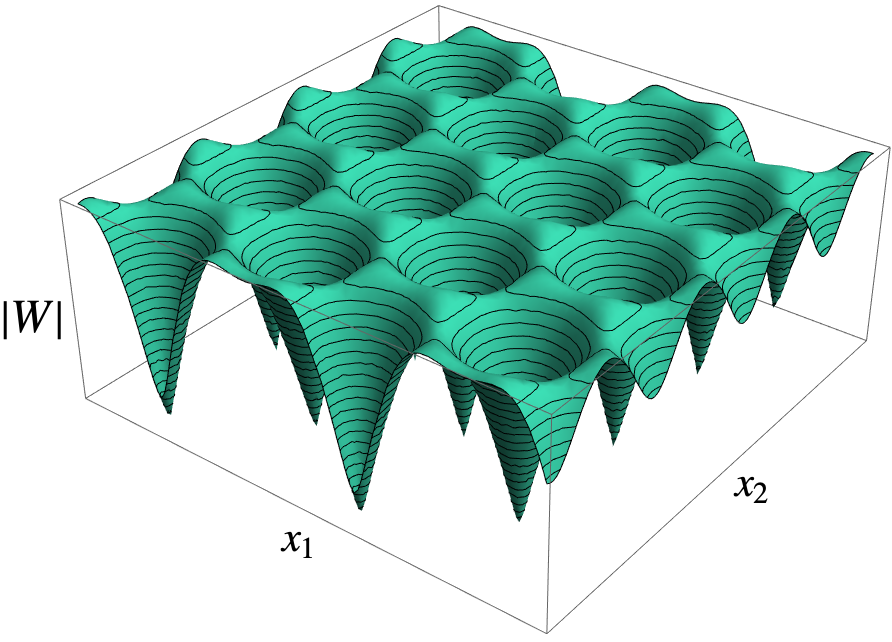
\includegraphics[width=7cm, height=5cm]{wcondensatereal.png}
        \caption{}
        \label{fig:W condensate abs}
    \end{subfigure}
    \hfill
    \begin{subfigure}[t]{0.45\textwidth}
        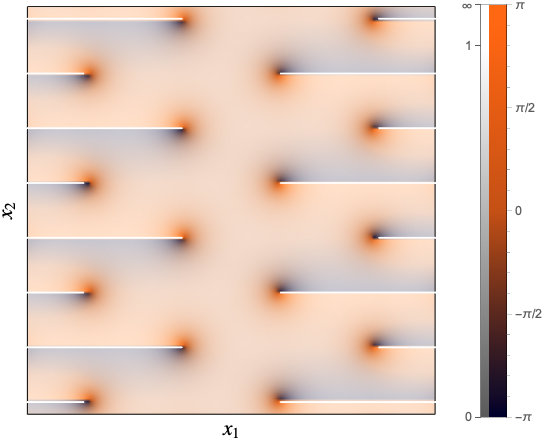
\includegraphics[width=6cm, height=5cm]{phaseplotWcondensate.png}
        \caption{}
        \label{fig:W condensate phase}
    \end{subfigure}
    \caption{\textit{Αριστερά: Η πλάτος $|W|$ ως συνάρτηση στο κάθετο στο μαγνητικό πεδίο επίπεδο. Οι ρίζες του πλάτους αντιστοιχούν στα κέντρα των εξαγωνικών δινών. Δεξιά: Το γράφημα της φάσης $\rm{Arg}(W)$, με βάση βαθμονομημένη χρωματική κλίμακα. Διαμέσου των φωτεινών ευθειών εκδηλώνεται ασυνέχεια $2\pi$ στη φάση. Οι ευθείες έχουν άκρο σε ρίζα του πλάτους και καταλήγουν στο άπειρο.}}
\end{figure}
\end{english}
\\

Εκτελώντας το μετασχηματισμό βαθμίδας
\begin{equation}\label{gauge tran in terms of the phase of W}
    A\subscr{\mu}\,\rightarrow\,A\subscr{\mu}+\frac{1}{e}\partial\subscr{\mu}\chi
\end{equation}
απαλείφεται η φάση του δυναμικού $W=|W|e\superscr{i\chi}$. 
%εντός της εξίσωσης \eqref{de for W condensation function}, και %με αντικατάσταση της \eqref{equation for Zi}, 
Τότε το ηλεκτρομαγνητικό δυναμικό $A\subscr{\mu}$ δίνεται συναρτήσει των πραγματικών ποσοτήτων $|W|,\phi$ από την έκφραση \cite{ambjornTheoryAndApplications,AMBJORN1990193}
\begin{equation}
    A\subscr{i}=\frac{1}{e}\epsilon\subscr{ij}\partial\subscr{j}(\ln|W|+2\cos\superscr{2}\theta\subscr{w}\ln\phi)\qquad i=1,2
\end{equation}
και δεν εκδηλώνει ασυνέχειες, σε αντίθεση με τη φάση $\rm{Arg}(W)=\chi$. 
Συνεπώς, σε ένα κλειστό επικαμπύλιο ολοκλήρωμα, που περιβάλλει τμήματα των ευθειών ασυνέχειας της φάσης, συνεισφέρει μόνο ο δεύτερος όρος της \eqref{gauge tran in terms of the phase of W}
\begin{equation}
    \oint (A\subscr{\mu}+\partial\subscr{\mu}\chi)dx\superscr{\mu}=\oint\partial\subscr{\mu}\chi dx\superscr{\mu}
\end{equation}
Η μαγνητική ροή διαμέσου της επιφάνειας Σ που περιβάλλεται από το βρόχο είναι κβαντισμένη και ισούται με 
%το επικαμπύλιο ολοκλήρωμα του ηλεκτρομαγνητικού δυναμικού, από %το οποίο όμως επιζεί μόνο ο προαναφερόμενος όρος
\begin{equation}\label{quantised magnetic flux}
    \int\limits_{\Sigma}F\subscr{12}d\superscr{2}x \,\,=\,\, n\Phi\subscr{o}\,\,=\,\, \oint\partial\subscr{\mu}\chi dx\superscr{\mu}
\end{equation}
όπου $n\in\mathbb{Z}$ και $\Phi\subscr{o}\equiv \frac{2\pi}{e}$ η στοιχειώδης μαγνητική ροή. Η διαφορά φάσης, που προκύπτει εκτελώντας το κλειστό επικαμπύλιο ολοκλήρωμα, είναι κβαντισμένη.\\
%επιτρέποντας την αντιστοιχία 

Αντιπαραβάλλουμε τα αποτελέσματα αυτά με τη συμπεριφορά υπεραγώγιμων υλικών εντός μαγνητικού πεδίου. 
%Συγκεκριμένα, οι περιοχές γύρω από τις οποίες το κλειστό %επικαμπύλιο ολοκλήρωμα είναι μη μηδενικό, είναι σε κοντινή %αναλογία με τις
Οι δίνες του συμπυκνώματος ζευγών Cooper σε υπεραγώγιμα υλικά απαγορεύουν τη διείσδυση στο υλικό εξωτερικού μαγνητικού πεδίου - φαινόμενο Meissner. Αντίθετα, οι δίνες του συμπυκνώματος μποζονίων $W$ ενισχύουν το αβελιανό μαγνητικό πεδίο $F\subscr{12}$, όπως φαίνεται από το θετικό πρόσημο της συνεισφοράς του συμπυκνώματος στην \eqref{equation for f12}.\\

Αυξάνοντας ακόμη περισσότερο το μαγνητικό πεδίο, 
%έξω από την περιοχή 
$F\subscr{12}\,>\,m\subscr{w}\superscr{2}$, το συμπύκνωμα διατηρεί την περιοδική μορφή του, \eqref{w condensate solution}, όπως μπορεί να αποδειχθεί διαταρακτικά 
%Η ύπαρξη των περιοδικών λύσεων 
\cite{ambjornTheoryAndApplications,AMBJORN1990193}. %αποδεικνύεται από τους Ambjorn και Olesen διαταρακτικά. 
%Η ανάλυση και τα αποτελέσματα τους είναι ανεξάρτητα των λύσεων %αυτών καθαυτών, αλλά, βασίζονται στην περιοδικότητα των |W| και %$\phi$ 
Εντός μιας κυψελίδας ικανοποιούνται οι εξισώσεις (στη βαθμίδα \eqref{gauge tran in terms of the phase of W})
\begin{english}
\begin{subequations}\label{coupled de for W and phi}
    \begin{equation}
        \partial\superscr{2}\ln|W|=-\frac{g\superscr{2}\phi\superscr{2}}{2}-2g\superscr{2}|W|\superscr{2}\qquad\partial\superscr{2}\equiv\partial\subscr{1}\superscr{2}+\partial\subscr{2}\superscr{2}
    \end{equation}
    \begin{equation}\label{de for phi2}
        \partial\superscr{2}\ln\phi\superscr{2}=\frac{g\superscr{2}}{2\cos\superscr{2}\theta\subscr{w}}(\phi\superscr{2}-v\superscr{2})+2g\superscr{2}|W|\superscr{2}
    \end{equation}
\end{subequations}
\end{english}
%Με χρήση των εξισώσεων \eqref{coupled de for W and phi}, χωρίς %να λυθούν αναλυτικά, 
Με βάση τις εξισώσεις αυτές, βρίσκουμε τη μέση τιμή ${\scriptstyle\left<\phi\superscr{2}\right>}$, ως προς την επιφάνεια $A$ μιας κυψελίδας
\begin{equation}
    \left<\phi\superscr{2}\right> \equiv \frac{1}{A}\int\subscr{A}\phi\superscr{2}d\superscr{2}x
\end{equation}
%Λόγω της θετικότητας και περιοδικότητας του $\phi\superscr{2}$, 
Oλοκληρώνοντας την \eqref{de for phi2}, η συνεισφορά του αριστερού μέλους στη μέση τιμή μηδενίζεται
\begin{equation}
    \int\subscr{A}\partial\superscr{2}\ln\phi\superscr{2}\,\,d\superscr{2}x=0
\end{equation}
Το ολοκλήρωμα της \eqref{equation for f12} και 
η εξίσωση \eqref{quantised magnetic flux} οδηγούν στη σχέση
%, δείνουν για το δεύτερο όρο τη μέση τιμή
\begin{equation}
    \frac{1}{A}\int\subscr{A}|W|\superscr{2}\,\,d\superscr{2}x=\frac{e\overline{F\subscr{12}}-m\subscr{W}\superscr{2}}{2e\superscr{2}}\qquad\overline{F\subscr{12}}\equiv\frac{2\pi n}{eA}
\end{equation}
όπου $\overline{F\subscr{12}}$ η μέση τιμή του μαγνητικού πεδίου ως προς την κυψελίδα. Εάν συνδυάσουμε τις πιο πάνω εξισώσεις, παίρνουμε 
%των παραπάνω δείνει 
\begin{equation}\label{expectation of higgs squared in a cell of periodicity}
    \left<\phi\superscr{2}\right>=v\superscr{2}\left( \frac{m\subscr{h}\superscr{2}}{m\subscr{h}\superscr{2}\sin\superscr{2}\theta\subscr{w}}-\frac{2e\cos\superscr{2}\theta\subscr{w}\overline{F\subscr{12}}}{v\superscr{2}g\superscr{2}\sin\superscr{2}\theta\subscr{w}} \right)\,\,=\,\,v\superscr{2}\, \frac{m\subscr{h}\superscr{2}-e\overline{F\subscr{12}}}{m\subscr{h}\superscr{2}-m\subscr{W}\superscr{2}},\qquad \overline{F\subscr{12}}\le \frac{m\subscr{h}\superscr{2}}{e}
\end{equation}

\section{Αποκατάσταση συμμετρίας}
Σύμφωνα με την \eqref{expectation of higgs squared in a cell of periodicity}, η μέση τιμή ${\scriptstyle\left<\phi\superscr{2}\right>}\rightarrow 0$ καθώς ${\scriptstyle e\overline{F\subscr{12}}}\rightarrow m\subscr{h}\superscr{2}$, και συνεπώς η αναμενόμενη τιμή του Higgs ελαττώνεται, ${\scriptstyle\left<\phi\right>\,}\rightarrow 0$. Στο στάδιο αυτό, συνεχίζει να εκδηλώνεται η ρήξη της ηλεκτρασθενούς συμμετρίας, αφού το πεδίο Higgs έχει μη μηδενική αναμενόμενη τιμή. Όταν ${\scriptstyle\left<\phi\superscr{2}\right>\,}=0$, η ρήξη της συμμετρίας παύει να υφίσταται, επειδή η αναμενόμενη τιμή ${\scriptstyle\left<\phi\right>\,}=0$ είναι συμμετρική ως προς τις συμμετρίες $SU(2)\,\times\,U(1)$. Η σχέση \eqref{expectation of higgs squared in a cell of periodicity}
%, αδυνατεί να διευκρινήσει την κατάσταση του μοντέλου για τιμές %${\scriptstyle e\overline{F\subscr{12}}\;\;\ge\;\;} %m\subscr{h}\superscr{2}$. 
σηματοδοτεί τη μετάβαση στην συμμετρική φάση της ηλεκτρασθενούς θεωρίας, με τα πεδία βαθμίδας να είναι τα τρία μη αβελιανά $W\superscr{i}\subscr{\mu}$ και το αβελιανό $B\subscr{\mu}$. Υπενθυμίζουμε τις σχέσεις και τους αντίστοιχους τανυστές έντασης, \eqref{tensors for electroweak gauge fields}:
\begin{english}
\begin{subequations}
    \begin{equation}
        B\subscr{\mu}=\cos\theta\subscr{w}\, A\subscr{\mu}-\sin\theta\subscr{w}\, Z\subscr{\mu}
    \end{equation}
    \begin{equation}
        W\superscr{3}\subscr{\mu}=\sin\theta\subscr{w} A\subscr{\mu}+\cos\theta\subscr{w} Z\subscr{\mu}
    \end{equation}
    \begin{equation}
        W\subscr{\mu}\superscr{1}=\frac{1}{\sqrt{2}}(W\subscr{\mu}+W\subscr{\mu}\superscr{\dagger})\qquad W\subscr{\mu}\superscr{2}=\frac{i}{\sqrt{2}}(W\subscr{\mu}-W\subscr{\mu}\superscr{\dagger})
    \end{equation}
  \begin{equation}
      B\subscr{\mu\nu}\,=\,\partial\subscr{\mu}B\subscr{\nu}-\partial\subscr{\nu}B\subscr{\mu}
  \end{equation}
  \begin{equation}
      G\superscr{i}\subscr{\mu\nu}\,=\,\partial\subscr{\mu}W\superscr{i}\subscr{\nu}-\partial\subscr{\nu}W\superscr{i}\subscr{\mu}+g\epsilon\superscr{ijk}W\superscr{j}\subscr{\mu}W\superscr{k}\subscr{\nu}
  \end{equation}
\end{subequations}
\end{english}
Η συμμετρική ως προς $SU(2)\,\times\,U(1)$ λαγκραντζιανή είναι
\begin{equation}
    \mathcal{L}=-\frac{1}{4}G\subscr{\mu\nu}\superscr{i}G\superscr{i\,\mu\nu}-\frac{1}{4}B\subscr{\mu\nu}B\superscr{\mu\nu}+|D\subscr{\mu}\phi|\superscr{2}-\lambda(\phi\superscr{2}-v\superscr{2})\superscr{2}
\end{equation}
\\

Mε βάση τις εξισώσεις \eqref{ansatz for W field}, \eqref{equation for f12}, \eqref{equation for Z12}, συμπεραίνουμε ότι, στο διάστημα ${\scriptstyle m\subscr{W}\superscr{2}\;\;\le\;\; e\overline{F\subscr{12}}\;\;\le\;\;m\subscr{h}\superscr{2}}$, οι μόνες μη μηδενικές μαγνητικές εντάσεις είναι οι ακόλουθες
\begin{english}
\begin{subequations}
\begin{equation}
    B\subscr{12}=\frac{g\,v\superscr{2}}{2\tan\theta\subscr{w}}+\frac{g}{2}\tan\theta\subscr{w}(v\superscr{2}-\phi\superscr{2})
\end{equation}
\begin{equation}
    G\subscr{12}\superscr{3}=-G\subscr{21}\superscr{3}=\frac{1}{2}g\superscr{2}\phi\superscr{2}
\end{equation}
\end{subequations}
\end{english}
Επομένως, καθώς ${\scriptstyle e\overline{F\subscr{12}}}\rightarrow m\subscr{h}\superscr{2}$, επιβιώνει μόνο το αβελιανό μαγνητικό πεδίο που συνδέεται με το υπερφορτίο $U(1)\subscr{Y}$. Συγκεκριμένα, το μαγνητικό αυτό πεδίο είναι παράλληλο με το αρχικό ηλεκτρομαγνητικό πεδίο  $U(1)\subscr{EM}$. Επειδή οι εντάσεις $G\superscr{i}\subscr{\mu\nu}$ μηδενίζονται, μηδενίζεται το μη αβελιανό μαγνητικό πεδίο $SU(2)$. 
%συνεπάγεται ότι τα πεδία $W\superscr{i}\subscr{\mu}$ δεν έχουν %κινητικούς όρους και έτσι μπορούν να απαλειφθούν από τη %λαγκρατζιανή με μετασχηματισμούς βαθμίδας. Το μαγνητικό πεδίο %λοιπόν, γίνεται εξολοκλήρου U(1)$\subscr{Y}$ ενώ 
H $SU(2)$ συνειστώσα του αρχικού ηλεκτρομαγνητικού πεδίου θωρακίζεται. Το υπερμαγνητικό πεδίο ισούται με 
\begin{equation}\label{hypermagnetic field ge to higgs mass}
    g\subscr{\y}B\subscr{12}\ge m\subscr{h}\superscr{2}\equiv 4\lambda v\superscr{2}\quad(=2\mu\superscr{2})
\end{equation}
\\

Η λαγκραντζιανή που περιγράφει τη σύζευξη του αβελιανού πεδίου βαθμίδας U(1)$\subscr{Y}$ και του βαθμωτού πεδίου Higgs 
%και της σύζευξης τους 
είναι
\begin{equation}
    \mathcal{L}=-B\subscr{\mu\nu}\superscr{2}+\underbrace{|(\partial\subscr{\mu}-i\frac{1}{2}g\subscr{\y}B\subscr{\mu})\phi|\superscr{2}+\mu\superscr{2}|\phi|\superscr{2}}\subscr{\mathcal{L}\subscr{o}}-\lambda(\phi\superscr{*}\phi)\superscr{2}-\lambda v\superscr{2},\qquad (\mu\superscr{2}=2\lambda v\superscr{2})
\end{equation}
όπου το υπερφορτίου του Higgs ισούται με $Y{\scriptstyle=\frac{1}{2}}$ και $g\subscr{\y}{\scriptstyle=} g\tan\theta\subscr{w}$ η σταθερά σύζευξης του U(1)$\subscr{Y}$ πεδίου βαθμίδας. Το δυναμικό $B\subscr{\mu}$ 
%πρέπει να ικανοποιεί τις εξισώσεις για σταθερό πεδίο στις %εγκάρσιες διευθύνσεις $x\subscr{1}-x\subscr{2}$
%\begin{equation}
%    \text{constant}=B\subscr{\mu\nu}=\partial\subscr{\mu}B\subs%cr{\nu}-\partial\subscr{\nu}B\subscr{\mu}
%\end{equation}
στη βαθμίδα Landau δίδεται από την έκφραση
\begin{equation}
    B\subscr{\mu}=x\subscr{1}B\subscr{12}\de\subscr{\mu 2}\qquad\left(\Rightarrow B\subscr{\mu}\superscr{2}=-(B\subscr{12}x\subscr{1})\superscr{2}\right)
\end{equation}
όπου $B\subscr{12}$ το σταθερό μαγνητικό πεδίο.
%Απομονώνοντας τους όρους $\mathcal{L}\subscr{o}$, 
Οι εξισώσεις κίνησης για το πεδίο Higgs, 
για $\phi \sim 0$ είναι
\begin{equation}\label{equations of motion for higgs around phi=0}
    \frac{\de \mathcal{L}\subscr{o}}{\de \phi\superscr{*}}-\partial\subscr{\mu}\frac{\de\mathcal{L}\subscr{o}}{\de(\partial\subscr{\mu}\phi\superscr{*})}=0\quad\Rightarrow\quad \partial\superscr{2}\phi=\left(-\frac{g\subscr{\y}\superscr{2}}{4}(B\subscr{12}x\subscr{1})\superscr{2}-ig\subscr{\y}B\subscr{\mu}\partial\subscr{\mu}+\mu\superscr{2}\right)\phi
\end{equation}
Χωρίζοντας μεταβλητές $\phi=e\superscr{iE\subscr{n}x\subscr{o}}\phi\subscr{n}(x\subscr{1},x\subscr{2},x\subscr{3})$, 
%η εξίσωση \eqref{equations of motion for higgs around phi=0} %γράφεται ως η εξίσωση ιδιοτιμών
παίρνουμε
\begin{equation}\label{eigenvalue equation from eom for higgs}
    E\subscr{n}\superscr{2}\phi\subscr{n}=-\left( \partial\superscr{2}\subscr{i} -g\subscr{\y}\superscr{2}\left(\frac{B\subscr{12}x\subscr{1}}{2}\right)\superscr{2}-ig\subscr{\y}(B\subscr{12}x\subscr{1})\partial\subscr{2}+\mu\superscr{2} \right)\phi\subscr{n}
\end{equation}
%Περαιτέρω απλοποίηση γίνεται, αναγνωρίζοντας ότι, 
Οι λύσεις πρέπει να είναι αναλλοίωτες ως προς μεταφορές στις διευθύνσεις $x\subscr{2},\,x\subscr{3}$. 
%αφού δεν εμφανίζονται στην εξίσωση ιδιοτιμών. 
Επομένως θέτουμε 
\begin{equation}
    \phi\subscr{n}\sim e\superscr{ip\subscr{2}x\subscr{2}}e\superscr{ip\subscr{3}x\subscr{3}}\Tilde{\phi}\subscr{n}(x\subscr{1})
\end{equation}
Η \eqref{eigenvalue equation from eom for higgs} παίρνει τη μορφή
\begin{equation}\label{eigenvalue equation from eom for higgs simplified}
    E\subscr{n}\superscr{2}\Tilde{\phi}\subscr{n}=\left(p\subscr{3}\superscr{2}-\mu\superscr{2}-\partial\subscr{1}\superscr{2}+\left(\frac{g\subscr{\y}B\subscr{12}}{2}x\subscr{1}-p\subscr{2}\right)\superscr{2}\right)\Tilde{\phi}\subscr{n}
\end{equation}
Οι τελευταίοι δύο όροι στα δεξιό μέλος της \eqref{eigenvalue equation from eom for higgs simplified} διαγονοποιούνται με χρήση των ιδιοσυναρτήσεων ενός αρμονικού ταλαντωτή στην διεύθυνση $x\subscr{1}$, συχνότητας $\frac{g\subscr{\y}B\subscr{12}}{2}$. Οι αντίστοιχες ιδιοτιμές είναι
\begin{equation}
    g\subscr{\y}B\subscr{12}\left( n+\frac{1}{2} \right)
\end{equation}
Ο ακέραιος αριθμός $n$ χαρακτηρίζει τις στάθμες Landau. Η ενέργεια της χαμηλότερης στάθμης είναι
\begin{equation}\label{higgs energy lowest landau level around phi=0}
    E\superscr{2}\subscr{o}=p\subscr{3}\superscr{2}-\mu\superscr{2}+\frac{g\subscr{\y}B\subscr{12}}{2}
\end{equation}
\\

Το υπερμαγνητικό πεδίο ικανοποιεί τη σχέση \eqref{hypermagnetic field ge to higgs mass} και άρα η ενεργός μάζα του πεδίου Higgs που απορρέει από την εξίσωση διασποράς \eqref{higgs energy lowest landau level around phi=0} είναι θετική. Επομένως, η συμμετρική κατάσταση ${\scriptstyle\phi=0}$ είναι ευσταθής όταν το μαγνητικό πεδίου παίρνει τιμές στο διάστημα \eqref{hypermagnetic field ge to higgs mass}. Η ηλεκτρασθενής συμμετρία επαναφέρεται.\\ 

Το υπερμαγνητικό πεδίο συζεύγνυται διαφορετικά με την ύλη. Αντικαθιστούμε τη %αλλαγές αντικατοπτρίζονται από την αντικατάσταση της 
σταθερά σύζευξης του ηλεκτρομαγνητισμού
\begin{equation}
    e\equiv \frac{gg\subscr{\y}}{\sqrt{g\superscr{2}+g\subscr{\y}\superscr{2}}},\qquad \left(g=\frac{g\subscr{\y}}{\tan\theta\subscr{w}}\right)
\end{equation}
με την υπερμαγνητική σταθερά σύζευξης, $e\rightarrow g\subscr{\y}=\frac{e}{\cos\theta\subscr{w}}$. Για παράδειγμα, η μάζα μιας ακραίας οπής ελαττώνεται κατά $\cos\theta\subscr{w}$:
\begin{equation}
    M\subscr{e}=\sqrt{\frac{\pi}{G}}\frac{Q}{e}\,\rightarrow\,\sqrt{\frac{\pi}{G}}\frac{Q}{g\subscr{\y}}=\sqrt{\frac{\pi}{G}}\frac{Q}{e}\cos\theta\subscr{w}
\end{equation}

\begin{comment}
\section*{Προχειρο}
Η συγκέντρωση επηρεάζει την αναμενόμενη τιμή του Higgs $\left<\phi\right>$ μεταξύ των κατωφλίων $m\subscr{w}\superscr{2}\le|F|\le m\subscr{h}\superscr{2}$ και παρουσιάζεται στο άρθρο συναρτήσει της αναμενόμενης τιμής $|\left<\phi\subscr{o}\right>|\equiv v$ του συνηθισμένου κενού
\begin{equation}
    |\left<\phi\right>|\superscr{2} = v\superscr{2}\frac{m\subscr{h}\superscr{2}-|F|}{m\subscr{h}\superscr{2}-m\superscr{2}\subscr{w}}.\qquad m\subscr{w}\superscr{2}\le|F|\le m\subscr{h}\superscr{2}
\end{equation}
Είναι εμφανές ότι, αν και το Higgs δεν αλληλεπιδρά ηλεκτρομαγνητικά, επηρεάζεται έμμεσα μέσω της αλληλεπίδρασης των spin-1 μποζονίων με το εξωτερικό μαγνητικό πεδίο. Οι φυσικές συνέπειες της αύξησης των spin-1 σωματιδίων επεκτείνονται και στο ίδιο το μαγνητικό πεδίο \cite{AMBJORN1990193,ambjornTheoryAndApplications}. Η ευσταθής λύση του πεδίου στο διάστημα $|F|\ge m\superscr{2}\subscr{h}$ ($r\le r\subscr{h}$) καταλήγει να είναι ένα καθαρά αβελιανό πεδίο $\text{U(1)}\subscr{Y}$. Με χρήση του συμβολισμού της ενότητας \ref{section local gauge theory}, όπου $G\superscr{i}\subscr{\mu\nu}$ και $B\subscr{\mu\nu}$ οι τανυστές που αντιστοιχούν στα πεδία βαθμίδας της συμμετρικής φάσης της ηλεκτρασθενούς θεωρίας $SU(2)\times U(1)$, οι ευσταθείς λύσεις είναι \cite{AMBJORN1990193,ambjornTheoryAndApplications}
\begin{equation}
    \left<\phi\right>\rightarrow 0\,\Rightarrow\,\left\{ \begin{array}{l} G\superscr{i}\subscr{\mu\nu} \sim \left<\phi\right> \rightarrow 0 \\ B\subscr{\mu\nu}\ne 0 \end{array} \right.
\end{equation}
Μέσω του υπερφορτίου ½, το πεδίου Higgs συζεύγνυται με το πλέον υπερμαγνητικό πεδίο και η ενέργεια του αναβαθμίζεται με τη συνεισφορά του επιπέδου Landau. Για το χαμηλότερο επίπεδο n=0, το υπερμαγνητικό πεδίο συνεισφέρει θετικά στην ενεργό μάζα του πεδίου και αποδίδει ένα θετικό τετραγωνικό ως προς το πεδίο όρο εντός του ενεργού δυναμικού
\begin{equation}
    V(\phi\superscr{\dagger}\phi)\,=\, (-\mu\superscr{2}+\frac{|F|}{2})\,|\phi|\superscr{2}+\lambda|\phi|\superscr{4}
\end{equation}
Όπως αναφέρθηκε στην προηγούμενη ενότητα, πέραν της κρίσιμης τιμής της έντασης $|F|\ge 2\mu\superscr{2}\equiv m\superscr{2}\subscr{h}$ ($r\le r\subscr{h}$) το δυναμικό ελαχιστοποιείται μόνο από πεδίο με μέση τιμή $\left<\phi\right>=0$ και επομένως η ευσταθής πλέον κατάσταση είναι αυτή με την αποκατάσταση της συμμετρία. το διάστημα $r<r\subscr{h}$, είναι επακόλουθο ότι 
\end{comment}

\section{Καταστολή μηχανισμού Higgs}
Η αναμενόμενη τιμή του πεδίου Higgs ελαττώνεται καθώς αυξάνεται η ένταση του μαγνητικού πεδίου μέχρι να μηδενιστεί εντελώς στην περιοχή $r\subscr{e}\le r \le r\subscr{h}$. Οι μάζες των φερμιονίων μηδενίζονται.
%σωματιδίων ύλης (επακόλουθο της σύζευξης με το πεδίο $\phi$ %στην ενότητα \ref{section mass for fermions} και του ασύμετρου %κενού) είναι ανάλογες της συνήθης μέσης τιμής %$\left<\phi\right>\ne 0$, αναμένεται να μηδενιστούν. Η μάζα των %φερμιονικών πεδίων (μέσω του μηχανισμού Higgs) καταστέλλεται, %και τα πεδία καθιστώνται άμαζα εντός του καθορισμένου %διαστήματος. 
Έτσι, γίνονται πιο έντονες οι κβαντικές διακυμάνσεις των πεδίων αυτών και ενισχύεται το φαινόμενο της
%Κβαντικές διακυμάνσεις φερμιονικών πεδίων κοντά στον ορίζοντα %της μελανής οπής οδηγούν σε 
%Τα φερμιονικά πεδία θετικής ενέργειας που διαδίδονται προς το %εξωτερικό της κορώνας με την ταχύτητα του φωτός (μέχρι να %αποκτήσουν ξανά μάζα εκτός της κορώνας), συνεισφέροντας στην 
ακτινοβολίας Hawking. Στην ενίσχυση της ακτινοβολίας συνεισφέρει ο εκφυλισμός της χαμηλότερης στάθμης Landau,
%. Ο εκφυλισμός του ενεργειακού επιπέδου διαφέρει ελαφρώς από %αυτόν της ενότητας \ref{section LLL degeneracy} αλλά %εξακολουθεί 
ο οποίος είναι ανάλογος του μαγνητικού φορτίου Q. 
%Η διαφορά οφείλεται στο κλασματικό υπερφορτίο των φερμιονικών %πεδίων. 

\section{Υπερφορτίο και εκφυλισμός}
Στην ενότητα \ref{section LLL degeneracy}, προσδιορίσαμε τον εκφυλισμό της χαμηλότερης στάθμης Landau LLL για σωματίδια με φορτίο ίσο με ακέραιου πολλαπλάσιο του φορτίου του ηλεκτρονίου. %Ο εκφυλισμός του LLL της ενότητας \ref{section LLL degeneracy} %αναθεωρείται 
Στην περίπτωση υπερμαγνητικού πεδίου, όπως συμβαίνει εντός της ηλεκτρασθενούς κορώνας, θα πρέπει να λάβουμε υπόψη το υπερφορτίο κάθε σωματιδίου. 
%αναπαράστασης της SU(3)$\times$SU(2)$\times$U(1) ομάδας. 
Τα υπερφορτία φαίνονται στον πίνακα \ref{tab:table with particles and su3, su2 representations}. 
%Πέραν του εκφυλισμού, 
%Θα εξετάσουμε επίσης τη συμπεριφορά φερμιονικών πεδίων 
%εντός του συνδυασμού υπερμαγνητικού και βαρυτικού πεδίου έξω %από 
στην εξωτερική περιοχή μιας μελανής οπής. Στην επόμενη ενότητα μελετούμε τις λύσεις της εξίσωσης Dirac στην παρουσία βαρυτικού και ηλεκτρομαγνητικού πεδίου.

\section{Εξίσωση Dirac}\label{section dirac equation in gravity}
Η γενίκευση της εξίσωσης Dirac σε καμπύλους χώρους γίνεται με την χρήση κατάλληλης συναλλοίωτης παραγώγου. Αυτή ορίζεται ως ακολούθως 
%απαίτηση για παραγώγους σπινορικών πεδίων με τανυστικούς %μετασχηματισμούς οδηγεί στον ορισμό
\begin{equation}
    \nabla\subscr{\mu}\,\equiv\,\partial\subscr{\mu}+\frac{1}{4}\omega\subscr{\mu ab}\gamma\superscr{a}\gamma\superscr{b}
\end{equation}
όπου $\omega\subscr{ab\mu}$ η σπινορική σύνδεση (spin connection) \cite{Carroll2003-CARSAG-3}
\begin{equation}\label{spin connection}
    \omega\subscr{\mu ab}\,\equiv\,e\subscr{\nu a}e\superscr{\lambda}\subscr{\;\;b}\Gamma\superscr{\nu}\subscr{\mu\lambda}-e\superscr{\lambda}\subscr{\;\;b}\,\partial\subscr{\mu}e\subscr{\lambda a}
\end{equation}
και $\gamma\superscr{a}$ οι πίνακες Dirac 
%του επίπεδο χώρου Minkowski 
με τις αντιμεταθετικές σχέσεις 
\begin{equation}\label{gamma anticommutator 4d}
    \{ \gamma\superscr{a},\gamma\superscr{b} \}\,=\,2\,\mink[1]{a}{b}\,\mathbf{I\subscr{4}}
\end{equation}
%και οι τετράδες (vierbein) διανυσματικών πεδίων (ένα για κάθε %τιμή του δείκτη $a$) 
Τα πεδία $e\subscr{\mu}\superscr{\;\;a}$ συνδέονται με τη μετρική
%καθορίζουν εφαπτόμενες ορθοκανονικές βάσεις σε κάθε σημείο της %πολλαπλότητας με την μετρική 
$\g{\mu}{\nu}$ με βάση τη σχέση \cite{Carroll2003-CARSAG-3}
\begin{equation}
    \g{\mu}{\nu}=e\subscr{\mu}\superscr{\;\;a}e\subscr{\nu}\superscr{\;\;b}\mink{a}{b},\qquad \mink{a}{b}:=\text{diag}(-1,+1,+1,+1)
\end{equation}
%καθώς επίσης ισχύει η εξής διαφοροποίηση στους κανόνες που %ακολουθούν 
Οι λατινικοί και οι ελληνικοί δείκτες ανεβοκατεβαίνουν ως εξής
\begin{equation}\label{vierbein identity manipulating indices}
    e\superscr{\mu}\subscr{\;\;a}=\g[1]{\mu}{\nu}\mink{a}{b}e\superscr{\;\;b}\subscr{\nu}
\end{equation}
\\

Όταν το φερμιονικό πεδίο αλληλεπιδρά με ένα 
%φορτισμένου (q) σπινορικού πεδίου με 
ηλεκτρομαγνητικό πεδίο 
%\eqref{vector potential for monopole in curvilinear coo} όπου %$Q=2s\subscr{o}$ είναι το ακέραιο μαγνητικό φορτίο
%\begin{equation}
%    A\subscr{\mu}=\frac{s\subscr{o}}{e}\cos\theta\,\,\de\subscr%{\mu\phi}
%\end{equation}
%εγκαθίσταται στον ορισμό της 
η πιο πάνω συναλλοίωτη παράγωγος ανάγεται στην 
%με το συνηθισμένο τρόπο
\begin{equation}
    D\subscr{\mu}\,\equiv\,\partial\subscr{\mu}+\frac{1}{4}\omega\subscr{\mu ab}\gamma\superscr{a}\gamma\superscr{b}+iqA\subscr{\mu}
\end{equation}
Η εξίσωση Dirac για άμαζο φερμιονικό πεδίο $\chi$ είναι
\begin{equation}\label{general dirac equation}
    ie\superscr{\mu}\subscr{\;\;a}\gamma\superscr{a}D\subscr{\mu}\chi=0
\end{equation}
\\

Γράφουμε τη μετρική \eqref{ReissnerNordmetric} στη βοηθητική μορφή
\begin{equation}
    ds\superscr{2}\,=\,F(r)\left( -dt\superscr{2}+dx\superscr{2} \right)+r\superscr{2}(x)d\Omega\superscr{2}\,,\qquad F(r)=\left(1-\frac{2G M}{r}+\frac{G\pi Q^2}{e^2r^2}\right)
\end{equation}
%με την αντικατάσταση της ακτινικής συνεταγμένης r
όπου
\begin{equation}
    dx\,\equiv\,\frac{dr}{F(r)}
\end{equation}
%Το γωνιακό κομμάτι της μετρικής έχει τον συντελεστή %$r\superscr{2}$ ως προς τον οποίο παραγοντοποιείται η μετρική. %Ο καθολικός θετικός παράγοντας της μετρικής είναι ένας τοπικός %παράγοντας επανακλιμάκωσης (Weyl transformation) της μετρικής %και επιτρέπεται να αγνοηθεί αφού 
Η άμαζη εξίσωση Dirac είναι αναλλοίωτη ως προς τοπικούς σύμμορφους μετασχηματισμούς Weyl. Για τον λόγο αυτό, μπορούμε να αμελήσουμε έναν ολικό σύμμορφο παράγοντα, θέτοντας το συντελεστή του γωνιακού μέρους της μετρικής ίσο με τη μονάδα: 
%Το γωνιακό κομμάτι της μετρικής είναι πλέον ανεξάρτητο των t %και x
\begin{equation}\label{metric with a weyl factor for the t-x part}
     ds\superscr{2}\,=\,e\superscr{2\rho}\left( -dt\superscr{2}+dx\superscr{2} \right)+d\Omega\superscr{2},\qquad  e\superscr{2\rho(x)}\equiv\frac{F(r)}{r\superscr{2}}
\end{equation}
Με βάση τη μετρική \eqref{metric with a weyl factor for the t-x part}, οι μη μηδενικές συνιστώσες του πεδίου $e\superscr{\;\;a}\subscr{\mu}$ είναι
\begin{equation}
    e\superscr{\;\;0}\subscr{t}=e\superscr{\,\rho},\quad  e\superscr{\;\;1}\subscr{x}=e\superscr{\,\rho},\quad
    e\superscr{\;\;2}\subscr{\theta}=1,\quad
    e\superscr{\;\;3}\subscr{\theta}=\sin\theta
\end{equation}
Βρίσκουμε στη συνέχεια τα μη μηδενικά στοιχεία της σπινορικής σύνδεσης \eqref{spin connection}
\begin{equation}
    \omega\subscr{t10}=-\omega\subscr{t01}=\frac{d\rho}{dx}\equiv\rho',\quad\omega\subscr{\phi32}=-\omega\subscr{\phi23}=\cos\theta
\end{equation}
Στον δισδιάστατο χωρόχρονο $tx$, οι πίνακες Dirac ικανοποιούν τις αντιμεταθετικές σχέσεις
\begin{equation}
    \{ \bar{\gamma}\superscr{a},\bar{\gamma}\superscr{b} \}\,=\,2\,\mink[1]{a}{b}\,\mathbf{I\subscr{2}},\qquad \mink{a}{b}:=\text{diag}(-1,+1)
\end{equation}
που ικανοποιούνται από τους πίνακες 
\begin{equation}\label{gamma 2d repre t-x}
    \bar{\gamma}\superscr{0}=i\sigma\superscr{x}\qquad\bar{\gamma}\superscr{1}=\sigma\superscr{\y}
\end{equation}
Για τη σφαίρα, οι αντίστοιχες σχέσεις είναι
\begin{equation}
     \{ \bar{\gamma}\superscr{a},\bar{\gamma}\superscr{b} \}\,=\,2\,\de\superscr{ab}\,\mathbf{I\subscr{2}},\qquad \de\superscr{ab}:=\text{diag}(+1,+1)
\end{equation}
και
\begin{equation}\label{gamma 2d repre theta-phi}
    \bar{\gamma}\superscr{1}=\sigma\superscr{x}\qquad\bar{\gamma}\superscr{2}=\sigma\superscr{\y}
\end{equation}
Οι δυσδιάστατες αναπαραστάσεις, \eqref{gamma 2d repre t-x} και \eqref{gamma 2d repre theta-phi}, συνδυάζονται στις ακόλουθες τετραδιάστατες \cite{Maldacena2018TraversableWI} 
\begin{equation}\label{gamma 4d repre}
    \gamma\superscr{0} = i\sigma\superscr{x}\otimes\mathbf{I}\subscr{2}\qquad
    \gamma\superscr{1} = \sigma\superscr{\y}\otimes\mathbf{I}\subscr{2}\qquad
    \gamma\superscr{2} = \sigma\superscr{z}\otimes\sigma\superscr{x}\qquad
    \gamma\superscr{3} = \sigma\superscr{z}\otimes\sigma\superscr{\y}
\end{equation}
που ικανοποιούν τις σχέσεις \eqref{gamma anticommutator 4d}.
Στην αναπαράσταση \eqref{gamma 4d repre} ο  χειραλικός τελεστής %χειραλικότητας ορίζεται ως το εξωτερικό γινόμενο
είναι
\begin{equation}\label{gamma 5 repre in 4d}
    \gamma\superscr{5}=i\gamma\superscr{0}\gamma\superscr{1}\gamma\superscr{2}\gamma\superscr{3}=i(-\sigma\superscr{z}\otimes i\sigma\superscr{z})=\sigma\superscr{z}\otimes\sigma\superscr{z}
\end{equation}
Οι λύσεις της \eqref{general dirac equation} αποτελούν ιδιοκαταστάσεις του \eqref{gamma 5 repre in 4d} με ιδιοτιμές +1 και -1, και αντιστοιχούν σε δεξιόστροφα και αριστερόστροφα φερμιονικά πεδία. Αντικαθιστώντας τα πιο πάνω στην \eqref{general dirac equation}, η εξίσωση Dirac παίρνει τη μορφή
\begin{equation}
    \left[e\superscr{-\rho}\left(i\sigma\superscr{x}\partial\subscr{t}+\sigma\superscr{\y}(\partial\subscr{x}+\frac{\rho'}{2})\right)\otimes \mathbf{I}\subscr{2} \;+\; \sigma\superscr{z}\otimes\left( \sigma\superscr{\y}\frac{\partial\subscr{\phi}+iqA\subscr{\phi}}{\sin\theta} + \sigma\superscr{x}\left(\partial\subscr{\theta}+\frac{\cot\theta}{2}\right) \right) \right]\chi=0
\end{equation}
Υπενθυμίζουμε ότι στην περίπτωση μαγνητικού μονοπολικού πεδίου η μόνη μη μηδενική συνιστώσα του δυναμικού είναι η $A_\phi$.

\section{Λύσεις Dirac}\label{sec:dirac solutions in magnetic mon field}
Οι τετραδιάστατες λύσεις της εξίσωσης \eqref{general dirac equation} σε χωροχρόνο της μορφής $\mathbf{M}=\mathbb{R}\superscr{1,1}\times S\superscr{2}$ ανάγονται σε τανυστικό γινόμενο δύο δισδιάστατων σπινόρων $\psi$ και $\eta$ \cite{Maldacena2018TraversableWI}
\begin{equation}\label{dirac solution ansatz}
    \chi\subscr{ij}(t,x,\theta,\phi)\,=\,e\superscr{-\rho(x)}\psi\subscr{i}(t,x)\otimes\eta\subscr{j}(\theta,\phi),\qquad i,j=1,2
\end{equation}
%Εφαρμόζοντας το ansatz \eqref{dirac solution ansatz} 
Η εξίσωση Dirac ανάγεται σε σύστημα δύο ασύζευκτων διαφορικών εξισώσεων
\begin{english}
\begin{subequations}
  \begin{equation}
    \label{dirac t-x de}
    \left[i\sigma\superscr{x}\partial\subscr{t}+\sigma\superscr{\y}\partial\subscr{x}\right]\psi=0
  \end{equation}
  \begin{equation}
    \label{dirac θ-φ de}
        \left[\sigma\superscr{\y}\frac{\partial\subscr{\phi}+iqA\subscr{\phi}}{\sin\theta} + \sigma\superscr{x}\left(\partial\subscr{\theta}+\frac{\cot\theta}{2}\right)\right]\eta=0
  \end{equation}
\end{subequations}
\end{english}
Οι δύο εξισώσεις της \eqref{dirac θ-φ de}, μια για κάθε συνιστώσα του σπίνορα $\eta$, 
\begin{equation}
    \eta\,:=\,\left( \begin{array}{c} \eta\subscr{1}\\ \eta\subscr{2} \end{array} \right)
\end{equation}
ικανοποιούνται με χρήση των ιδιοκαταστάσεων Haldane \eqref{monomial eigenfunction}. Για φερμιονικό πεδίο με θετικό φορτίο $q=e$, η λύση είναι
\begin{equation}
    \eta\subscr{+}\equiv\left( \begin{array}{c} \eta\subscr{1}\\ 0 \end{array} \right),\qquad\quad
    \eta\subscr{1}= \left(\cos\frac{\theta}{2}\right)\superscr{s\subscr{o}-\frac{1}{2}+m}\left(\sin\frac{\theta}{2}\right)\superscr{s\subscr{o}-\frac{1}{2}-m}e\superscr{- im\phi}
\end{equation}
Για αρνητικό φορτίο $q=-e$ παίρνουμε
\begin{equation}
    \eta\subscr{-}\equiv\left( \begin{array}{c} 0\\ \eta\subscr{2} \end{array} \right),\qquad\quad
    \eta\subscr{2}= \left(\cos\frac{\theta}{2}\right)\superscr{s\subscr{o}-\frac{1}{2}+m}\left(\sin\frac{\theta}{2}\right)\superscr{s\subscr{o}-\frac{1}{2}-m}e\superscr{im\phi}
\end{equation}
Οι σπίνορες αυτοί έχουν καλά ορισμένη χειραλικότητα, $\sigma\superscr{z}\eta\subscr{\pm}=\pm\eta\subscr{\pm}$, όπως φένεται από τη δράση του τελεστή χειραλικότητας 
στην αναπαράσταση της σφαίρας $S\superscr{2}$, $\mathbf{I\subscr{2}}\otimes\sigma\superscr{z}$. Αρνητικά (θετικά) φορτισμένα φερμιονικά πεδία περιγράφονται με βάση τον σπίνορα $\eta\subscr{-}$ ($\eta\subscr{+}$). 
%σπίνορα στη σφαίρα $S\superscr{2}$. 
Για πεδία με κλασματικό φορτίο η ανάλυση είναι ποιοτικά παρόμοια.\\

%με διαφορά στον εκφυλισμό των ιδιοκαταστάσεων Haldane. 
Η ανάλυση της εξίσωσης \eqref{dirac t-x de} γίνεται με παρόμοιο τρόπο. Συναρτήσει των συνιστωσών του $\psi$, η \eqref{dirac t-x de} ανάγεται στις
\begin{english}
\begin{subequations}
  \begin{equation}
    \label{t-x de for psi1}
        \left( \partial\subscr{t}+\partial\subscr{x} \right)\psi\subscr{1}=0
    \end{equation}
  \begin{equation}
    \label{t-x de for psi2}
        \left( \partial\subscr{t}-\partial\subscr{x} \right)\psi\subscr{2}=0
  \end{equation}
\end{subequations}
\end{english}
%όπου φανερώνεται η μορφή των λύσεων
Οι λύσεις έχουν τη μορφή
\begin{english}
\begin{subequations}\label{dirac solutions t-x}
  \begin{equation}
    \label{t-x solution for psi1}
        \psi\subscr{1}:=\psi\subscr{1}(t-x)
    \end{equation}
  \begin{equation}
    \label{t-x solution for psi2}
        \psi\subscr{2}:=\psi\subscr{2}(t+x)
  \end{equation}
\end{subequations}
\end{english}
Η συνάρτηση \eqref{t-x solution for psi1} περιγράφει ένα δεξιόστροφο, εξερχόμενο πεδίο. 
%κινούμενο προς αύξουσες τιμές της συντεταγμένης x (r), επομένως %είναι δεξιοκίνητο και απομακρύνεται από τον ορίζοντα (out). 
Αντίθετα, η \eqref{t-x de for psi2} περιγράφει αριστερόστροφα, εισερχόμενα πεδία. 
%που κινούνται προς φθίνουσες τιμές της x (r), καταλήγοντας %εντός του ορίζοντα (in). 
Οι ιδιοκαταστάσεις του τελεστή χειραλικότητας $\sigma\superscr{z}\otimes\mathbf{I\subscr{2}}$, στην αναπαράσταση του $\mathbb{R}\superscr{1,1}$, ικανοποιούν $\sigma\superscr{z}\psi\subscr{\pm}=\pm\psi\subscr{\pm}$ και προκύπτουν από τις λύσεις \eqref{dirac solutions t-x}
\begin{equation}
    \psi\subscr{+}=\left( \begin{array}{c}\psi\subscr{1}(t-x)\\0\end{array} \right), \qquad \psi\subscr{-}=\left( \begin{array}{c}0\\ \psi\subscr{2}(t+x)\end{array} \right)
\end{equation}
\\

Το γινόμενο \eqref{dirac solution ansatz} των δύο δισδιάστατων σπινόρων $\eta$ και $\psi$ δίνει το τετραδιάστατο φερμιονικό πεδίο. Η χειραλικότητα καθορίζεται με βάση την αναπαράσταση της ομάδας $SU(3)\otimes SU(2)\otimes U(1)$. 
%Το γινόμενο των δυσδιάστατων χειραλικοτήτων των $\eta$ και %$\psi$ πρέπει επομένως να συμφωνεί με την τετραδιάστατη %χειραλικότητα. 
Για παράδειγμα, στην περίπτωση ενός αρνητικά φορτισμένου, αριστερόστροφου πεδίου $\chi\subscr{L}$, ο σπίνορας στην $S\superscr{2}$ είναι ο $\eta\subscr{-}$ και επομένως
\begin{equation}
    \gamma\superscr{5}\chi\subscr{L}=(\sigma\superscr{z}\otimes\sigma\superscr{z})(\psi\otimes\eta\subscr{-})\;\Rightarrow\;-\chi\subscr{L}=(\sigma\superscr{z}\psi)\otimes(-\eta\subscr{-})
\end{equation}
Συνεπώς ο σπίνορας $\psi$ είναι ίσος με $\psi\subscr{+}$, και έτσι το πεδίο $\chi\subscr{L}$ είναι εξερχόμενο. 
%κινείται προς αύξουσα x και διαφεύγει της οπής (out). 
Τα πιο πάνω συνοψίζονται στον ακόλουθο κανόνα για τον προσδιορισμό των εξερχόμενων και εισερχόμενων πεδίων
\begin{equation}\label{rule for out in fields}
    \text{sign}(h\subscr{\chi}\cdot q) =\left\{\begin{array}{c} +\quad (\text{out})\\ -\quad (\text{in})\end{array}\right.
\end{equation}
όπου $h\subscr{\chi}$ και $q$ η χειραλικότητα 
%του φερμιονικού πεδίου προς εξέταση 
και το φορτίο του αντίστοιχα. Λόγω του υπερμαγνητικού πεδίου εντός της ηλεκτρασθενούς κορώνας, χρησιμοποιούμε το υπερφορτίο.

\begin{table}[t]
    \centering
    \begin{tabular}{|c|c|}
    \hline
    SU(3)$\otimes$SU(2)$\otimes$U(1) & In-Out\\
    \hline
    (3,2,1/6)&Q-\\
    \hline
    (3,1,2/3)&-2Q\\
    \hline
    (3,1,-1/3)&Q-\\
    \hline
    (1,2,-1/2)&-Q\\
    \hline
    (1,1,-1)&Q-\\
    \hline
    \end{tabular}
    \caption{\textit{Ο συνολικός εκφυλισμός κάθε αναπαράστασης. Για τα εξερχόμενα φερμιόνια η παύλα είναι αριστερά και δεξιά για τα εισερχόμενα.}}
    \label{table: out-in fields and degeneracy for each representation}
\end{table}

\section{Εισερχόμενα - Εξερχόμενα φερμιόνια}
Ο εκφυλισμός κάθε αναπαράστασης της ομάδας $SU(3)\otimes SU(2)\otimes U(1)$ εντός της κορώνας ισούται με το γινόμενο του υπερφορτίου, του αριθμού των πεδίων και του μαγνητικού φορτίου $Q$. Για παράδειγμα, στα δεξιόστροφων up quarks αντιστοιχεί εκφυλισμός 2Q, με βάση την \eqref{rule for out in fields} είναι εισερχόμενα \cite{Maldacena_2021}. Οι αναπαραστάσεις ταξινομούνται στον πίνακα \ref{table: out-in fields and degeneracy for each representation}. Υπάρχουν $3Q$ εκφυλισμένες καταστάσεις που αντιστοιχούν σε εξερχόμενα πεδία. Επειδή υπάρχουν τρεις οικογένειες στο καθιερομένο πρότυπου, ο εκφυλισμός των εξερχόμων πεδίων είναι
\begin{equation}\label{degeneracy of out fields}
    \text{Εκφυλισμός "out" καταστάσεων}=9Q
\end{equation}

\section{Ρθμός εκπομπής ενέργειας μελανών οπών}\label{sec:energy radiation of one dimensional fermionic model}
Όταν τα εξερχόμενα πεδία του πίνακα \ref{table: out-in fields and degeneracy for each representation} 
%(και οι υπόλοιπες δύο οικογένειες), εφόσον δημιουργούνται 
παραχθούν εξαιτίας κβαντικών διακυμάνσεων κοντά στον ορίζοντα, διαδίδονται προς το άπειρο μεταφέροντας την ενέργεια (μάζα) που χάνει η οπή. 
%βάση του νόμου της ολικής διατήρησης. 
Εντός της ηλεκτρασθενούς κορώνας, η σχέση διασποράς των άμαζων φερμιονικών πεδίων δίνεται από τη σχέση \eqref{spinor energy magnetic field}
\begin{equation}\label{massless spinor energy magnetic field}
    E\superscr{2}-p\subscr{3}\superscr{2}\,=\,0
\end{equation}
όπου εξουδετερώνεται η συνεισφορά της τροχιακής στροφορμής και η συνεισφορά της αλληλεπίδρασης του σπιν με το μαγνητικό πεδίο. %ενώ παράλληλα %η ολική ενέργεια είναι αμέσως ανάλογη της %ακτινικής συνειστώσας %της ορμής. Αγνοώντας το πεπερασμένο %μέγεθος της κορώνας, θεωρείται ότι τα πεδία που απομακρύνονται %στο άπειρο εξακολουθούν να έχουν την προαναφερόμενη ενεργειακή %κατάσταση και τον εκφυλισμό. 
%Με σκοπό τον προσδιορισμό της πυκνότητας ενέργειας των %εκπεμπόμενων πεδίων (εντός κορώνας) είναι απαραίτητος ο %υπολογισμός της πυκνότητας καταστάσεων άμαζων φερμιονίων ανά %μονάδα όγκου και έτσι ακολουθείται παρόμοια διαδικασία με την %περίπτωση των παγιδευμένων ηλεκτρομαγνητικών κυμμάτων εντός %αγώγιμης κοιλότητας (νόμος Planck). Λόγω της παρουσίας μόνο %ακτινικής συνεισφοράς στην ενέργεια είναι σωστό να θεωρηθεί 
Η θερμική ατμόσφαιρα της μαύρης τρύπας μπορεί να ιδωθεί ως ένα θερμικό σύστημα $9Q$ δισδιάστατων εξερχόμενων φερμιονικών πεδίων. 
%με μόνο ένα βαθμό ελευθερίας (αυτόν της ακτινικής διεύθυνσης). %Επομένως, οι καταστάσεις των φερμιονικών πεδίων σε μονοδιάστατη %κοιλότητα, με συνοριακές συνθήκες μηδενισμού των άκρων, %αναπαριστώνται από κυψελίδες πεπερασμένου μήκους σε %μονοδιάστατο χώρο κυματαριθμών (reciprocal space, p=ck=k). Ο %αριθμός των καταστάσεων ανά μονάδα μήκους στο διάστημα %$[p,p+dp]$ είναι 
%\begin{equation}
%    dN(p) = \frac{dp}{\pi} 
%\end{equation}
%και η πιθανότητα κατάληψης των καταστάσεων δίνεται από την %κατανομή Fermi-Dirac με μηδενικό χημικό δυναμικό
%\begin{equation}
%    f\subscr{FD}(p) = \frac{1}{e\superscr{\,p/T}+1}\qquad \hbar %= c = k\subscr{B} = 1
%\end{equation}
%Οι δύο τιμές του spin για φερμιόνια δεν αυξάνουν τον αριθμό %καταστάσεων, αφού η πολικότητα των "out" πεδίων καθορίζεται %βάση του φορτίου και της τετραδιάστατης χειραλικότητας τους %κατά τη λύση των \eqref{dirac t-x de} και \eqref{dirac θ-φ de}. %Έτσι, ο αριθμός (ανά μονάδα μήκους) φερμιονίων ίδιου είδους που %καταλαμβάνουν τις καταστάσεις σε ολόκληρο το φάσμα %κυματαριθμών, είναι
%\begin{equation}
%    N = \int\limits_0^\infty  \frac{1}{e\superscr{\,p/T}+1} %\frac{dp}{\pi}
%\end{equation}
%Η ενέργεια κάθε κατάστασης στο διάστημα $[p,p+dp]$ είναι $E=p$, %και έτσι 
Η πυκνότητα ενέργειας (ανά μονάδα μήκους), για ένα εξερχόμενο φερμιονικό πεδίο, είναι
\begin{equation}\label{flux of energy in corona for one type of particle}
     \rho=\, \int\limits_0^\infty\frac{p}{e\superscr{\,p/T}+1} \frac{dp}{\pi} \,=\, \frac{T\superscr{2}}{\pi}\int\limits_0^\infty\frac{x\,dx}{e\superscr{x}+1}\,=\,\frac{\pi}{12}T\superscr{2}
\end{equation}
Άρα η συνολική πυκνότητα ενέργειας των $9Q$ εξερχόμενων φερμιονικών πεδίων είναι 
%Η συνολική ισχύς ροή \eqref{flux of energy in corona for one %type of particle} πολλαπλασιάζεται με τον εκφυλισμό 9Q των %"out" πεδίων \eqref{degeneracy of out fields}
\begin{equation}\label{flux of energy in corona for degenerate system}
     \rho\,=\,\frac{3\pi Q}{4}T\superscr{2}
\end{equation}
Εάν στην πιο πιο πάνω σχέση αντικαταστήσουμε τη θερμοκρασία Hawking μιας μελανής οπής, παίρνουμε το ρυθμό μεταβολής της μάζας της με τον χρόνο. 
\\

%Έχοντας φτάσει στην ροή ενέργειας εξωτερικά της οπής, ο %συνδυασμός με την διατήρηση της ενέργειας του ολικού %συστήματος, συνεπάγεται την δραπέτευση μάζας με το ρυθμό %\eqref{flux of energy in corona for degenerate system}, %$\frac{dM}{dt}=-\frac{dE}{dt}$. 

Με χρήση της \eqref{small mass above extremality in terms of temperature}, η επιπρόσθετη μάζα πέραν της ακραίας τιμής $M\subscr{e}=\sqrt{\frac{\pi}{G}}\frac{Q}{g\subscr{\y}}$ 
%(όπου αντικαθίσταται η σταθερά σύζευξης $e\rightarrow %g\subscr{\y}$)
δίδεται από την έκφραση
\begin{equation}
    \de M \sim \frac{2\pi\superscr{\frac{7}{2}}\sqrt{G}Q\superscr{3}}{g\subscr{\y}\superscr{3}}T\superscr{2}
\end{equation}
%προσεγγίζεται η χρονική συνάρτηση της (μικρής ως προς την %ακραία μάζα που αντιστοιχεί στο φορτίο) απόκλισης της μάζας από %την ακραιότητα
Επομένως ο ρυθμός μεταβολής της μάζας μιας μη ακραίας μελανής οπής είναι
\begin{equation}
    \frac{d(\de M)}{dt}\,=\,-\frac{3\pi Q}{4}\frac{g\subscr{\y}\superscr{3}}{2\pi\superscr{\frac{7}{2}}\sqrt{G}Q\superscr{3}}\;\de M \quad\Rightarrow\quad \de M \propto e^{-\frac{t}{\tau}}, \quad \tau\equiv\frac{8\pi\superscr{\frac{5}{2}}\sqrt{G}}{3g\subscr{\y}\superscr{3}}Q\superscr{2}
\end{equation}
Η μεταβολή $\de M$ μηδενίζεται ασυμπτοτικά και η μελανή οπή καταλήγει σε μια ακραία οπή με μηδενική θερμοκρασία. 
%σε μεγάλους χρόνους, κοντά δηλαδή στην ακραιότητα που η %θερμοκρασία μηδενίζεται. 
Αντίθετα, μια αφόρτιστη μαύρη τρύπα Schwarzschild ακτινοβολεί  διαρκώς μέχρι να εξαϋλωθεί πλήρως. Ο ρυθμός μεταβολής της μάζας για μια μελανή οπή Schwarzschild είναι 
\begin{equation}
    \frac{dM}{dt}\sim r\subscr{s}\superscr{2}T\superscr{4}\sim T\superscr{2}
\end{equation}
%Η τέταρτη δύναμη της θερμοκρασίας και ο πολλαπλασιασμός με την %επιφάνεια της οπής ($\sim r\subscr{s}\superscr{2}$), είναι %επακόλουθα των τριών βαθμών ελευθερίας του θερμικού συστήματος %για την Schwarzschild περίπτωση. 
Η φορτισμένη οπή εξαυλώνεται μέχρι το όριο της ακραιότητας %(μέχρι να φτάσει στην ακραιότητα %$M\subscr{e}=\sqrt{\frac{\pi}{G}}\frac{Q}{g\subscr{\y}}$) 
σε χρόνο μικρότερο κατά $1/Q$, σε σχέση με την μελανή οπή Schwarzschild.
%---------------------------------------------------------------------------
\chapter{Επίλογος}
\noindent Οι μαγνητικά φορτισμένες μελανές οπές είναι ευσταθείς, και αποτελούν λύσεις του καθιερωμένου προτύπου και της βαρύτητας. Είναι ικανές να υποστηρίξουν ισχυρά μαγνητικά πεδία. Τα πεδία στην περιοχή κοντά στον ορίζοντα οδηγούν σε μη τετριμμένα κβαντικά φαινόμενα, που διαφοροποιούν τις μαγνητικά φορτισμένες μελανές οπές από τις αντίστοιχες αφόρτιστες μελανές οπές τύπου Schwarzschild.\\

Στην εξωτερική περιοχή κοντά στον ορίζοντα 
%των μαγνητικά φορτισμένων οπών αναμένονται αρκετά ισχυρά πεδία %έτσι ώστε 
η κατάσταση κενού του καθιερωμένου προτύπου είναι ασταθής. Η αστάθεια προκύπτει από την σύζευξη του σπιν των ηλεκτρικά φορτισμένων μποζονίων $W$ με το μαγνητικό πεδίο, 
%και οδηγεί στην αρνητική συνεισφορά του χαμηλότερου επιπέδου %Landau στην ενέργεια με συνέπεια τα μποζόνια να γίνονται 
καθιστώντας τα ταχυονικά. Η αστάθεια οδηγεί 
%διορθώνεται ελαχιστοποιώντας τη συνάρτηση δράσης του %ηλεκτρασθενούς (EW) μοντέλου χωρίς την προυπόθεση το πεδίο Higgs %να καταλαμβάνει κατάσταση με ασύμμετρη αναμενόμενη τιμή ως προς %τους SU(2)$\times$U(1) μετασχηματισμούς της EW θεωρίας. Τα πεδία %του μοντέλου θεωρούνται δυναμικά και παρουσιάζονται οι %αντίστοιχες εξισώσεις κίνησης, αποτέλεσμα της ελαχιστοποίησης. %Το κύριο σημείο είναι το 
στη δημιουργία συμπυκνωμάτων των μποζονίων  
%των εγκάρσιων (στο μαγνητικό πεδίο) συνιστωσών του μποζονικού %πεδίου 
$W$ στην εξωτερική περιοχή του ορίζοντα των φορτισμένων οπών, σπάζοντας τη σφαιρική συμμετρία. 
%Η μιγαδική φάση του συμπυκνώματος, είναι ασυνεχής σε σημεία %εντός κλειστών καμπυλών γύρω από μηδενισμούς του. Οι κλειστές %καμπύλες με ένα μηδενισμό σχηματίζουν κβαντικές δίνες με διαφορά %φάσης $\pm 2\pi$. 
Εντός του φλοιού που σχηματίζουν ο ορίζοντας και η ακτίνα $r\subscr{\scriptstyle W}$, ο μηχανισμός Higgs καταστέλλεται, τα φερμιονικά πεδία καθίστανται άμαζα και το κενό γίνεται υπεραγώγιμο.\\

Στο μη σχετικιστικό, σφαιρικό πρόβλημα Haldane (στην παρουσία μαγνητικού μονοπόλου) η χαμηλότερη στάθμη Landau εκδηλώνει
%του σφαιρικού προβλήματος με 
εκφυλισμό $Q+1$, όπου $Q$ το μαγνητικό φορτίο. Ο εκφυλισμός και οι ιδιοσυναρτήσεις \eqref{monomial eigenfunction} χρησιμοποιούνται για την επίλυση του σχετικιστικού προβλήματος. Οι λύσεις της γενικής εξίσωσης Dirac (ενότητα \ref{sec:dirac solutions in magnetic mon field}) διαχωρίζουν τα φερμιονικά πεδία σε εξερχόμενα, που μπορούν να διαφύγουν από το βαρυτικό πεδίο της φορτισμένης μελανής οπής, και εισερχόμενα. Η ταξινόμηση επιτυγχάνεται στη βάση του κανόνα \eqref{rule for out in fields}, του υπερφορτίου και της τετραδιάστατης χειραλικότητας των φερμιονικών πεδίων.
%, τα πεδία που μπορούν να διαφύγουν. 
Ο εκφυλισμός κάθε φερμιονικής αναπαράστασης της $SU(3)\times SU(2)\times U(1)$ (πίνακας \ref{tab:table with particles and su3, su2 representations}) παρουσιάζεται στον πίνακα \ref{table: out-in fields and degeneracy for each representation}. Ο συνολικός εκφυλισμός των εξερχόμενων φερμιονίων ισούται με $9Q$.
%, όπου Q το μαγνητικό φορτίο της οπής. 
Τα $9Q$ πεδία αυτά είναι άμαζα εντός της ηλεκτρασθενούς κορώνας και συνεισφέρουν στην ακτινοβολία Hawking. Ο ρυθμός εκπομπής της ενέργειας 
%μέσω της αναβαθμισμένης ακτινοβολίας Hawking, 
υπολογίζεται στην ενότητα \ref{sec:energy radiation of one dimensional fermionic model} και είναι ανάλογος του μαγνητικού φορτίου ($\sim QT\superscr{2}$). Συγκρίνοντας με τον ρυθμό εξαύλωσης μιας μελανής οπής Schwarzschild 
%οπής ($\sim T\superscr{2}$) 
εκδηλώνεται ενίσχυση του φαινομένου της ακτινοβολίας Hawking. Μια μη ακραία μαγνητικά φορτισμένη οπή, $GM^2 > \pi Q^2/e^2$, εξαϋλώνεται πολύ πιο γρήγορα 
%(ανάλογο του Q) 
από μια αφόρτιστη οπή της ίδιας μάζας. Η φορτισμένη οπή θα σταματήσει να ακτινοβολεί όταν η μάζα ελαττωθεί στην οριακή τιμή $GM^2 = \pi Q^2/e^2$.
%---------------------------------------------------------------------------
\appendix
\chapter{Ταυτότητες και Υπολογισμοί}
\section{Ταυτότητες}
\begin{equation}\label{apx_1}
    \frac{\Vec{x}-\Vec{x}\,'}{|\Vec{x}-\Vec{x}\,'|^3} =  -\vec{\nabla}\left(\frac{1}{|\Vec{x}-\Vec{x}\,'|}\right) = \vec{\nabla}'\left(\frac{1}{|\Vec{x}-\Vec{x}\,'|}\right)
\end{equation}

\begin{equation}\label{apx_2}
    \vec{\nabla}\times\left( f\vec{A} \right) \, = \, \vec{\nabla} f \times \vec{A} + f \vec{\nabla}\times\vec{A}
\end{equation}

\begin{equation}\label{apx_3}
    \vec{\nabla}\times\left(\vec{\nabla}\times\vec{A}\right) \, = \, \vec{\nabla}\left( \nabla\cdot\vec{A} \right) - \vec{\nabla}^2\vec{A}
\end{equation}

\begin{equation}\label{apx_4}
    \vec{\nabla}^2\left(\frac{1}{|\vec{x}-\vec{x}\,'|}\right) \, = \, -4\pi\delta^3(\vec{x}-\vec{x}\,\,')
\end{equation}

\begin{equation}
    \nabla\subscr{\lambda} V\superscr{\rho}\,\equiv\,\partial\subscr{\lambda} V\superscr{\rho}\,+\,\con{\rho}{\lambda}{\sigma} V\superscr{\sigma}
\end{equation}
\begin{equation}
    \nabla\subscr{\lambda} T\superscr{\rho}\subscr{\;\;\mu\nu} \,\equiv\,\partial\subscr{\lambda} T\superscr{\rho}\subscr{\;\;\mu\nu}\,+\,\con{\rho}{\lambda}{\sigma}T\superscr{\sigma}\subscr{\;\;\mu\nu} \,-\, \con{\sigma}{\lambda}{\mu}T\superscr{\rho}\subscr{\;\;\sigma\nu} \,-\, \con{\sigma}{\lambda}{\nu}T\superscr{\rho}\subscr{\;\;\mu\sigma}
\end{equation}

\begin{equation}\label{gamma matrix commutator}
    \frac{i}{4}[\gamma\superscr{\mu},\gamma\superscr{\nu}]=S\superscr{\mu\nu}
\end{equation}
\begin{equation}\label{gamma matrix anticommutator}
    \{\gamma\superscr{\mu},\gamma\superscr{\nu}\}=2g\superscr{\mu\nu}\mathbf{1}
\end{equation}

\newpage
\section{Αποδείξεις πράξεων}
\subsection{Όρος μονοπόλου στη συνάρτηση μαγνητικού πεδίου}
\begin{equation}\label{apx_5}
    \int\limits_L\vec{\nabla}\cdot\left(\frac{d\Vec{\ell}'}{|\Vec{x}-\Vec{x}\,'|}\right) = \int\limits_L\vec{\nabla}\left(\frac{1}{|\Vec{x}-\Vec{x}\,'|}\right)\cdot d\Vec{\ell}' = - \int\limits_L\vec{\nabla}'\left(\frac{1}{|\Vec{x}-\Vec{x}\,'|}\right)\cdot d\Vec{x}\,' = - \frac{1}{|\vec{x}-\vec{x}\,'|}
\end{equation}
\begin{note}[\ref{apx_5}]
    Στην τρίτη ισότητα έγιναν οι αντικατάστασεις $d\vec{\ell'} \rightarrow d\vec{x}\,'$ και $\vec{\nabla}\rightarrow-\vec{\nabla}'$ (ταυτότητα \eqref{apx_1}). Το απειροστό μήκος $d\vec{\ell'}$ στην επικαμπύλια ολοκλήρωση ισούται με την απειροστή μετατόπιση %διαφορικό μήκος στο σύστημα 
    $d\vec{x}\,'$, κατά μήκος της χορδής Dirac.
\end{note}

\subsection{Διαφορά δυναμικού μεταξύ δύο χορδών Dirac}\label{apx22}
\begin{theorem}[Stokes]
\begin{equation}\label{stokes}
    \qquad\oint\limits\subscr{C=\partial S} \vec{F} \, \cdot \,d\vec{\ell} = \iint\limits\subscr{S}\left(\vec{\nabla}\times\vec{F}\right)\cdot d\superscr{2}\vec{x}
\end{equation}    
\end{theorem}

Έστω η διανυσματική συνάρτηση $\vec{F} = \scafun{f}{\vec{x}}\,\vec{g}$, όπου $\vec{g}$ ανεξάρτητο του $\vec{x}$:
\begin{align}
    \oint\limits\subscr{C} \scafun{f}{\vec{x}}\,\vec{g}\cdot d\vec{\ell}\, & = \, \iint\subscr{S}\left(\,\vec{\nabla}\times (\scafun{f}{\vec{x}}\vec{g})\,\right)\cdot d\superscr{2}\vec{x}\label{stokes1}\\
    \vec{g}\cdot \oint \scafun{f}{\vec{x}} d\vec{\ell} \, &= \, \iint\subscr{S}\left(\vec{\nabla} f \times\vec{g}\,+\,\cancelto{\text{\scalebox{0.7}{0}}}{f(\vec{\nabla}\times\vec{g})}\quad\right)\cdot d\superscr{2}\vec{x} \label{stokes2}\\
    &= \, -\,\vec{g}\cdot\iint\subscr{S}\vec{\nabla} f \times d\superscr{2}\vec{x} \label{stokes3}\\
    \Rightarrow \oint \scafun{f}{\,\vec{x}\,\,} d\vec{\ell} \, &= \, -\, \iint\subscr{S} \nabla f \times d\superscr{2}\vec{x}\label{stokes4}\\
    \Rightarrow \oint \scafun{f}{|\,\vec{x}-\vec{x}\,'\,|}\,\,d\vec{\ell}' \, &= \, -\,\iint\subscr{S}\vec{\nabla} ' f \times d\superscr{2}\vec{x}\,' \, = \, \,\iint\subscr{S}\vec{\nabla} f \times d\superscr{2}\vec{x}\,' \label{stokes5}
\end{align}



\begin{note}[\ref{stokes1}-\ref{stokes4}]
    Στην \eqref{stokes2} χρησιμοποιήσαμε την \eqref{apx_2}. Η μετάθεση των διανυσμάτων της \eqref{stokes3} έγινε ως εξής 
    \begin{align*}
        \left(\vec{\nabla} f \times \vec{g}\right)\cdot d \vec{A} &= \, \epsilon^{ijk} \left( \vec{\nabla} f \right)^j g^k\left( d\vec{A}\right)^i \, = \, -\epsilon^{ijk} \left( \vec{\nabla} f \right)^j \left( d\vec{A}\right)^k g^i = -\vec{g}\cdot\left(\vec{\nabla} f \times d\vec{A}\right)
    \end{align*}
\end{note}

\newpage

\subsection{Δύο χορδές Dirac}\label{apx23}
Ακολούθως εφαρμόζουμε το αποτελέσμα \eqref{vecpotdif3} για δύο χορδές Dirac, όπως φαίνονται στο σχήμα \ref{fig:solidangle}. Αρκεί να εξεταστούν οι δύο αυτές διαμορφώσεις, για να γίνει εμφανές η συνάρτηση $\scafun{\Omega}{\vec{x}}$ της \eqref{vecpotdif3} είναι πλειότιμη, που όμως σε συνδυασμό με τον δεύτερο όρο δίνουν την καλά ορισμένη διαφορά δυναμικών $ \vecfun[L']{A}{\vec{x}} - \vecfun[L]{A}{\vec{x}}$.

\begin{figure}[h]
    \centering
    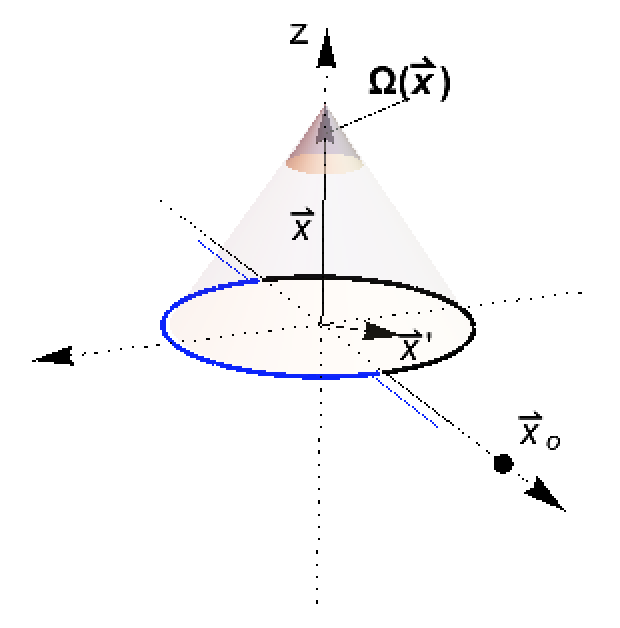
\includegraphics[width=7cm, height=7cm]{solid angle.png}
    \caption{\textit{Δύο ημιάπειρες χορδές Dirac. Οι χορδές τρέχουν παράλληλα κατά μήκος ενός άξονα, σε απειροστά μικρή απόσταση μεταξύ τους, και στη συνέχεια κατά μήκος αντιδιαμετρικών ημικυκλίων ακτίνας $R '$ και κέντρο την αρχή των αξόνων. Κάθε χορδή τερματίζεται στο σημείο $\vec{x}_0$. %αλληλοεπικαλύπτονται σχεδόν παντού και είναι παράλληλες με %ένα κύριο άξονα. Η τοποθέτησή τους περιέχει ημικυκλικό %τομέα με ακτίνα $R '$ ως προς την αρχή των αξόνων. Οι δύο %τομείς είναι στο ίδιο επίπεδο (x-y) αλλά δεν %αλληλοεπικαλύπτονται. Η χορδή τερματίζει στο σημείο 
    }}
    \label{fig:solidangle}
\end{figure}

Εκτελούμε το πρώτο επιφανειακό ολοκλήρωμα της \eqref{vecpotdif3} πραγατοποιώντας το πρώτο. Η επιφάνεια $S$ είναι ο δίσκος
\begin{equation*}
    \pvec{x}' = \big\{ \, (x',\y',0)\quad|\quad \sqrt{x'^2+\y'^2}\le R \, \big\} \quad \forall \, \pvec{x}'\in S
\end{equation*}
Σε πολικές συντεταγμένες έχουμε $\pvec{x}' = \rho'\hat{\rho}'$, %το διαφορικό στοιχείο επιφάνειας 
$d\pvec{s}' = \rho' d\rho' d\phi' \hat{z}$ και το σημείο παρατήρησης είναι το $\vec{x} = \rho\hat{\rho}+z\hat{z}$. Για χάριν απλότητας επιλέγουμε το σημείο παρατήρησης στον άξονα $z$ ($\rho = 0$) και παίρνουμε
\begin{equation}\label{apx_solidangle1}
    \scafun{\Omega}{\vec{x}} \,=\, \int\limits_0^{R}\int\limits_0^{2\pi} \frac{\rho'\hat{\rho}'-z\hat{z}}{\left(z^2+\rho'^2\right)^{3/2}}\cdot \rho'd\rho'd\phi'\hat{z} \,=\, -\int\limits_0^{R}\int\limits_0^{2\pi}\frac{z\,\rho'd\rho'd\phi'}{\left(z^2+\rho'^2\right)^{3/2}}
\end{equation}
\\

Με προσεκτική διερεύνηση, μπορούμε να διακρίνουμε την πλειοτιμία της \eqref{apx_solidangle1}. Στο όριο που προσεγγίζουμε την επιφάνεια από τον θετικό άξονα z ($z\rightarrow 0^+$), παίρνουμε\footnote{Για τη δεύτερη ισότητα έγινε η αντικατάσταση $\rho'\rightarrow\frac{\rho'}{|z|}$.}
\begin{equation}\label{apx_solidangle2}
    \scafun{\Omega}{\vec{x}}\,=\,-\lim\limits_{z\rightarrow 0^+}2\pi\int\limits_0^{R}\frac{z\,\rho'd\rho'}{\left(z^2+\rho'^2\right)^{3/2}} \,=\, -\lim\limits_{z\rightarrow 0^+}2\pi\int\limits_0^{R/z}\frac{\rho'd\rho'}{\left(1+\rho'^2\right)^{3/2}} \,=\, -2\pi
\end{equation}
Στο όριο που προσεγγίζουμε την επιφάνεια από τον αρνητικό άξονα των $z$ ($z\rightarrow 0^-$), παίρνουμε\footnote{Επειδή το $z$ είναι αρνητικό, ο αριθμητής είναι θετικός.} 
%πρέπει να χειριστούμε με σύνεση το αρνητικό πρόσιμο που φέρει %το z στον αριθμητή. Η \eqref{apx_solidangle1} μας δίνει τώρα
\begin{equation}\label{apx_solidangle3}
    \scafun{\Omega}{\vec{x}}\,=\, \lim\limits_{z\rightarrow 0^-}2\pi\int\limits_0^{R/z}\frac{\rho'd\rho'}{\left(1+\rho'^2\right)^{3/2}} \,=\, +2\pi
\end{equation}

Τα αποτελέσματα \eqref{apx_solidangle2} και \eqref{apx_solidangle3} είναι ανεξάρτητα της ακτίνας και του επιπέδου στο οποίο βρίσκεται ο δίσκος. 
%του συνόρου και του προσανατολισμού της επίπεδης επιφάνειας %S\footnote{Η αποδοχή του πιο πάνω είναι εύκολη διαισθητικά %αφού, ως προς ένα σημείο μάνω σε κάποια επίπεδη επιφάνεια, η %γωνία που πρέπει να καλύψουμε ακολουθώντας  ολόκληρο το κλειστό %σύνορο της επιφάνειας είναι $2\pi$ . Από που πλησιάζουμε το %σημείο αυτό της επιφάνειας καθορίζει και το πρόσιμο της στερεάς %γωνίας}. 
Συνοψίζοντας, έχουμε τα ακόλουθα
\begin{equation*}
    \scafun{\Omega}{\vec{x}} \,\rightarrow\, \left\{\begin{array}{cc} -2\pi & z \rightarrow 0^+\\ 2\pi & z\rightarrow0^-
            \end{array} \right. 
\end{equation*}
Διαμέσου της επιφάνειας $S$ του σχήματος \ref{fig:solidangle} ($\vec{x}\rightarrow\pvec{x}'\in S$) η συνάρτηση $\scafun{\Omega}{\vec{x}}$ αλλάζει πρόσημο. Έτσι, η κλίση της είναι 
\begin{equation}\label{derivsolidangle}
    \lim\limits_{\vec{x}\rightarrow\pvec{x}'\in S} \vec{\nabla} \Omega(\vec{x}) = -4\pi \, \scafun{\delta}{z}\hat{z}
\end{equation}
\\
O δεύτερος όρος της \eqref{vecpotdif3} υπολογίζεται ως εξής
\begin{equation}\label{apx_deltaint}
    \int\limits_S  \scafun{\delta}{\vec{x}-\pvec{x}'} d\pvec{s}' \,=\, \int\limits_0^R\int\limits_0^{2\pi}\scafun{\delta}{z\hat{z}-\rho'\hat{\rho}'}\rho'd\rho'd\phi'\hat{z} = \int\limits_0^R\int\limits_0^{2\pi}\frac{\scafun{\delta}{z}\scafun{\delta}{\rho'}}{2\pi\rho'}\rho'd\rho'd\phi'\hat{z} = \scafun{\delta}{z}\hat{z}
\end{equation}
Αντικαθιστώντας τις \eqref{derivsolidangle} και \eqref{apx_deltaint} στην \eqref{vecpotdif3}, συμπεραίνουμε ότι η διαφορά \eqref{vecpotdif3} είναι καλά ορισμένη. 


\subsection{Μεταβολή δράσης Eistein-Hilbert}\label{EHvar}

\begin{equation}
    \delta\R[\rho]{\mu}[\lambda]{\nu} \,=\, \partial\subscr{\lambda}\delta\Gamma\superscr{\rho}\subscr{\;\;\mu\nu} \,+\, \delta\Gamma\superscr{\rho}\subscr{\;\;\lambda\sigma}\Gamma\superscr{\sigma}\subscr{\;\;\mu\nu} \,+\, \Gamma\superscr{\rho}\subscr{\;\;\lambda\sigma}\delta\Gamma\superscr{\sigma}\subscr{\;\;\mu\nu} \,-\, \partial\subscr{\nu}\delta\Gamma\superscr{\rho}\subscr{\;\;\mu\lambda} \,-\, \delta\Gamma\superscr{\rho}\subscr{\;\;\nu\sigma}\Gamma\superscr{\sigma}\subscr{\;\;\mu\lambda} \,-\, \Gamma\superscr{\rho}\subscr{\;\;\nu\sigma}\delta\Gamma\superscr{\sigma}\subscr{\;\;\mu\lambda}
\end{equation}
\begin{equation}
    \nabla\subscr{\lambda}\left(\delta\con{\rho}{\mu}{\nu}\right) \,=\, \partial\subscr{\lambda}\delta\Gamma\superscr{\rho}\subscr{\;\;\mu\nu} \,+\, \Gamma\superscr{\rho}\subscr{\;\;\sigma\lambda}\delta\Gamma\superscr{\sigma}\subscr{\;\;\mu\nu} \,-\, \Gamma\superscr{\sigma}\subscr{\;\;\nu\lambda}\delta\Gamma\superscr{\rho}\subscr{\;\;\mu\sigma} \,-\, \con{\sigma}{\mu}{\lambda}\delta\con{\rho}{\nu}{\sigma}
\end{equation}
\begin{equation}
    \nabla\subscr{\nu}\left(\delta\con{\rho}{\mu}{\lambda}\right) \,=\, \partial\subscr{\nu}\delta\con{\rho}{\mu}{\lambda} \,+\, \con{\rho}{\sigma}{\nu}\delta\con{\sigma}{\mu}{\lambda} \,-\, \con{\sigma}{\lambda}{\nu}\delta\con{\rho}{\mu}{\sigma} \,-\, \con{\sigma}{\mu}{\nu}\delta\con{\rho}{\sigma}{\lambda}
\end{equation}
\begin{equation}
    \delta\R[\rho]{\mu}[\lambda]{\nu} \,=\, \nabla\subscr{\lambda}\delta\con{\rho}{\mu}{\nu} \,-\, \nabla\subscr{\nu}\delta\con{\rho}{\mu}{\lambda}
\end{equation}
\begin{equation}
    \delta\R{\mu}{\nu} \,=\, \delta\R[\lambda]{\mu}[\lambda]{\nu} \,=\, \nabla\subscr{\lambda}\delta\con{\lambda}{\mu}{\nu} \,-\, \nabla\subscr{\nu}\delta\con{\lambda}{\mu}{\lambda}
\end{equation}
\begin{equation}
\begin{split}
    \int \sqrt{-g} \,\g[i]{\mu}{\nu}\,\delta\R{\mu}{\nu}\,d\superscr{4}x \,&=\, \int \sqrt{-g} \,\g[i]{\mu}{\nu} \,\left( \nabla\subscr{\lambda}\delta\con{\lambda}{\mu}{\nu} \,-\, \nabla\subscr{\nu}\delta\con{\lambda}{\mu}{\lambda} \right)\,d\superscr{4}x\\
    &=\, \int\,\sqrt{-g}\left( \nabla\subscr{\lambda}\left(\g[i]{\mu}{\nu}\delta\con{\lambda}{\mu}{\nu}\right) \,-\, \nabla\subscr{\nu}\left(\g[i]{\mu}{\nu}\delta\con{\lambda}{\mu}{\lambda}\right) \right)\,d\superscr{4}x\\
    &=\, \int\,\sqrt{-g}\,\nabla\subscr{\nu}\left(\g[i]{\mu}{\lambda}\delta\con{\nu}{\mu}{\lambda} \,-\,\g[i]{\mu}{\nu}\delta\con{\lambda}{\mu}{\lambda} \right)\,d\superscr{4}x\\
    &=\, 0
    \end{split}
\end{equation}

\subsection{Μεταβολή δράσης Maxwell}\label{Maxwvar}
%Τα σύμβολα ολοκλήρωσης $\int d\superscr{4}x$ αγνοήθηκαν λόγω $συνωστισμού
\begin{equation}
\begin{split}
    \de\subscr{g} L\subscr{M}&=-\frac{1}{4}F\subscr{\mu\nu}F\subscr{\alpha\beta}\left( \de\g[1]{\mu}{\alpha}\g[1]{\nu}{\beta} \,+\, \g[1]{\mu}{\alpha}\de\g[1]{\nu}{\beta} \right)\sqrt{-g}\,\,-\,\,\frac{1}{4}F\superscr{2}\de\sqrt{-g}\\
    &=-\frac{1}{4}\left(F\subscr{\mu\nu}F\subscr{\alpha\beta} \de\g[1]{\mu}{\alpha}\g[1]{\nu}{\beta} \,+\, F\subscr{\nu\mu}F\subscr{\beta\alpha}\g[1]{\nu}{\beta}\de\g[1]{\mu}{\alpha} \right)\sqrt{-g}\,\,-\,\,\frac{1}{4}F\superscr{2}(-\frac{1}{2}\sqrt{-g}\g{\mu}{\alpha}\de\g[1]{\mu}{\alpha})\\
    &=-\left(\frac{1}{2}F\subscr{\mu\nu}F\subscr{\alpha\beta} \de\g[1]{\mu}{\alpha}\g[1]{\nu}{\beta}\,\,-\,\,\frac{1}{8}F\superscr{2}\g{\mu}{alpha}\right)\sqrt{-g}\de\g[1]{\mu}{\alpha}
\end{split}
\end{equation}

\section{Λύση διαφορικής εξίσωσης \ref{differential equation for metric components}}\label{solution for metric dif eq}
Η διαφορική εξίσωση πρώτου βαθμού είναι γραμμική και μη ομογενής. Γράφεται στην ακόλουθη μορφή για τον προσδιορισμό του ολοκληρωτικού παράγοντα 
%(πολλαπλασιαστής Euler) 
$\mu(r)$
\begin{equation}
\begin{split}
    &2r\frac{db}{dr}+e^{2b}(1-\frac{A}{r\superscr{2}})-1=0\\
    &2\frac{db}{dr}e\superscr{-2b}+(\frac{1}{r}-\frac{A}{r\superscr{3}})-\frac{e\superscr{-2b}}{r}=0\\
    &\frac{d}{dr}(e\superscr{-2b})+\frac{e\superscr{-2b}}{r}=\left(\frac{1}{r}-\frac{A}{r\superscr{3}} \right)\\
\end{split}
\end{equation}
Με την αντικατάσταση $\y\equiv e\superscr{-2b}$ 
\begin{equation}\label{inappendix reference differential equation}
    \y'+\frac{1}{r}\y - \left(\frac{1}{r}-\frac{A}{r\superscr{3}} \right) = 0
\end{equation}
η εξίσωση παίρνει τη μορφή 
\begin{equation}
    N(r,\y)\y' + M(r,\y)=0
\end{equation}
επιτρέποντας τον προσδιορισμό του $\mu(r)$
\begin{equation}
    \mu(r) = \exp\left( \int \frac{M\subscr{\y}-N\subscr{r}}{N} \right) = \exp\left( \int \frac{1}{r} dr \right) = r
\end{equation}
Πολλαπλασιάζοντας τώρα την \eqref{inappendix reference differential equation} με $\mu$, η δ.ε. γίνεται
\begin{equation}
    \frac{d}{dr}(\mu y) = \mu \left( \frac{1}{r}-\frac{A}{r\superscr{3}} \right)
\end{equation}
η λύση της οποίας είναι επίσης λύση της \eqref{inappendix reference differential equation}. Oλοκληρώνοντας στο διάστημα $[r\subscr{o},r]$ ($r\subscr{o}\ne0$), βρίσκουμε τη γενική λύση 
\begin{equation}
    \y(r) = 1+\frac{A}{r\superscr{2}}-\frac{c(r\subscr{o})}{r}\quad\Rightarrow\quad b(r)=-\frac{1}{2}\ln\left(1+\frac{A}{r\superscr{2}}-\frac{c(r\subscr{o})}{r}\right)
\end{equation}
\newpage
\chapter{Τανυστικές εξισώσεις στη Mathematica}\label{mathematica}

\begin{mathematica}[Ορισμός Διανύσματος θέσης, μετρικής, αντιστρόφου]\label{mathematica_position_n_metric}
\begin{lstlisting}[language=mathematica]
    x = {t, r, θ, φ};
    g = {{-Exp[2a[r]],0,0,0}, 
            {0,Exp[2b[r]],0,0}, 
                {0,0,r^2,0},
                    {0,0,0,r^2*Sin[ θ ]^2}};
    ginv = Simplify[Inverse[g]];
\end{lstlisting}
\end{mathematica}

\begin{mathematica}[Σύμβολα Christoffel]\label{mathematica_chr_symbols}
\begin{lstlisting}[language=mathematica]
    CS = Simplify[Table[1/2 (
       Sum[
        ginv[[i,z]]*D[g[[j,z]],x[[k]]],{z,4}] 
      +Sum[
        ginv[[i,z]]*D[g[[k,z]],x[[j]]],{z,4}]
      -Sum[
        ginv[[i,z]]*D[g[[j,k]],x[[z]]],{z,4}]),
        {i,4}, {j,4}, {k,4}
    ]];
\end{lstlisting}
\end{mathematica}

\begin{mathematica}[Τανυστής Riemann]\label{mathematica_Riemann}
\begin{lstlisting}[language=mathematica]
    Riemmann = Simplify[Table[
        D[ CS[[i, j, z]], x[[k]]] 
      +Sum[ CS[[i,k,s]]
        * CS[[s,j,z]], {s,4}] 
      -Sum[ CS[[i,z,s]]
        * CS[[s,j,k]], {s,4}],
      {i,4}, {j,4}, {k,4}, {z,4}
    ]];
\end{lstlisting}
\end{mathematica}

\begin{mathematica}[Τανυστής Ricci]\label{mathematica_Ricci}
\begin{lstlisting}[language=mathematica]
    Ricci = Simplify[Table[
        Sum[
         Riemmann[[i,j,i,z]], {i,4}], 
        {j,4}, {z,4}
    ]]; 
\end{lstlisting}
\end{mathematica}

\newpage
\begin{mathematica}[Ηλεκτροματνητικός Τανυστής]\label{mathematica_emtensor}
\begin{lstlisting}[language=mathematica]
    F = Table[0,{i,4},{i,4}];
    B[r_] := Q/(2er^2); 
    F[[3,4]] = Q/(2e)*Sin[ θ ];
    F[[4,3]] = -Q/(2e)*Sin[ θ ];
\end{lstlisting}
\end{mathematica}

\begin{mathematica}[Τανυστής ενέργειας-ορμής]\label{mathematica energy momentum tensor}
\begin{lstlisting}[language=mathematica]
    EnergyTensor = Simplify[Table[
    Sum[F[[i, k]]*F[[j,z]]*ginv[[k,z]],{k,4},{z,4}] 
    - 1/4 g[[i,j]]*Sum[
        F[[i,j]]*F[[m,n]]*ginv[[m,i]] ginv[[n,j]], 
        {i,4},{j,4},{m,4},{n,4}], 
    {i,4}, {j,4}]];
\end{lstlisting}
\end{mathematica}

\begin{mathematica}[Ίχνος τανυστή ενέργειας-ορμής]\label{mathematica trace of ene mom ten}
\begin{lstlisting}[language=mathematica]
    Ttrace = Simplify[
        Sum[
            ginv[[i,j]]*EnergyTensor[[i,j]],{i,4},{j,4}]
    ];
\end{lstlisting}
\end{mathematica}

\begin{mathematica}[Δεξιό σκέλος εξίσωσης Einstein]\label{mathematica rs of einstein eq}
\begin{lstlisting}[language=mathematica]
    T = Simplify[Table[
        EnergyTensor[[i,j]] - 1/2Ttrace*g[[i,j]],{i,4},{j,4}]
    ];
\end{lstlisting}
\end{mathematica}

\begin{mathematica}[Εξισώσεις Einstein]\label{mathematica system of einstein equations}
\begin{lstlisting}[language=mathematica]
    For[i = 1, i <= 4, i++, 
        For[j = 1, j <= 4, j++, 
            If[PossibleZeroQ[Ricci[[i, j]]], Null, 
                Print["{", x[[i]], x[[j]], "}", ":", 
                    Simplify[
                        Ricci[[i, j]] - 8*Pi*G*T[[i, j]] == 0
                    ]]]]]
\end{lstlisting}
\end{mathematica}

%---------------------------------------------------------------------------
% Bibliography
%---------------------------------------------------------------------------

%\addcontentsline{toc}{chapter}{\textcolor{tssteelblue}{Literature}}
\begin{english}
\printbibliography[title={\begin{greek}Βιβλιογραφία\end{greek}}]
\end{english}
%---------------------------------------------------------------------------
% Index
%---------------------------------------------------------------------------

%\printindex

\end{document}
